\part{Part 3: Applications}

\graphicspath{ {./Pictures/} }
\chapterimage{chapter_head_2.pdf} % Chapter heading image

%++++++++++++++++++++++++++++++++++++++++++++++++++++++++++++++
\chapter{Introduction}
\label{ch:intro for tutorials}
%++++++++++++++++++++++++++++++++++++++++++++++++++++++++++++++
\section{Gmsh}
\begin{gmshnote}
	Read all about Gmsh and download its source and executables at \href{http://gmsh.info}{http://gmsh.info}.
\end{gmshnote}
Gmsh is an 2D/3D mesh generator including a built-in CAD engine and post-processor. Gmsh was developed to provide a fast, light, and user-friendly meshing environment with additional visualization capabilities. It is open source, and the source code and executables for various operating systems (Windows, Mac, Linux) can be downloaded directly from \href{http://gmsh.info}{http://gmsh.info}. Gmsh contains modules for geometry definition, meshing, solving and post-processing. each module has its own set of commands, which can be easily manipulated using the graphical user-interface (GUI).

Upon launching the Gmsh executable the GUI will open, and the the module panel appears on left-hand side of window with headings to control the:
\begin{itemize}
    \item \textbf{Geometry}
    \item \textbf{Mesh}
    \item \textbf{Solver}
\end{itemize}
The \textbf{Geometry} section is a module that allows you to create your own geometry directly within Gmsh, or import external CAD files. Geometry in Gmsh is defined using a hierarchical structure. This means a volume is made up of different surfaces, and each surface is made up of different curvatures or lines. In turn, each curve or line is bounded by two end points in the case of a straight line, or a sequence of points in the case of a spline, for example. Therefore, to define a desired geometry a set of points are specified first, and the connections between these pints are built by straight lines or curves. Then, a set of surfaces are created using the lines and curves, which are themselves used to define a volume in the case of a three-dimensional problem.

The geometry module has some key features to allow you to accomplish these tasks. Some of the important features are as follows:
\begin{itemize}
    \item \textbf{Elementary entities}: Create, merge, split or delete points, lines, curves, faces or volumes as needed.
    \item \textbf{Physical groups}: Specify boundary conditions and physical properties (i.e. fluid or solid) of a particular geometric entity.
    \item \textbf{Reload script}: Re-reads the geometry saved in your .geo file, the Gmsh native file format.
    \item \textbf{Edit script}: Allows you to edit the .geo file manually using a text editor.
\end{itemize}
It is worth noting that geometry specifications are saved in the .geo file in plain text format. This allows you to manually manipulate geometry or any other specifications by editing this plain text file using either the in-built text editor, or an external one. 

After building the geometry and defining the boundary conditions via the \textbf{Geometry} module, the next step is usually to generate a discrete mesh of the geometry using the \textbf{Mesh} module. This module splits our geometry up into a number of simple geometric elements, such as: lines, triangles, tetrahedra, hexahedra and pyramids. Gmsh has several different algorithms for automatically generating the mesh, and an unstructured mesh will be generated by default. The \textbf{Mesh} module has also some sections that help to specify the type, number and density of mesh in domain. Here, some of the important sections:
\begin{itemize}
    \item \textbf{Define}: Set the number of grid points and stretching ratios. Additionally, control the mesh type (whether structured or unstructured).
    \item \textbf{2D/3D}: Generates the mesh for surfaces/volumes in domain. It automatically generates the mesh using specifications provided in the \textbf{Define} section.
    \item 
\end{itemize}
Additionally, there is another module named \textbf{Solver}, which allows a numerical solver to be accessed directly from Gmsh. In the context of the current book, this will not be used here.

\section{SU2}
\begin{su2note}
	Read all about SU2 and download its source and executables at \href{https://su2code.github.io/}{https://su2code.github.io/}.
\end{su2note}
As discussed in the Physics and Numerics parts of this book, ultimately an approximate solution to the Navier-Stokes or RANS equations is obtained by solving a discrete system of equations on a computational grid, or mesh. SU2 is an open-source CFD solver built specifically for this task. SU2 is written in C++, and its primary applications are computational aerodynamics and shape optimization. SU2 is generally user-friendly, and pre-compiled versions are available for all major operating systems (Windows, Mac, Linux). In the following laboratories we will demonstrate the utility of SU2 as a CFD tool for computational aerodynamics. Additional details on the capabilities of SU2, its source code, executables, and several example applications are available at \href{https://su2code.github.io/}{https://su2code.github.io/}.

%++++++++++++++++++++++++++++++++++++++++++++++++++++++++++++++
\section{Paraview}
\begin{paraviewnote}
	Read all about Paraview and download its source and executables at \href{https://www.paraview.org/}{https://www.paraview.org/}.
\end{paraviewnote}
After SU2 runs it generates a set of data files, which includes the complete flow field solved on the mesh generated previously using Gmsh. This data must be post-processed to visualize the flow structures, such as the velocity or pressure distributions. Paraview is an open-source and multi-platform visualization tool designed for this task. It is also available for all operating systems (Windows, Mac, Linux) and is free to download and use. Paraview is designed specifically to handle large complex data sets, such as those generated in CFD simulations. In the following laboratory experiments, we will use Paraview as a post-processing tool for the analysis of the data produced by SU2. Typically, this analysis consists of contours of flow parameters, extracting line plots, slices, or pressure coefficient distributions. Additional details about Paraview, its source code, executables, and example datasets can be found at \href{https://www.paraview.org/}{https://www.paraview.org/}.

%++++++++++++++++++++++++++++++++++++++++++++++++++++++++++++++
\chapter{Inviscid NACA0012}
\label{ch:Inviscid NACA0012}
%++++++++++++++++++++++++++++++++++++++++++++++++++++++++++++++
\section{Required Files}
\begin{su2note}
	Use the following links to download the same version of SU2 for Windows (\href{}{click here}) or Mac (\href{}{click here}), and the required configuration (\href{}{click here}) and mesh files (\href{}{click here}).
\end{su2note}
\begin{paraviewnote}
	Use the following links to download the same version of Paraview for Windows (\href{}{click here}) or Mac (\href{}{click here}).
\end{paraviewnote}

\section{Problem Description}
In this tutorial we are going to demonstrate how to simulate inviscid flow around the well-known NACA0012 airfoil. Under the assumption of inviscid flow, the Euler equations will be used. Please note that this assumption is only reasonably valid at high Reynolds numbers and low angles of attack, since the contribution of the viscous terms in the Navier-Stokes equations is minimal in this case. The flow specifications are provided as follows:
\begin{itemize}
    \item Pressure = 101,325 Pa
    \item Temperature = 273 K
    \item Mach number = 0.8
    \item Angle of attack = 1.25 degree
\end{itemize}
This tutorial has two parts: Flow Solution and Post-Processing. In the first part we will explain how to manage the required files and settings in SU2, and then run the simulation. In the second part we will explore how to use Paraview to visualize data files generated in the first step by SU2.
%++++++++++++++++++++++++++++++++++++++++++++++++++++++++++++++
\section{Flow solution}
To run this simulation SU2 needs two files: a configuration file (.cfg) and a mesh file (.su2). Links to the required files and executables are provided at the start of this tutorial. The files include:
\begin{enumerate}
\item \textit{inv\_NACA0012}.cfg: the configuration file.
\item \textit{mesh\_NACA0012\_inv}.su2: the mesh file.
\end{enumerate}
The next step is to copy these two files in the directory you have save the SU2 executable, so everything is located in the same folder. Then, to run the simulation using the executable, mesh, and configuration files simply open a terminal window and enter the following commands:
\begin{table}[htbp]
    \centering
    \begin{tabular}{|l|l|}
    \hline
    Windows     & \begin{tabular}{c} \$ cd "where you saved the package" \\ \$ SU2\_CFD.exe inv\_NACA0012.cfg \end{tabular}
    \\
    \hline
    Mac     & \begin{tabular}{c} \$ cd "where you saved the package" \\ \$ SU2\_CFD.exe inv\_NACA0012.cfg \end{tabular}
    \\
    \hline
    \end{tabular}
\end{table}

The SU2 solver will commence solving the problem and will print out the residuals at every iteration, until the specified convergence criteria is achieved. After the calculations are complete the following output files should have been generated within in the SU2 folder:
\begin{itemize}
    \item \textit{flow}.vtk: The flow solution on the entire domain.
    \item \textit{force\_breakdown}.dat: Forces and moment on the airfoil.
    \item \textit{history}.vtk: Convergence history.
    \item \textit{restart\_flow}.dat: Restart file.
    \item \textit{surface\_flow}.vtk: The flow solution on the airfoil surface.
    \item \textit{surface\_flow}.csv: A comma separated value file of the flow solution on the airfoil.
\end{itemize}
Please keep in mind that every time you run SU2, the output data will be overwritten. Hence, before launching a new simulation you should backup your files in another directory.
%++++++++++++++++++++++++++++++++++++++++++++++++++++++++++++++
\section{Post-Processing}
In this section, we explain how to use Paraview to visualize the solution generated by SU2. First of all, install paraview using the links at the start of this tutorial. Once that is complete, perform the following steps to visualize the results:
%--------------------------------------------------------------
\subsection{Open the Solution:}
Launch Paraview. Go to \textbf{File} $\rightarrow$ \textbf{Open}, and then select \textit{flow}.vtk file. On the left-hand side of the Paraview window you will see the file appears under \textbf{builtin} in the \textbf{Pipeline Browser}. Now press the \textbf{Apply} button in the \textbf{Properties} tab, right under the \textbf{Pipeline Browser} heading. After taking these steps, your file is loaded by Paraview and is ready to be visualized (Figure \ref{fig1:load}).
\begin{figure}[htbp]
    \centering
    \includegraphics[width=0.4\textwidth]{tut01/loadvtkfile.pdf}
    \caption{Loading .vtk file in the \textbf{Pipeline Browser}.}
    \label{fig1:load}
\end{figure}
%--------------------------------------------------------------
\subsection{Visualize the Mesh}
In order to view the mesh that was stored in the .su2 file, and as shown in Figure \ref{fig1:wireframe}, select \textit{Solid Color} with \textit{Wireframe} in the toolbar. Then, you can zoom in to see the mesh near the surface of the airfoil. as shown in Figure \ref{fig1:mesh}. As you can see, the mesh around the NACA0012 is unstructured, and the elements are clustered around the leading and trailing edges of the to resolve the complex flow structures that are expected there.
\begin{figure}[htbp]
    \centering
    \includegraphics[width=0.6\textwidth]{tut01/wireframe.pdf}
    \caption{How to display mesh in computational domain.}
    \label{fig1:wireframe}
\end{figure}
\begin{figure}[htbp]
    \centering
    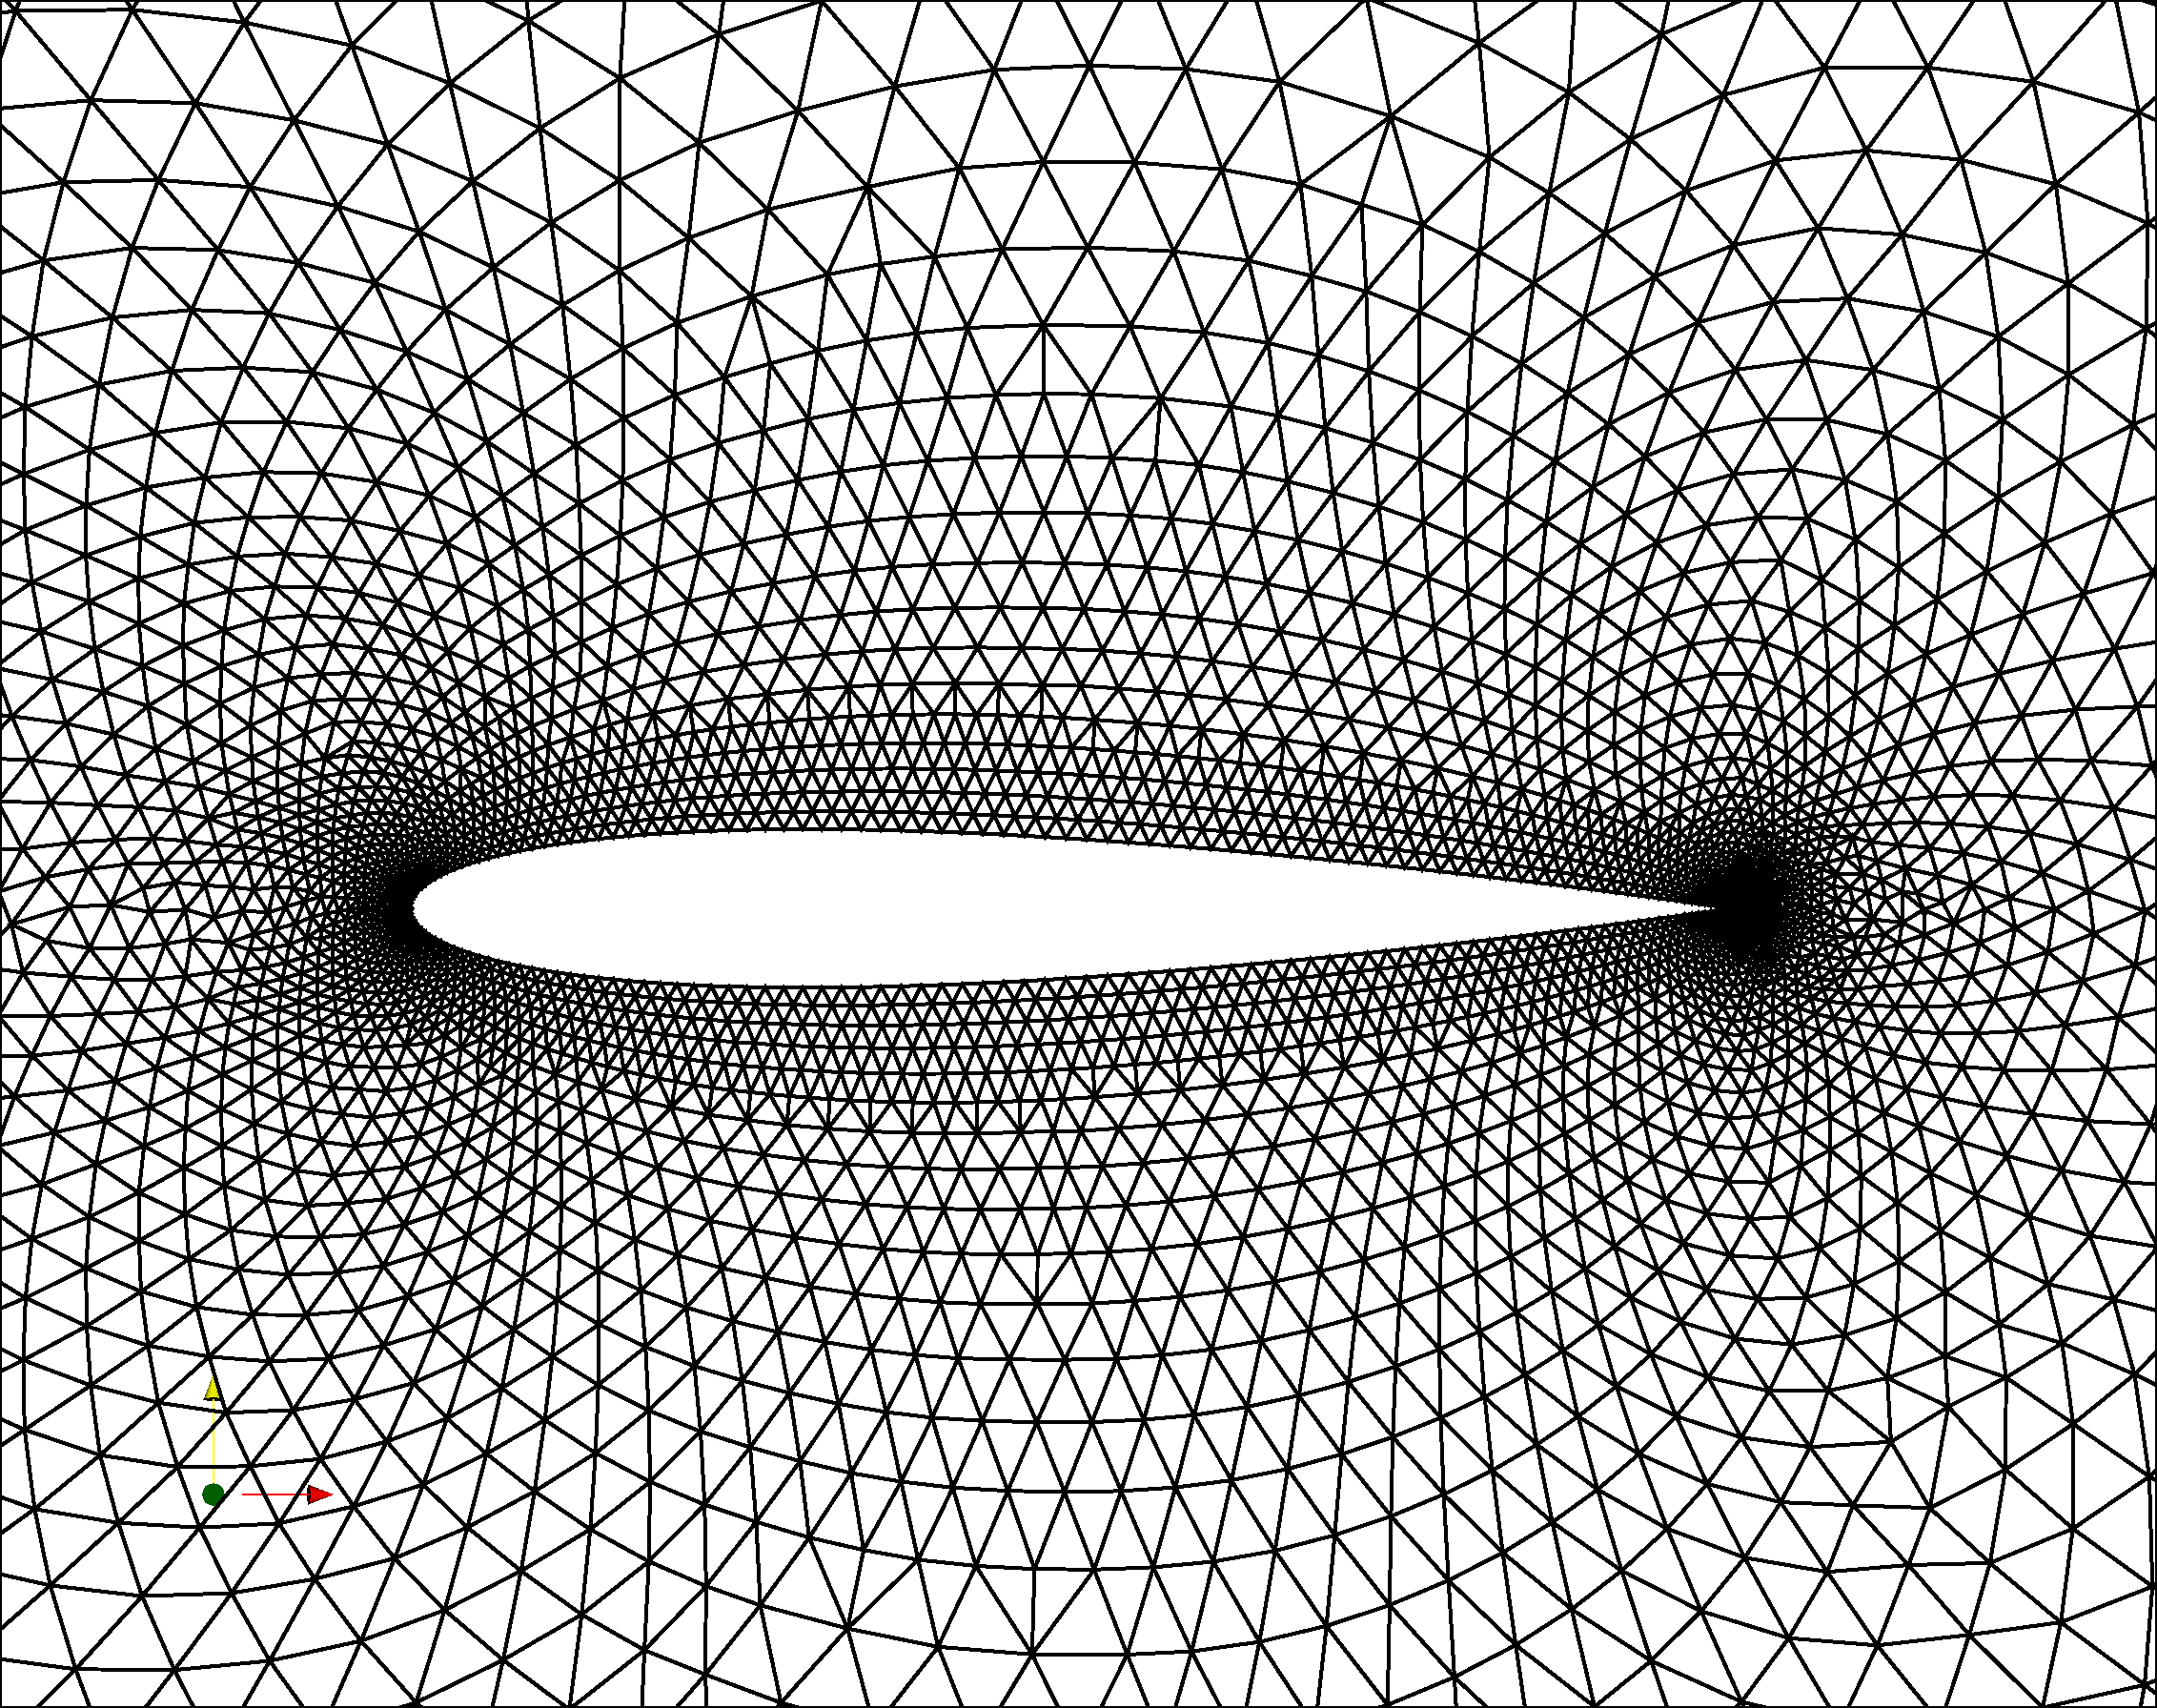
\includegraphics[width=.75\textwidth]{tut01/mesh.pdf}
    \caption{Unstructured mesh around NACA0012.}
    \label{fig1:mesh}
\end{figure}
%--------------------------------------------------------------
\subsection{Visualize Pressure Contour}
In order to visualize pressure contours, click on \textit{flow}.vtk from within the \textbf{Pipeline Browser} to select the current data file, and then click on the \textbf{Properties} tab. According to Figure \ref{fig1:colorby}, in \textbf{Coloring} section, select \textit{Pressure} from the drop-down menu. To change the color settings used to show the pressure field you can click on \textbf{Edit} under the \textbf{Coloring} options. Another display window appears on the right-hand side of the monitor, similar to Figure \ref{fig1:change_color_range}. Now you can change the maximum/minimum range of pressure to your desired values using the \textbf{Set Range} option, or change the contour colors using \textbf{Choose Preset} (Figure \ref{fig1:change_color_range}).
\begin{figure}[htbp]
    \centering
    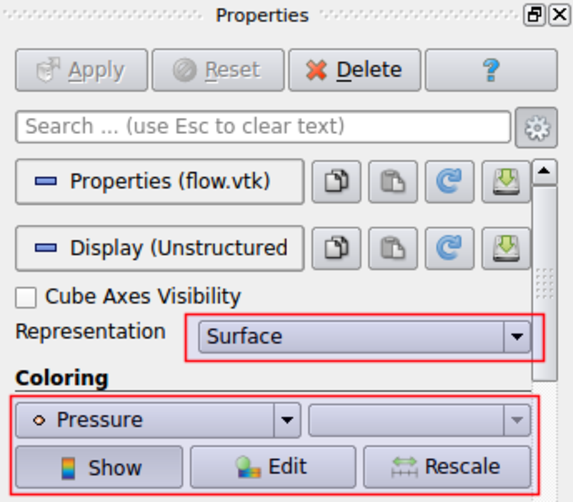
\includegraphics[width=0.4\textwidth]{tut01/contourdisplay.pdf}
    \caption{Contour settings in \textbf{Display} tab.}
    \label{fig1:colorby}
\end{figure}
\begin{figure}[htbp]
    \centering
    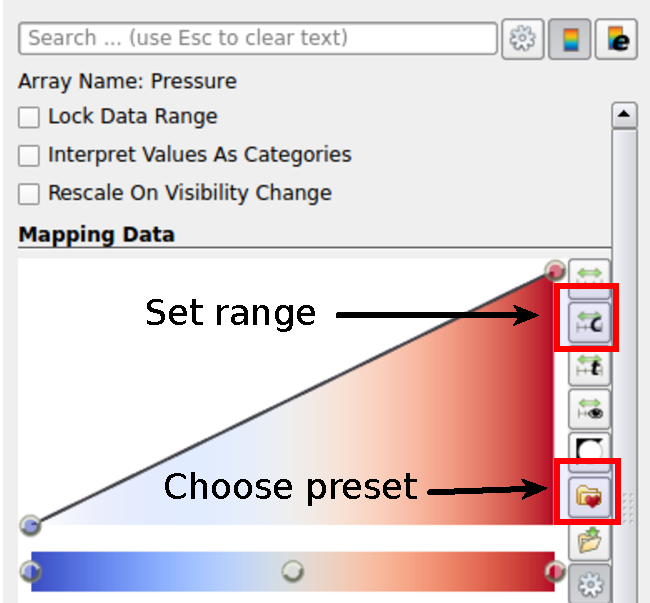
\includegraphics[width=0.5\textwidth]{tut01/colormap.pdf}
    \caption{How to change color and max/min values for contour.}
    \label{fig1:change_color_range}
\end{figure}
After these steps, the pressure contours shown in the display window should be similar to those shown in Figure \ref{fig1:pressure_contour}.
\begin{figure}[htbp]
    \centering
    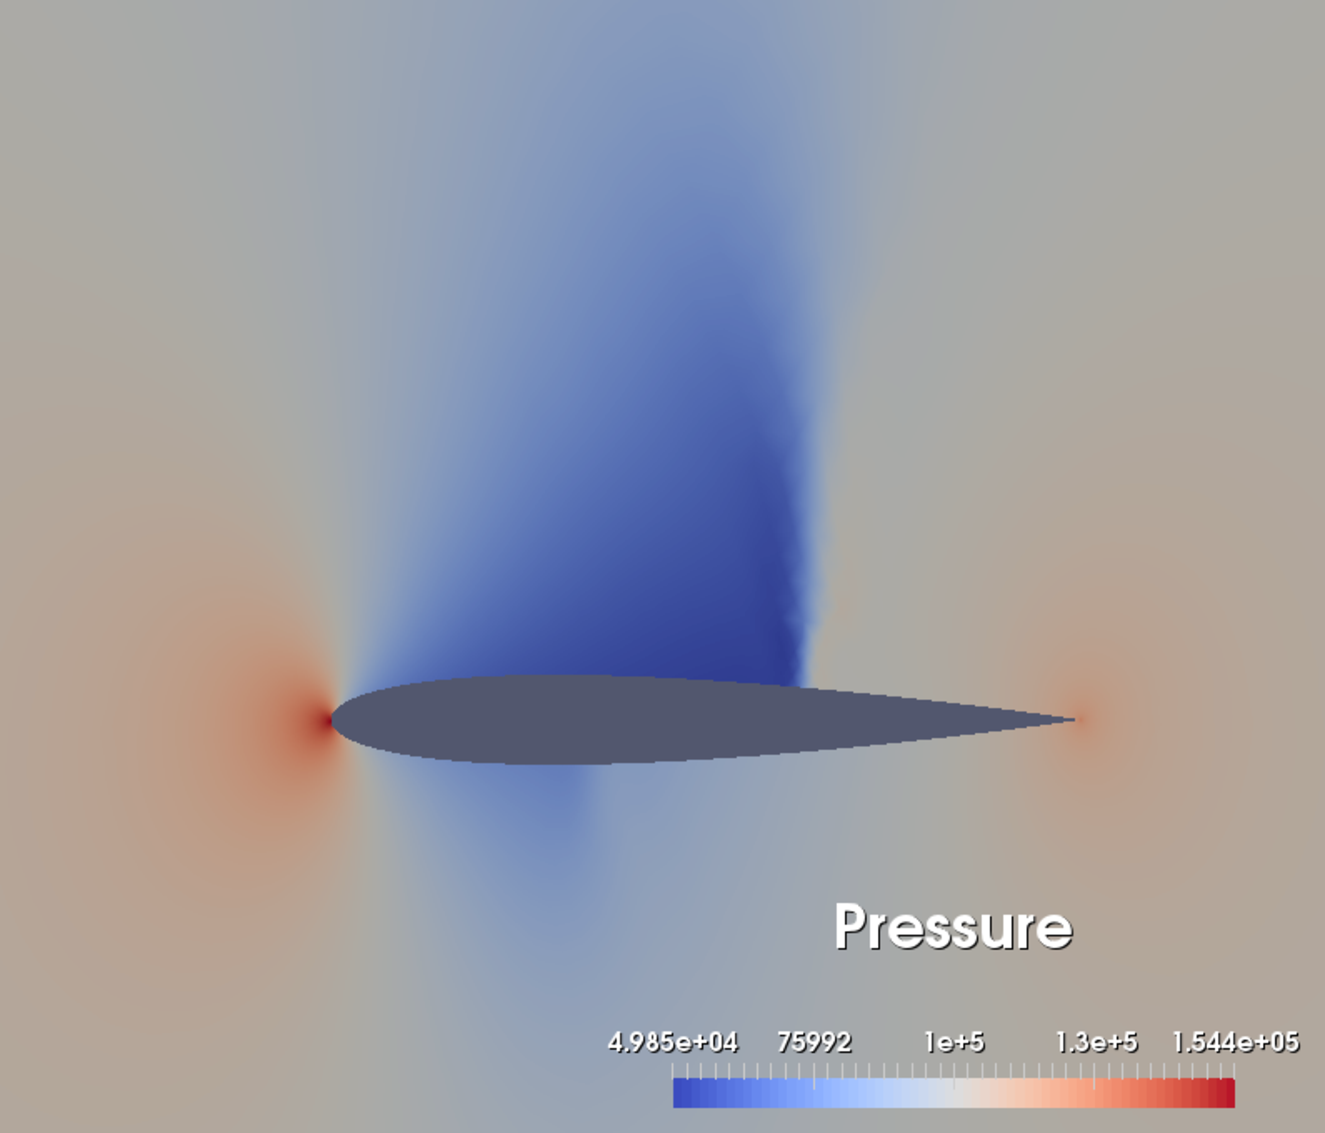
\includegraphics[width=.75\textwidth]{tut01/pressurecontour1.pdf}
    \caption{Pressure contour for NACA0012 airfoil.}
    \label{fig1:pressure_contour}
\end{figure}

To add contour lines, click again on the \textit{flow}.vtk file in the \textbf{Pipeline Browser}, and then click on the \textbf{Contour} icon (Figure \ref{fig1:contour_icon}) in the toolbar.
\begin{figure}[htbp]
    \centering
    \includegraphics[width=0.6\textwidth]{tut01/contourlineicon.pdf}
    \caption{Contour icon in the toolbar.}
    \label{fig1:contour_icon}
\end{figure}
Now you should see that a new item called \textit{Contour1} appears under \textit{flow}.vtk in the \textbf{Pipeline Browser} (Figure \ref{fig1:contour1}).
\begin{figure}[htbp]
    \centering
    \includegraphics[width=0.5\textwidth]{tut01/contour1.pdf}
    \caption{Adding \textit{Contour1} in \textbf{Pipeline Browser}.}
    \label{fig1:contour1}
\end{figure}
As shown in Figure \ref{fig1:contourby a}, go to the \textbf{Properties} tab, and select \textit{Pressure} from the \textbf{Contour By} drop-down menu. Next, click on the \textbf{New Range} icon to customize the range of contour lines that will be generated. For now, set the number of steps to 20, similar to Figure \ref{fig1:contourby b}. This means the pressure contour range is equally divided by 20 portions between the minimum and maximum values. Finally, click on \textbf{Apply} to generate these contour lines in the display window.
\begin{figure}[htbp]
    \centering
     \begin{subfigure}[b]{.4\textwidth}
         \centering
         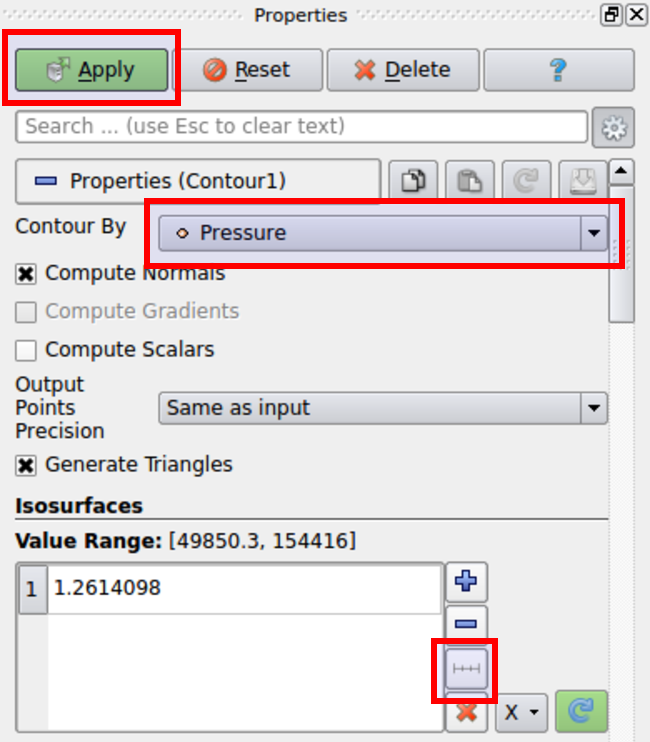
\includegraphics[width=1.0\textwidth]{tut01/contourlinenewrange.pdf}
         \caption{Define new range}
         \label{fig1:contourby a}
     \end{subfigure}
     \hfill
     \begin{subfigure}[b]{.4\textwidth}
         \centering
         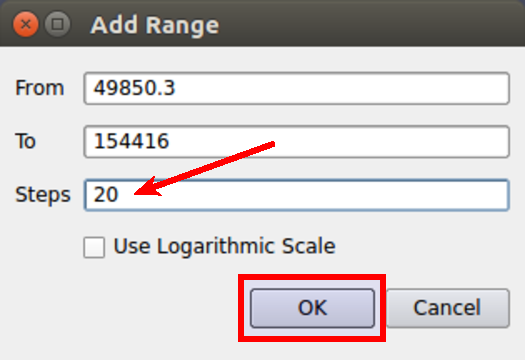
\includegraphics[width=1.0\textwidth]{tut01/addrangepdf.pdf}
         \caption{Add range}
         \label{fig1:contourby b}
     \end{subfigure}     
    \caption{How to define a new range for the contour lines.}
    \label{fig1:contourby}
\end{figure}
Next, as it is shown in Figure \ref{fig1:colorby2}, click on the \textbf{Display} under \textbf{Properties} tab. In the \textbf{Coloring} section, select \textbf{Solid Color} from the drop-down menu, and choose white as the color using \textbf{Edit}.
\begin{figure}[htbp]
    \centering
    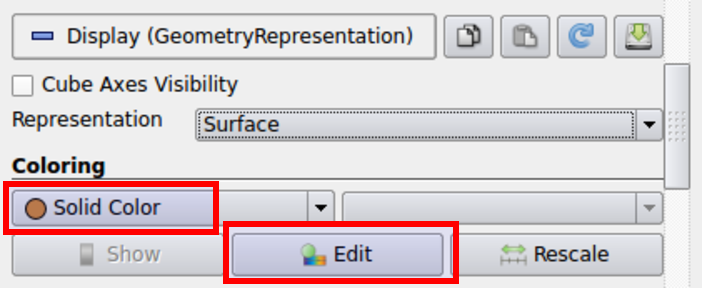
\includegraphics[width=0.6\textwidth]{tut01/coloring.pdf}
    \caption{Changing contour lines color in \textbf{Coloring} section.}
    \label{fig1:colorby2}
\end{figure}
Now the pressure contour lines should look similar to Figure \ref{fig1:pressure_contour_lines}.
\begin{figure}[htbp]
    \centering
    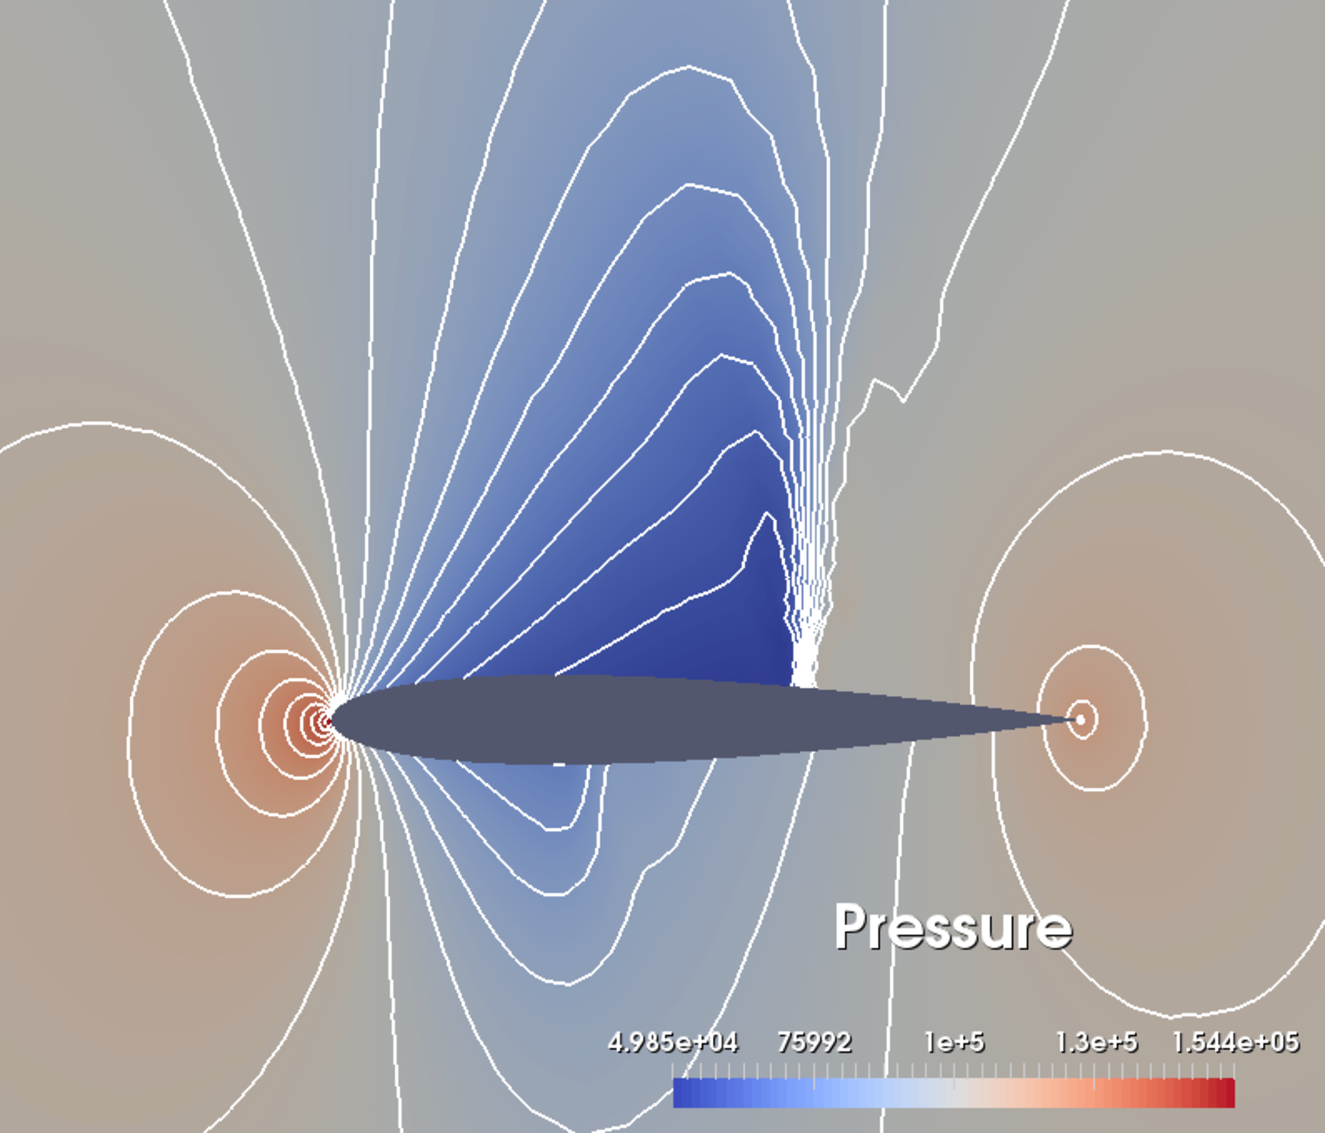
\includegraphics[width=.75\textwidth]{tut01/pressurecontour2.pdf}
    \caption{Pressure contour superimposed by contour lines around NACA0012.}
    \label{fig1:pressure_contour_lines}
\end{figure}
%--------------------------------------------------------------
\subsection{Visualize Pressure Coefficient}
The pressure data on the surface of the airfoil is stored in \textit{surface\_flow}.vtk. We will now generate a plot of the pressure coefficient as a function of chordwise position. Go to \textbf{Open} $\rightarrow$ \textbf{File} and select \textit{surface\_flow}.vtk. As shown in Figure \ref{fig1:builtin}, this file is now loaded and added to the list of items under \textbf{builtin} in \textbf{Pipeline Browser}.
\begin{figure}[htbp]
    \centering
    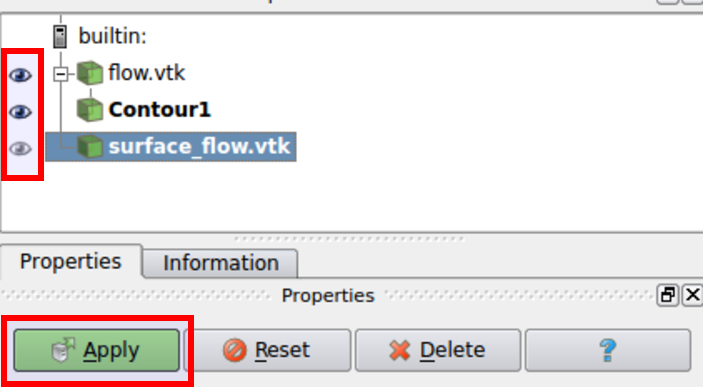
\includegraphics[width=0.5\textwidth]{tut01/eyeiconsurfaceflow.pdf}
    \caption{Loading another .vtk file in Paraview.}
    \label{fig1:builtin}
\end{figure}
Note that there is an eye icon on the left-hand side of each item in \textbf{Pipeline Browser}, which enables you to hide/unhide the plots related to each item. Since we want to see only the pressure coefficient plot, we hide the previously-generated contours by unselecting the eye icon beside \textit{flow}.vtk and \textit{Contour1}. 

As shown in Figure \ref{fig1:plotdata}, select \textit{surface\_flow}.vtk in \textbf{Pipeline Browser} and then go to \textbf{Filters} $\rightarrow$ \textbf{Search} (Figure \ref{fig1:plotdata a}) and search for \textbf{Plot Data} (Figure \ref{fig1:plotdata b}). 
\begin{figure}[htbp]
    \centering
     \begin{subfigure}[b]{.4\textwidth}
         \centering
         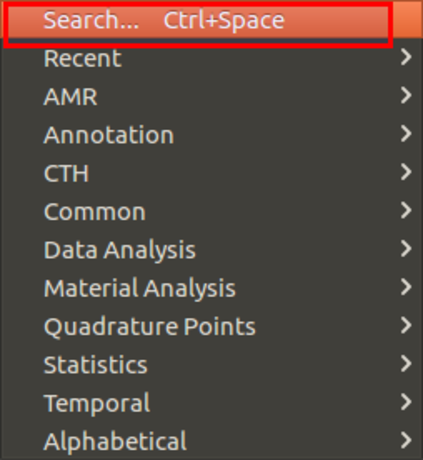
\includegraphics[width=1.0\textwidth]{tut01/filtersearch.pdf}
         \caption{Search item in \textbf{Filter}}
         \label{fig1:plotdata a}
     \end{subfigure}
     \hfill
     \begin{subfigure}[b]{.4\textwidth}
         \centering
         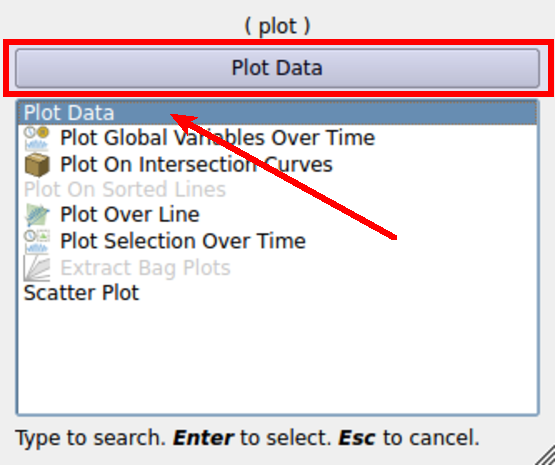
\includegraphics[width=1.0\textwidth]{tut01/plotdatasearch.pdf}
         \caption{Searching for \textbf{PotData}}
         \label{fig1:plotdata b}
     \end{subfigure}     
    \caption{How to plot data.}
    \label{fig1:plotdata}
\end{figure}

After taking this step, as shown in Figure \ref{fig1:plotdata-list}, the \textit{PlotData1} item is added to tthe \textbf{Pipeline Browser}. Hide (deactivate) all items in the list of \textbf{Pipeline Browser} except \textit{PlotData1} by clicking on the eye icons beside each item, and then click on \textbf{Apply}.
\begin{figure}[htbp]
    \centering
    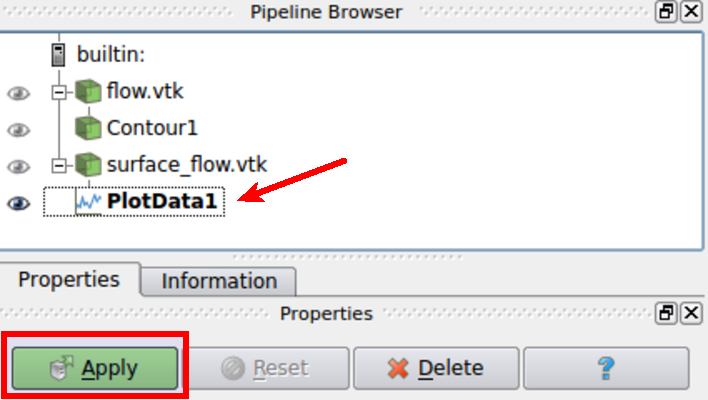
\includegraphics[width=0.5\textwidth]{tut01/plotdata1.pdf}
    \caption{Adding \textit{PlotData1} to \textbf{Pipeline Browser}.}
    \label{fig1:plotdata-list}
\end{figure}
As shown in Figure \ref{fig1:pointsx}, from \textbf{Display} in the \textbf{Properties} tab, deactivate \textbf{Use Index For XAxis}, and then select \textit{Points\_X} from the drop-down menu. 
\begin{figure}[htbp]
    \centering
    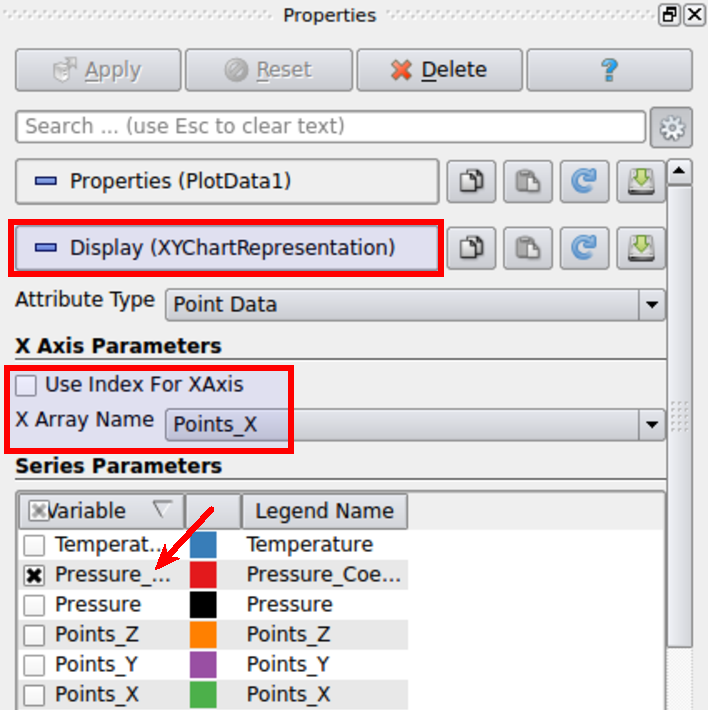
\includegraphics[width=0.5\textwidth]{tut01/plotcurvesetting.pdf}
    \caption{Plot settings for pressure coefficient along the chord line.}
    \label{fig1:pointsx}
\end{figure}
In the \textbf{Series Parameters} in the same tab, unselect all variables except for \textit{Pressure\_Coefficient}. This allows you to have only one plot showing the pressure coefficient versus chord line. The pressure plot in the display window should be similar to Figure \ref{fig1:surface_pressure}.
\begin{figure}[htbp]
    \centering
    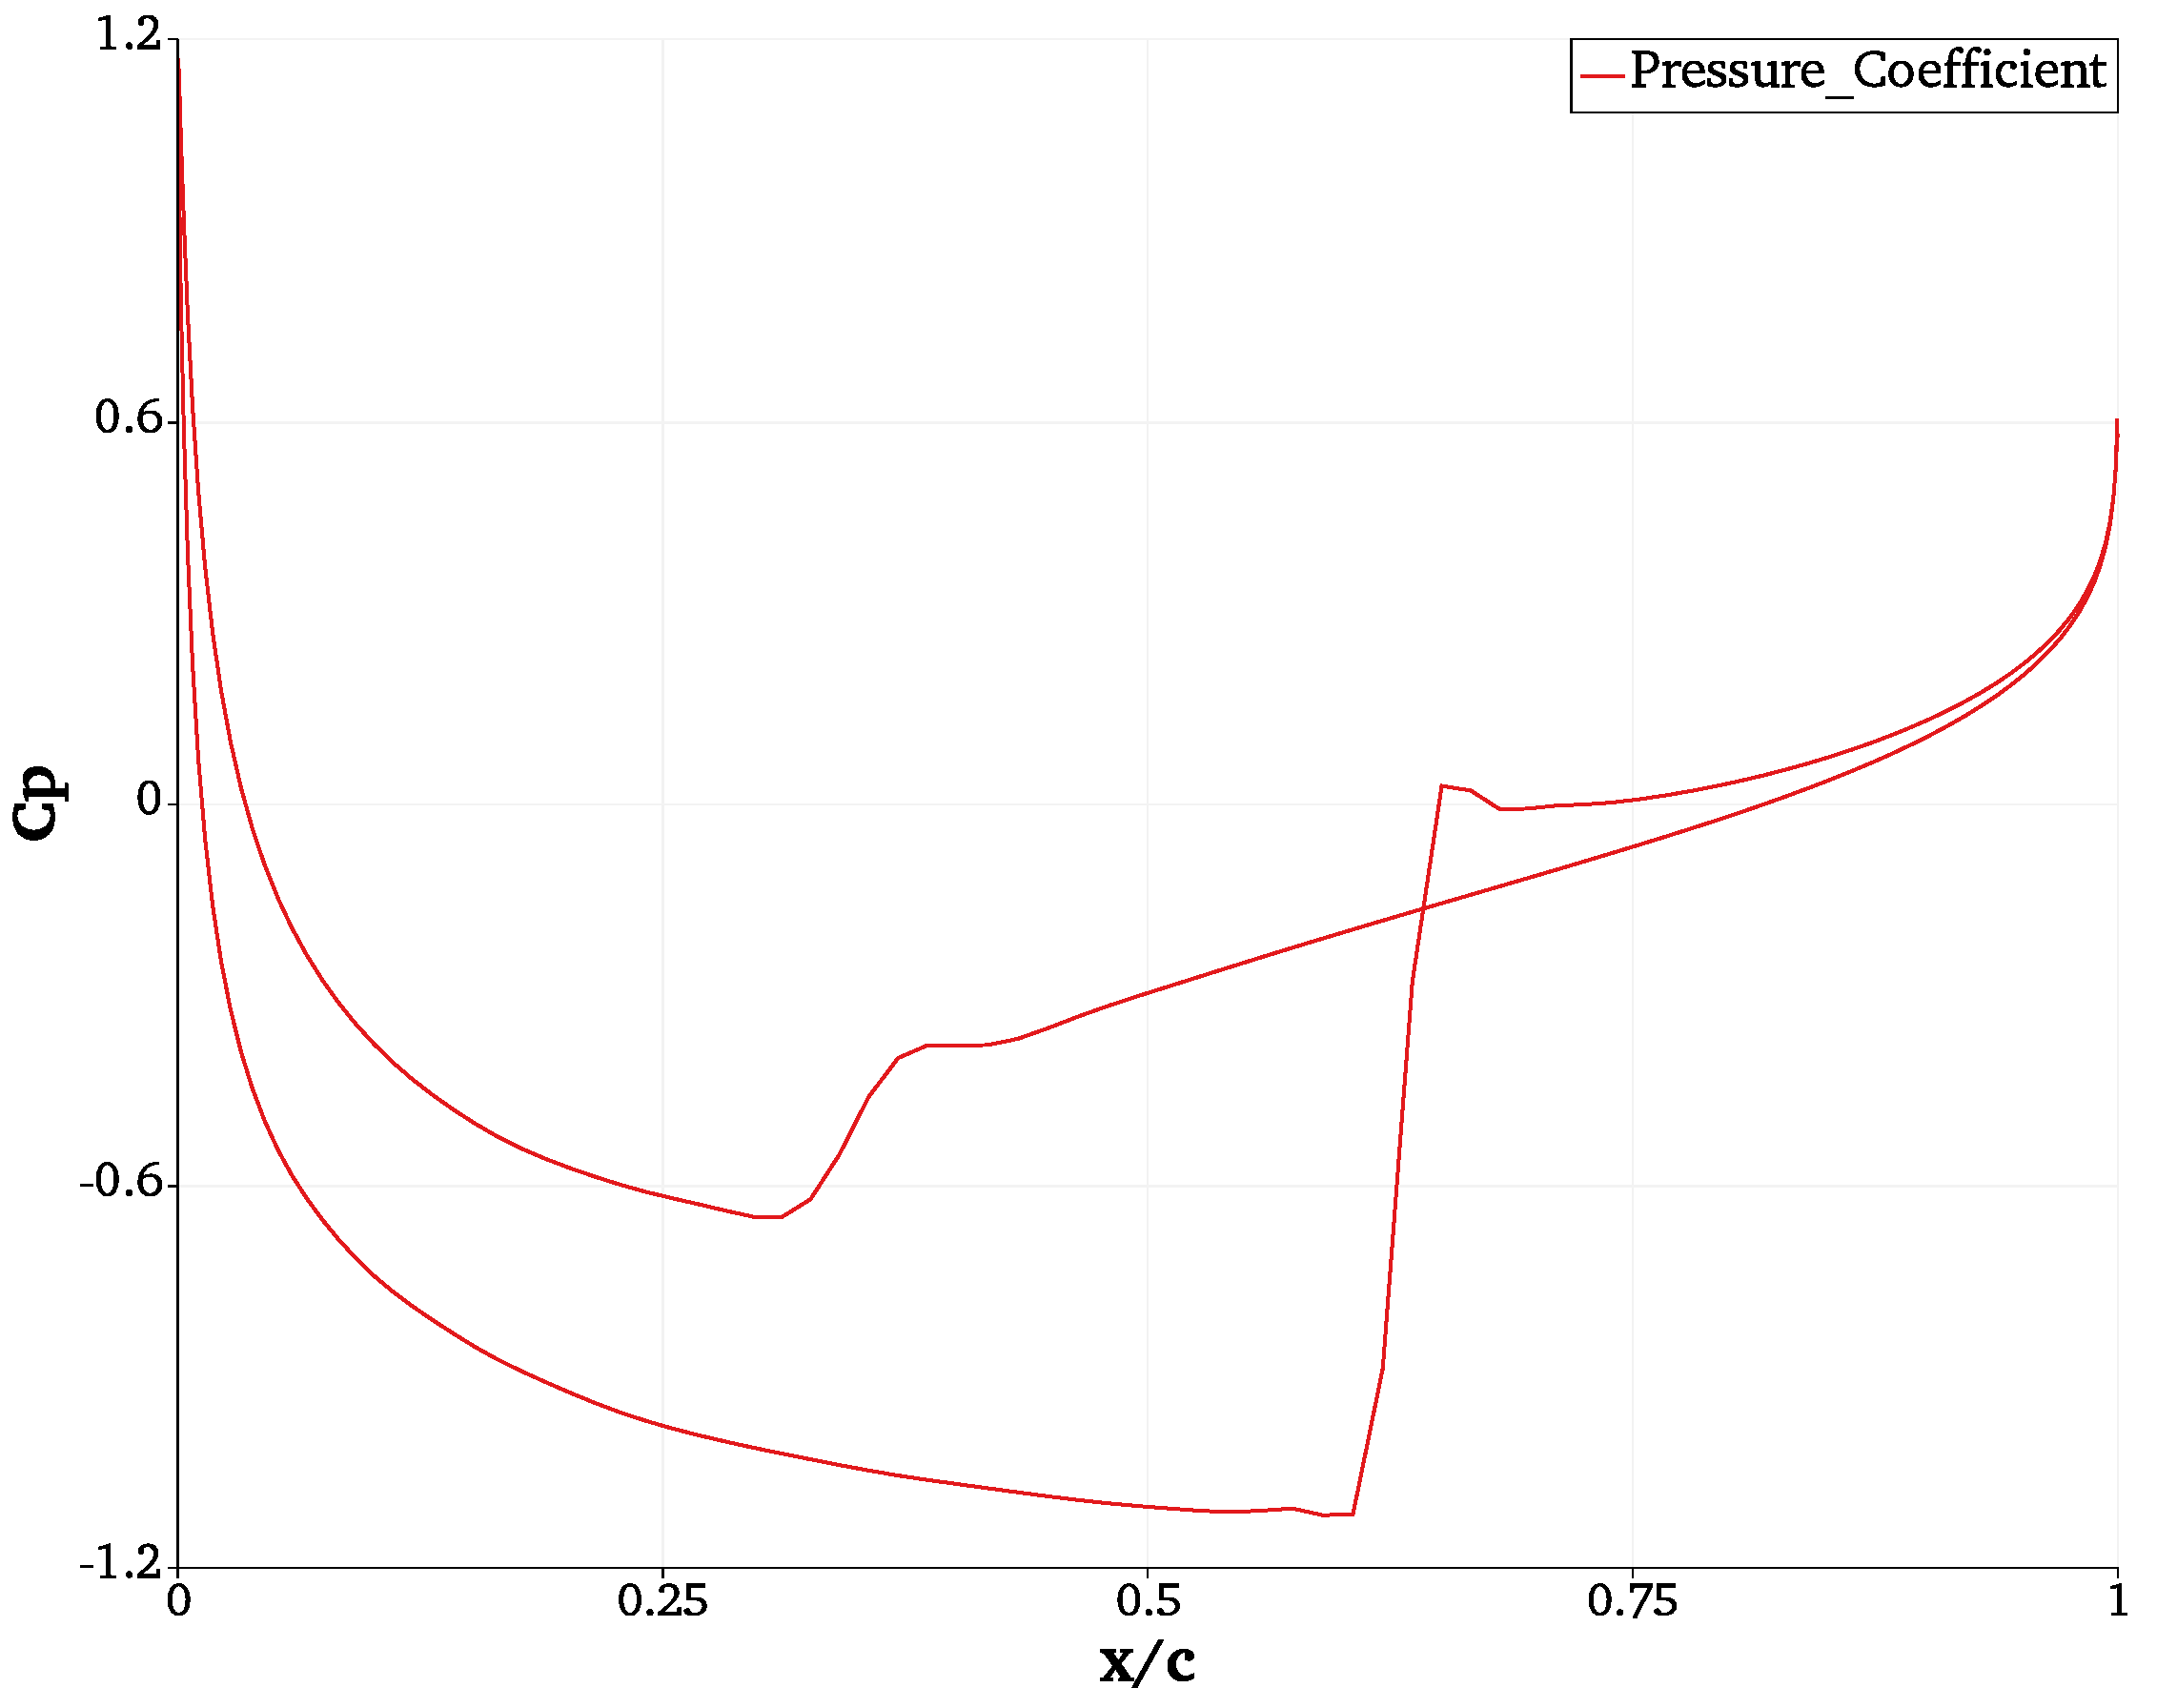
\includegraphics[width=.75\textwidth]{tut01/plot11.pdf}
    \caption{Pressure coefficient on the surface of the NACA0012.}
    \label{fig1:surface_pressure}
\end{figure}

By convection, $-C_p$ is typically plotted such that the pressure curve on suction side (lower pressure) is on top of the pressure curve on the pressure side (higher pressure). Therefore, we need to reverse the $y$-axis in this plot to flip it. To do this, go to \textbf{Display} in the \textbf{Properties} tab. Next, find the \textbf{Left Axis Range} section in the same tab, and then click on \textbf{Left Axis Use Custom Range} (Figure \ref{fig1:viewsetting}). Later, another section appears to select maximum/minimum ranges for left axis of plot. Now, switch numbers in these two text bars. This allows the $y$-axis to be reverse (flipped).
\begin{figure}[htbp]
    \centering
    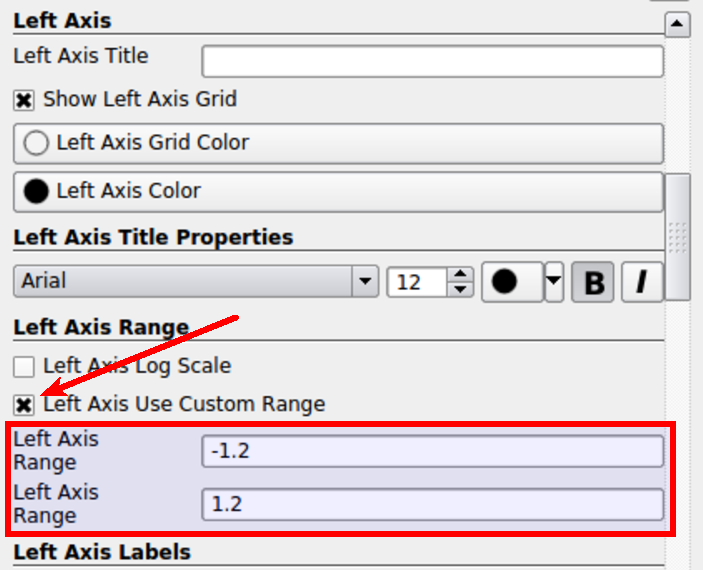
\includegraphics[width=0.5\textwidth]{tut01/leftaxis.pdf}
    \caption{Plot Settings.}
    \label{fig1:viewsetting}
\end{figure}
Additionally, there are other parameters that you may want to change in the same tab, like \textbf{Left Axis Title} or \textbf{Bottom Axis Title}. To do this, please type $C_p$ and $x/c$ in \textbf{Left Axis Title} and \textbf{Bottom Axis Title}, respectively. Furthermore, for adding markers to the plot lines, form \textbf{Display} select the \textbf{Marker Style} as \textit{Diamond} (Figure \ref{fig1:marker}). You can also change the thickness of plot line in the same tab.
\begin{figure}[htbp]
    \centering
    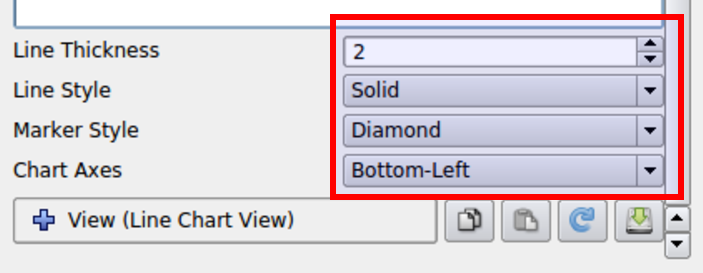
\includegraphics[width=0.4\textwidth]{tut01/addingmarker.pdf}
    \caption{How to add marker to plot.}
    \label{fig1:marker}
\end{figure}
Eventually, the final plot you should get is like Figure \ref{fig1:surface_pressure2}
\begin{figure}[htbp]
    \centering
    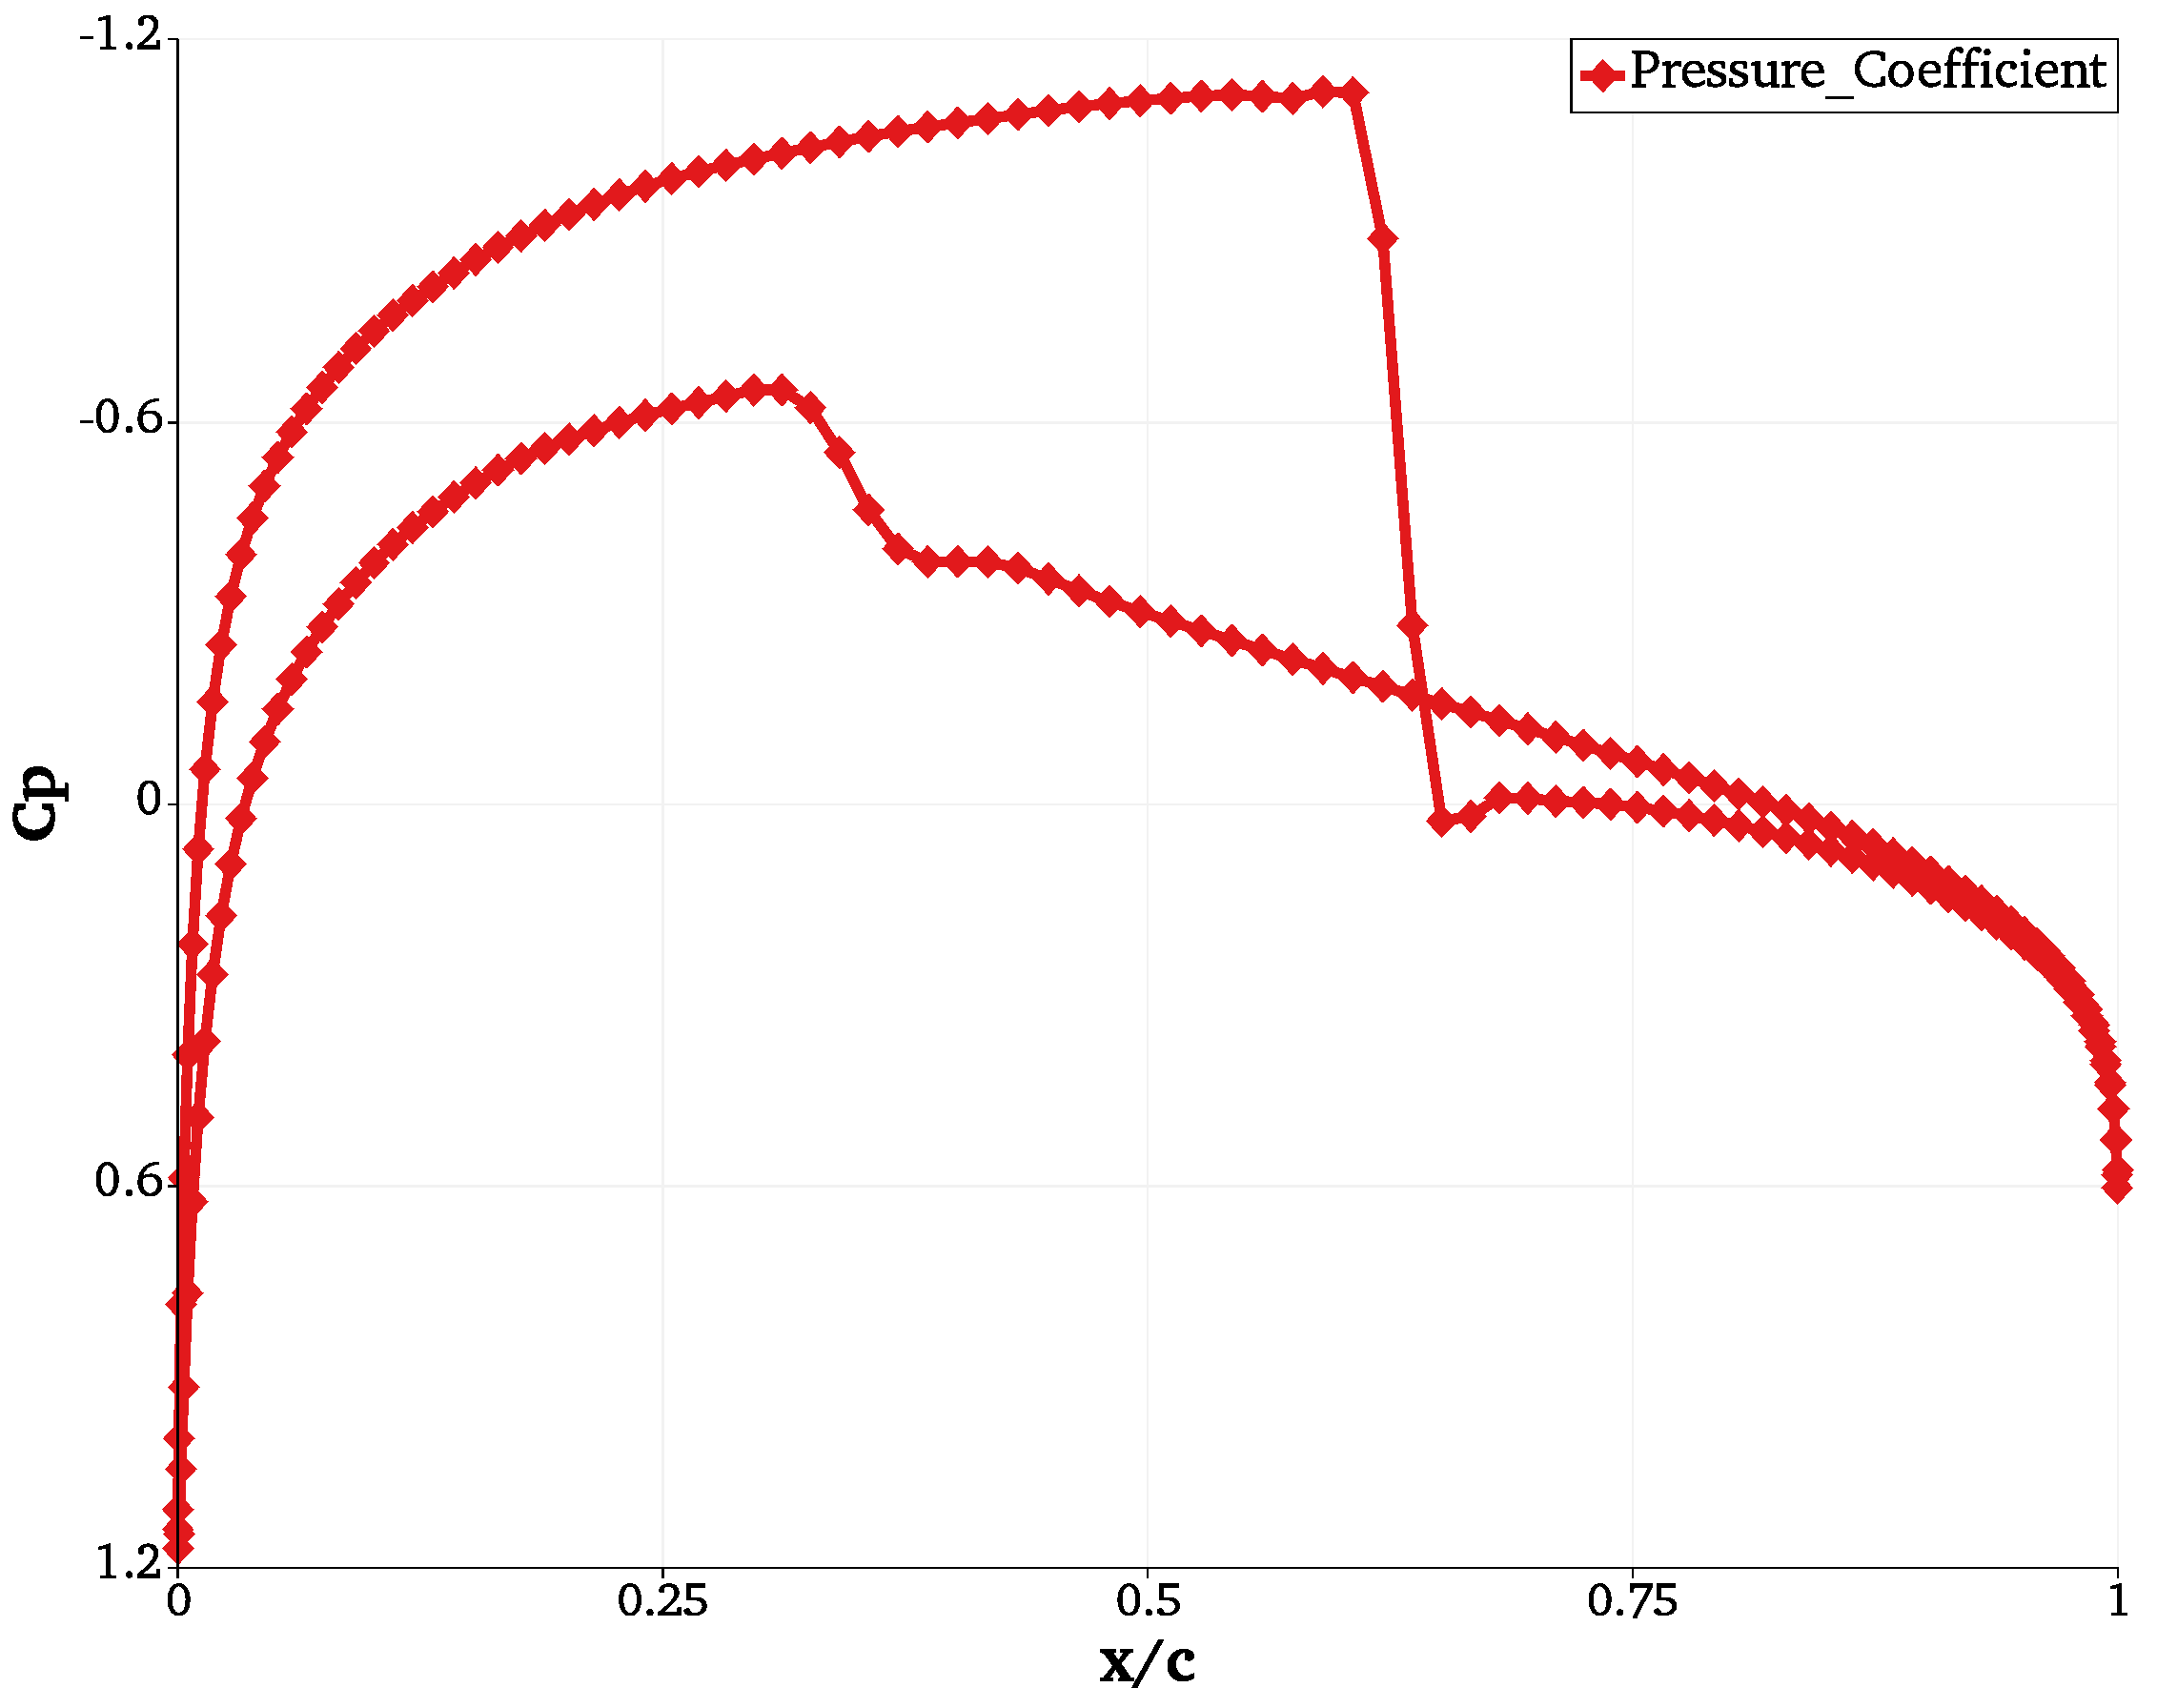
\includegraphics[width=.75\textwidth]{tut01/plot22.pdf}
    \caption{Revised version of the pressure coefficient plot on the surface of the NACA0012.}
    \label{fig1:surface_pressure2}
\end{figure}
%--------------------------------------------------------------
\subsection{Aerodynamic Forces}
In order to obtain the aerodynamic forces on the airfoil, open \textit{force\_breakdown}.dat using a text editor software. According to Figure \ref{fig1:forcefile1}, in this file the flow properties are also show, and it can be confirmed that these agree with the values in the configuration file. 
\begin{figure}[htbp]
    \centering
    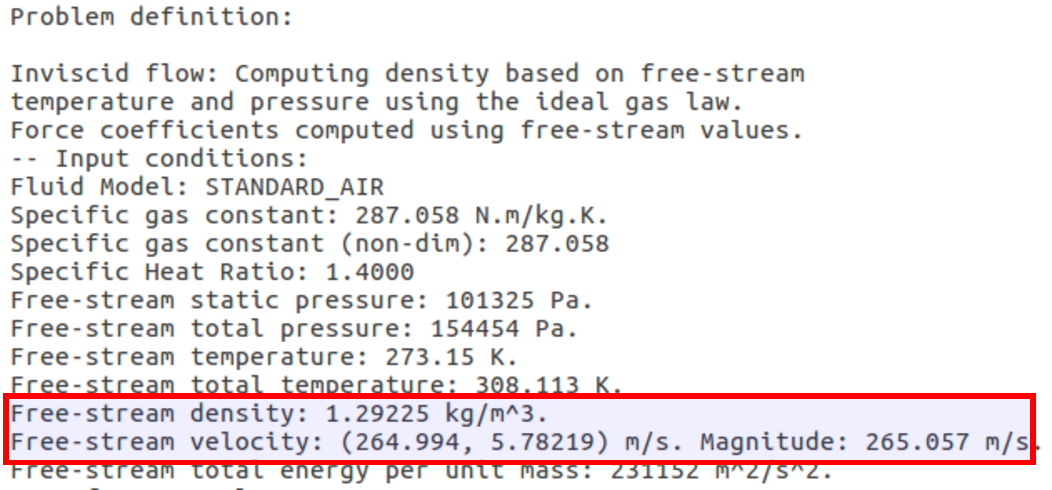
\includegraphics[width=0.9\textwidth]{tut01/forcefile1.pdf}
    \caption{Fluid and flow properties from \textit{force\_breakdown}.dat.}
    \label{fig1:forcefile1}
\end{figure}

Additionally, as shown in Figure \ref{fig1:forcefile2}, the aerodynamic forces are expressed in non-dimensional form by using free-stream values for density and velocity, as well as one reference length (or area). The actual dimensional forces (dimensional) can be obtained by multiplying the flow coefficients with these non-dimensional factor calculated with the free-stream density and velocity. Note that you can find the lift coefficient ($C_L$), drag coefficient ($C_D$), lift to drag ratio ($C_L / C_D$), the moment coefficient ($C_{M,z}$), $x$-component of force coefficient ($C_{F,x}$) and $y$-component of force coefficient ($C_{F,y}$) all from the \textit{force\_breakdown}.dat.
\begin{figure}[htbp]
    \centering
    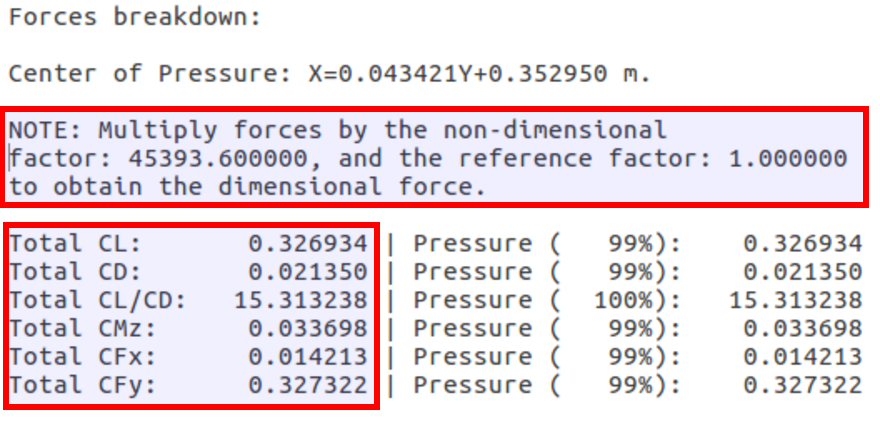
\includegraphics[width=0.8\textwidth]{tut01/forcefile2.pdf}
    \caption{Aerodynamic loads from \textit{force\_breakdown}.dat.}
    \label{fig1:forcefile2}
\end{figure}
%++++++++++++++++++++++++++++++++++++++++++++++++++++++++++++++
\clearpage
\section{Questions}
1. Run the provided default NACA0012 test case at the provided Ma = 0.8.
\begin{enumerate}[label=(\alph*)]
    \item Plot and comment on the mesh.
    \item Plot and comment on the pressure contours around the airfoil.
    \item Plot and comment on the pressure coefficient on the surface of the airfoil.
\end{enumerate}
2. Re-run the default NACA0012 case but change the Mach number to Ma = 0.3 and run several simulations using alpha = 0, 2, 4, 6, 8, 10, 12, 14, 16 degrees.
\begin{enumerate}[label=(\alph*)]
    \item Plots Cl vs alpha alongside the provided experimental data \cite{ladson1988effects} in the test case folder.
    \item Repeat 1.b with Ma = 0.3 for the alpha = 0, 8, 16 degree cases.
    \item Repeat 1.c with for the alpha = 0, 8, 16 degree cases and include the provided experimental data  in the \cite{ladson1987pressure}.
\end{enumerate}
3. Compare your CFD results in Question 2). Discuss sources of error that could have led to any discrepancies in your results.
%--------------------------------------------------------------
%++++++++++++++++++++++++++++++++++++++++++++++++++++++++++++++
%++++++++++++++++++++++++++++++++++++++++++++++++++++++++++++++
%++++++++++++++++++++++++++++++++++++++++++++++++++++++++++++++
\chapter{Supersonic Wedge}
\label{ch:Supersonic Wedge}
%++++++++++++++++++++++++++++++++++++++++++++++++++++++++++++++
\section{Required Files}
\begin{su2note}
	Use the following links to download the same version of SU2 for Windows (\href{}{click here}) or Mac (\href{}{click here}), and the required configuration (\href{}{click here}) and mesh files (\href{}{click here}).
\end{su2note}
\begin{paraviewnote}
	Use the following links to download the same version of Paraview for Windows (\href{}{click here}) or Mac (\href{}{click here}).
\end{paraviewnote}
\section{Problem Description}
In this tutorial we are going to demonstrate how to simulate supersonic inviscid flow past a simple 2D wedge. This wedge generates an oblique-shock wave moving outwards from its surface. Assuming the Reynolds number is high enough, and that the fluid is an ideal gas, we will be using the Euler equations. The domain is approximated using a structured mesh with 3,750 nodes. The domain consists of a flat upper wall, and a lower wall with an inclined a wedge starting at $x/L=1/3$, where $L$ is the length of duct. The wedge angle is taken to be 10 degrees, and the inlet flow paramaters are:
\begin{itemize}
    \item Pressure = 101,325 Pa
    \item Temperature = 273.15 K
    \item Mach number = 2.0
    \item Wedge angle = 10 degrees
\end{itemize}
This tutorial has two parts: Flow Solution and Post-processing. In the first part, we will explain how to manage yjr prerequisite files and settings, and how to run the CFD simulation using SU2. In the second part we explain how to use Paraview to visualize the data obtained from SU2.
%++++++++++++++++++++++++++++++++++++++++++++++++++++++++++++++
\section{Flow solution}
To run this simulation SU2 needs two files: a configuration file (.cfg) and a mesh file (.su2). Links to the required files and executables are provided at the start of this tutorial. The files include:
\begin{enumerate}
    \item inv\_wedge\_HLLC.cfg which is a configuration file.
    \item mesh\_wedge\_inv.su2 which is a a mesh file.
\end{enumerate}
The next step is to copy these two files into that same directory as the SU2 executable. Then, to run the simulation open a terminal window and enter the following commands:
\begin{table}[htbp]
    \centering
    \begin{tabular}{|l|l|}
    \hline
    Windows     & \begin{tabular}{c} \$ cd "where you saved the package" \\ \$ SU2\_CFD.exe inv\_wedge\_HLLC.cfg \end{tabular}
    \\
    \hline
    Mac     & \begin{tabular}{c} \$ cd "where you saved the package" \\ \$ SU2\_CFD.exe inv\_wedge\_HLLC.cfg \end{tabular}
    \\
    \hline
    \end{tabular}
\end{table}

The SU2 solver will commence solving the problem and will print out the residuals at every iteration, until the specified convergence criteria is achieved. After the calculations are complete the following output files should have been generated within in the SU2 folder:
\begin{itemize}
    \item \textit{flow}.vtk: The flow solution on the entire domain.
    \item \textit{force\_breakdown}.dat: Forces and moment on the airfoil.
    \item \textit{history}.vtk: Convergence history.
    \item \textit{restart\_flow}.dat: Restart file.
    \item \textit{surface\_flow}.vtk: The flow solution on the airfoil surface.
    \item \textit{surface\_flow}.csv: A comma separated value file of the flow solution on the airfoil.
\end{itemize}
Please keep in mind that every time you run SU2, the output data will be overwritten. Hence, before launching a new simulation you should backup your files in another directory.
%++++++++++++++++++++++++++++++++++++++++++++++++++++++++++++++
\section{Post-Processing}
In this section, we explain how to use Paraview to visualize the solution generated by SU2. First of all, install paraview (if not already done) using the links at the start of this tutorial. Once that is complete, perform the following steps to visualize the results:
%--------------------------------------------------------------
\subsection{Load Solution File:}
Launch Paraview. Go to \textbf{File} $\rightarrow$ \textbf{Open}, and then select the \textit{flow}.vtk file. On the left side of the Paraview window you will see the file appears in the \textbf{Pipeline Browser} under \textbf{builtin}. Now press the \textbf{Apply} button in the \textbf{Properties} tab, right under the \textbf{Pipeline Browser} heading. After taking these steps, your file is loaded by Paraview and is ready to be visualized (Figure \ref{fig2:load}).
\begin{figure}[htbp]
    \centering
    \includegraphics[width=0.4\textwidth]{tut02/loadvtkfile.pdf}
    \caption{Loading .vtk file in the \textbf{Pipeline Browser}.}
    \label{fig2:load}
\end{figure}
%--------------------------------------------------------------
\subsection{Visualize Mesh Domain}
As shown in Figure \ref{fig2:wireframe}, in order to view the mesh select \textit{Solid Color} with \textit{Wireframe} in the toolbar. Then, you can zoom in to see the mesh for the computational domain, as shown in Figure \ref{fig2:mesh}. As you can see, the mesh in the duct is structured, and at the start of the wedge abruptly changes the direction of mesh on the bottom surface. Additionally, the grids are approximately uniform throughout the domain.
\begin{figure}[htbp]
    \centering
    \includegraphics[width=0.6\textwidth]{tut02/wireframe.pdf}
    \caption{How to display mesh in computational domain.}
    \label{fig2:wireframe}
\end{figure}
\begin{figure}[htbp]
    \centering
    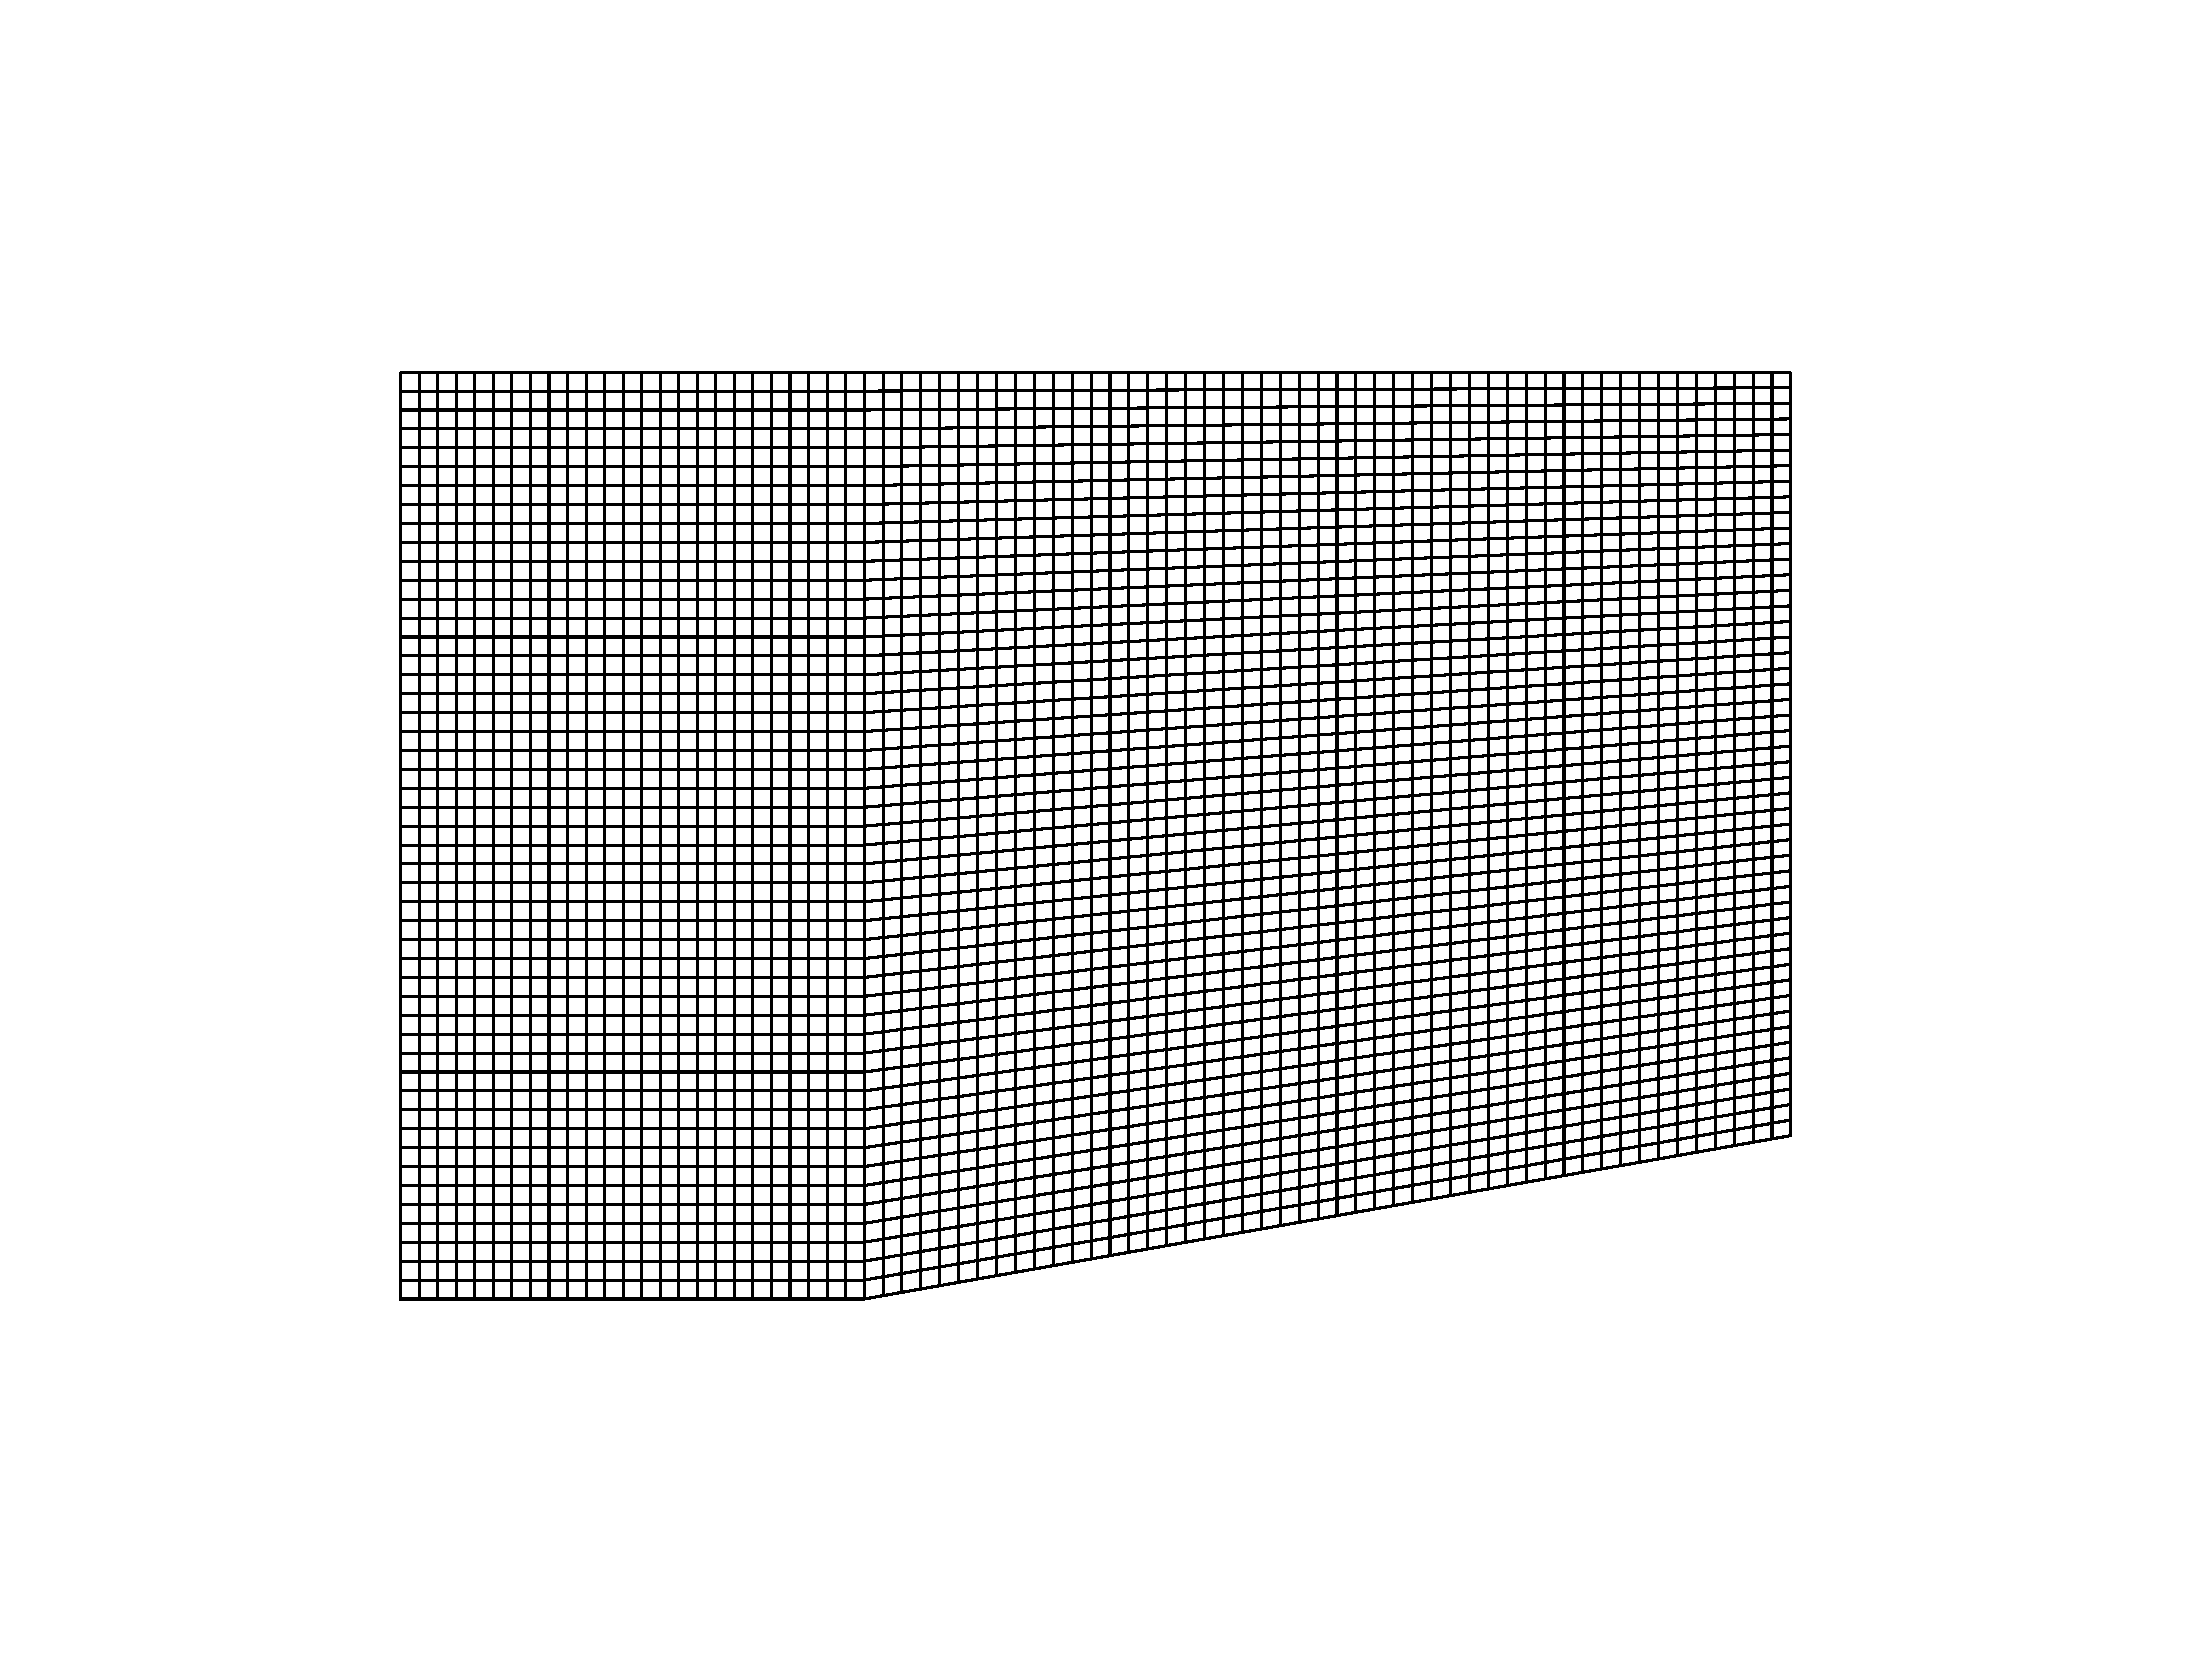
\includegraphics[width=.75\textwidth]{tut02/mesh.pdf}
    \caption{Structured mesh for wedge domain.}
    \label{fig2:mesh}
\end{figure}
%--------------------------------------------------------------
\subsection{Visualize Pressure Contour and Mach Contour}
To display pressure contours click on \textit{flow}.vtk in the \textbf{Pipeline Browser}, and then click on the \textbf{Display} form in the \textbf{Properties} tab. Under \textbf{Coloring} section, select \textit{Pressure} from the drop-down menu (Figure \ref{fig2:pressure contours setting}). Additionally, to change the color settings used for  pressure you can click on the \textbf{Edit} option under the \textbf{Coloring} section.
\begin{figure}[htbp]
    \centering
    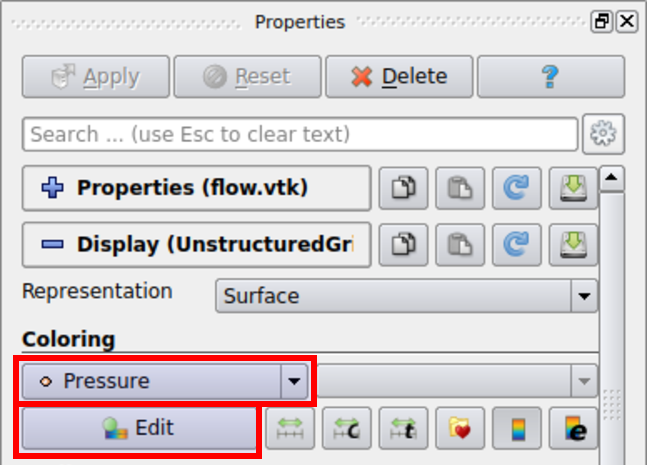
\includegraphics[width=0.4\textwidth]{tut02/pressurecont.pdf}
    \caption{Settings for displaying the pressure contour.}
    \label{fig2:pressure contours setting}
\end{figure}
Another display window will appear on the right-hand side of the monitor titled \textbf{Mapping Data}, similar to Figure \ref{fig2:color_range}.
\begin{figure}[htbp]
    \centering
    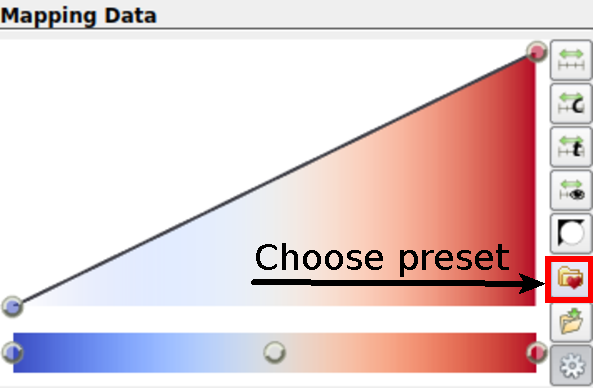
\includegraphics[width=0.4\textwidth]{tut02/colorrange.pdf}
    \caption{Changing color range for pressure contour.}
    \label{fig2:color_range}
\end{figure}
Now you can change contour colors by choosing \textbf{Choose preset}. Here, we select \textit{Cold and Hot} color range to be able to show clearly the sharp changes in pressure values around the shock (Figure \ref{fig2:color_range_item}). Then, click \textbf{Apply} for the next step.
\begin{figure}[htbp]
    \centering
    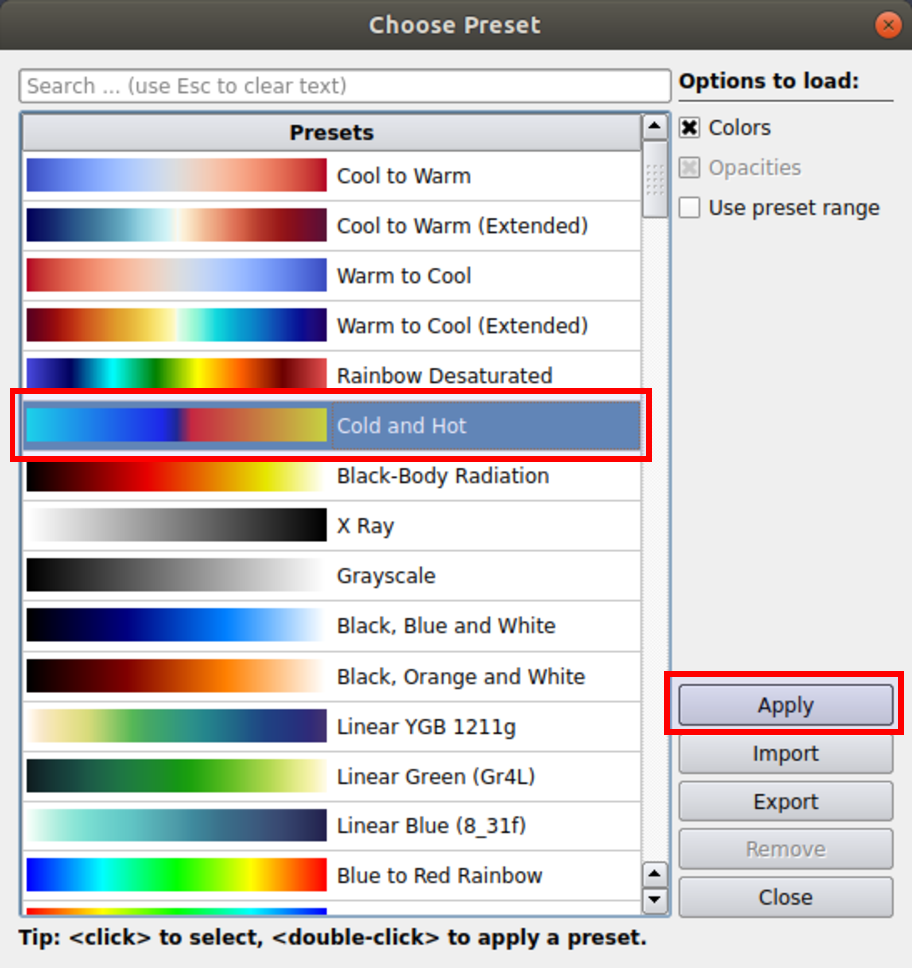
\includegraphics[width=0.5\textwidth]{tut02/changecontourcolors.pdf}
    \caption{Different color ranges to display contour.}
    \label{fig2:color_range_item}
\end{figure}
To add axes to the plots look under the \textbf{Miscellaneous} form of \textbf{Display} (Figure \ref{fig2:add axis}) and select the check box beside \textbf{Data Axes Grid}. Then go to \textbf{Edit} and change these options based on your preferences (Figure \ref{fig2:axis setting}).
\begin{figure}[htbp]
    \centering
    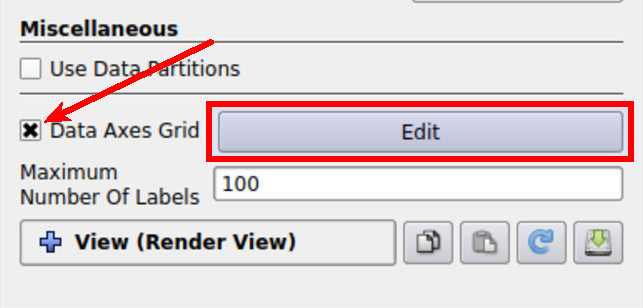
\includegraphics[width=0.4\textwidth]{tut02/addaxis.pdf}
    \caption{How to add axis to the plots.}
    \label{fig2:add axis}
\end{figure}
\begin{figure}[htbp]
    \centering
    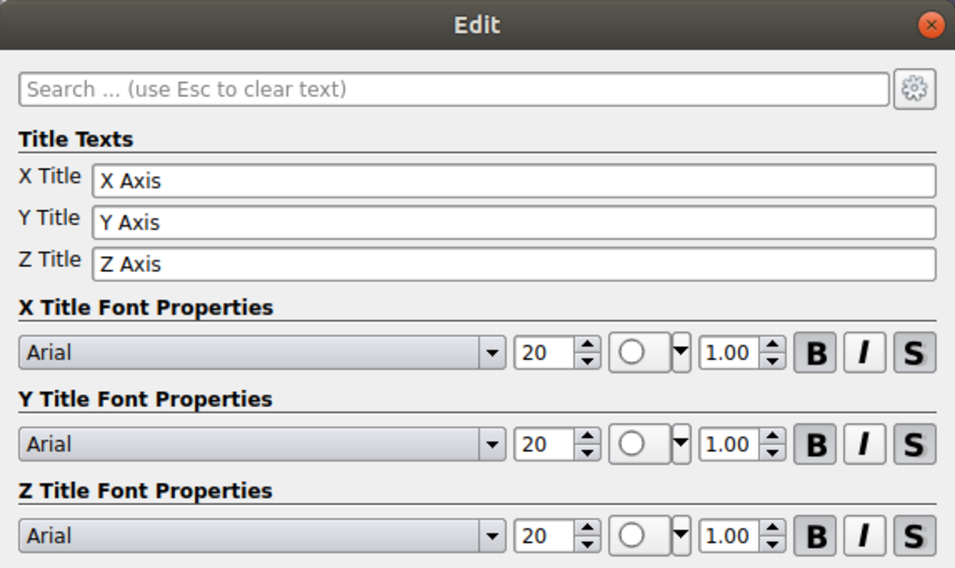
\includegraphics[width=0.6\textwidth]{tut02/axissettings.pdf}
    \caption{Settings for axis style.}
    \label{fig2:axis setting}
\end{figure}
Finally, the pressure contour you get should be similar to Figure \ref{fig2:plot pressure cont1}.
\begin{figure}[htbp]
    \centering
    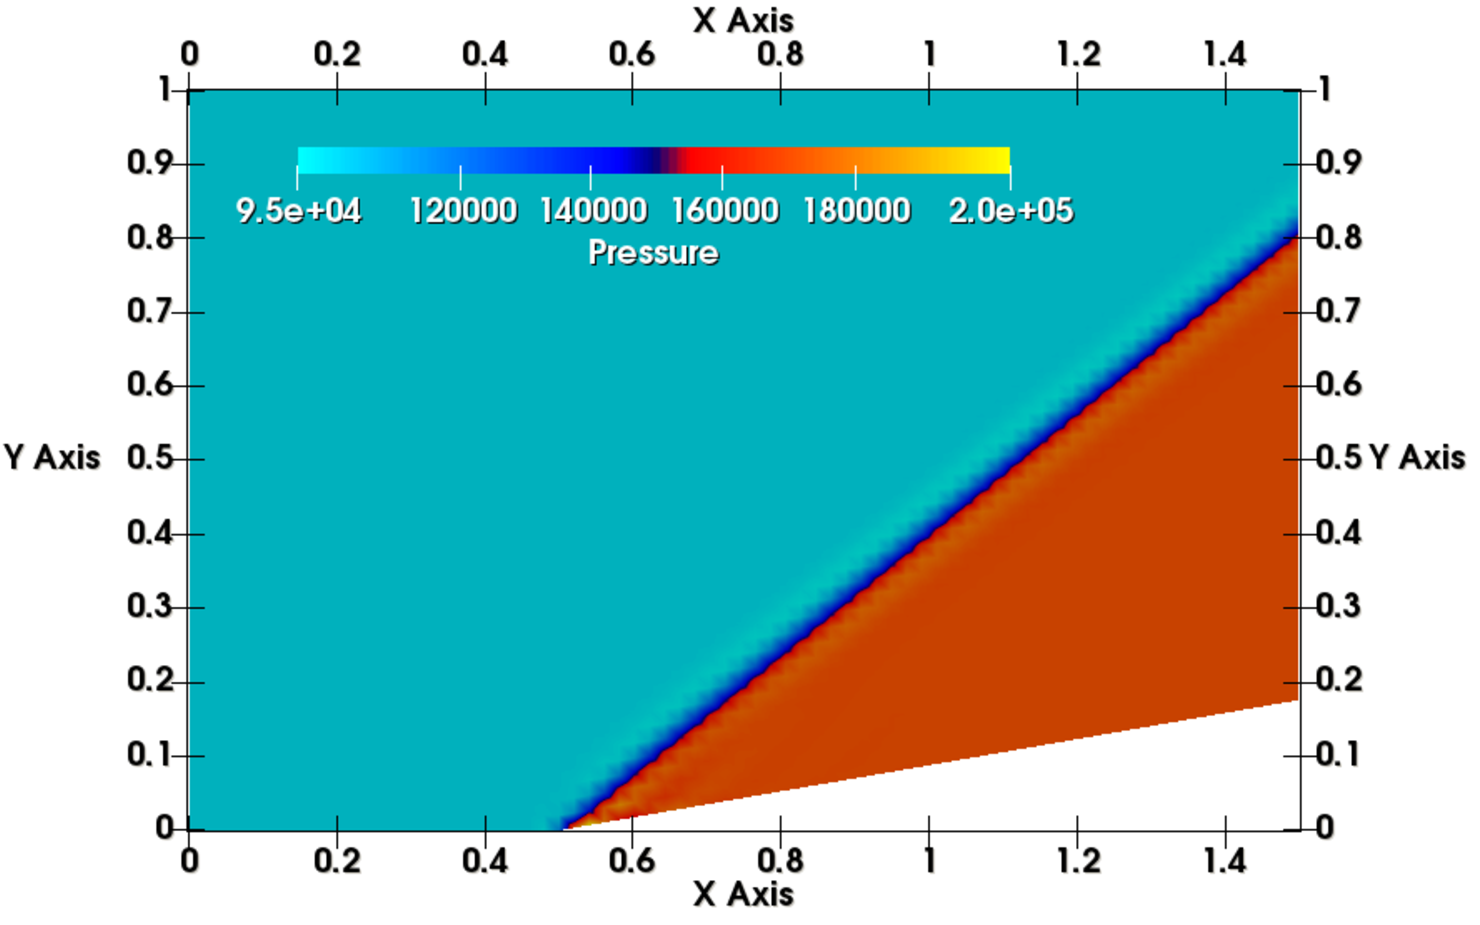
\includegraphics[width=0.85\textwidth]{tut02/plot1pressurecont.pdf}
    \caption{Pressure contour for supersonic wedge.}
    \label{fig2:plot pressure cont1}
\end{figure}
%----------------------------------------------------------

The pressure gradient along the shock wave is very difficult to see, and we want to add contour lines to
separate the different regions. To add contour lines, click again on the \textit{flow}.vtk file in the \textbf{Pipeline Browser}, and then click on the \textbf{Contour} icon (Figure \ref{fig2:contour_icon}) in toolbar.
\begin{figure}[htbp]
    \centering
    \includegraphics[width=0.5\textwidth]{tut02/contourlineicon.pdf}
    \caption{\textbf{Contour} icon in toolbar.}
    \label{fig2:contour_icon}
\end{figure}
Now the \textit{Contour1} item appears under \textit{flow}.vtk file in the \textbf{Pipeline Browser} (Figure \ref{fig2:contour1}). Click on \textbf{Apply} to proceed to the next step.
\begin{figure}[htbp]
    \centering
    \includegraphics[width=0.4\textwidth]{tut02/contour1.pdf}
    \caption{Adding \textit{Contour1} in \textbf{Pipeline Browser}.}
    \label{fig2:contour1}
\end{figure}
With regard to Figure \ref{fig2:contourby a}, go to the \textbf{Properties} tab, and select \textit{Pressure} from the \textbf{Contour By} drop-down menu. Next, click on the \textbf{Add Range} icon to customize the range to be used for the pressure contours. In Figure \ref{fig2:contourby b}, you will see the max/min range of contour lines (i.e. \textbf{From}/\textbf{To}), as well as number of lines you would like to have in your contour plot (i.e. \textbf{Steps}). Next, set \textbf{Steps} to 20, and click \textbf{OK}. By doing this the pressure contour range is equally divided into 20 lines. At the end, click on \textbf{Apply} to see contour lines in display window.
\begin{figure}[htbp]
    \centering
     \begin{subfigure}[b]{.4\textwidth}
         \centering
         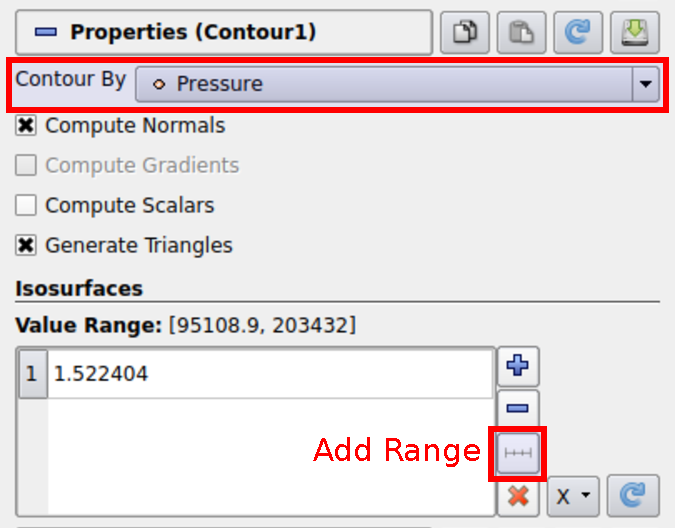
\includegraphics[width=1.0\textwidth]{tut02/contourby.pdf}
         \caption{Define new range}
         \label{fig2:contourby a}
     \end{subfigure}
     \hfill
     \begin{subfigure}[b]{.4\textwidth}
         \centering
         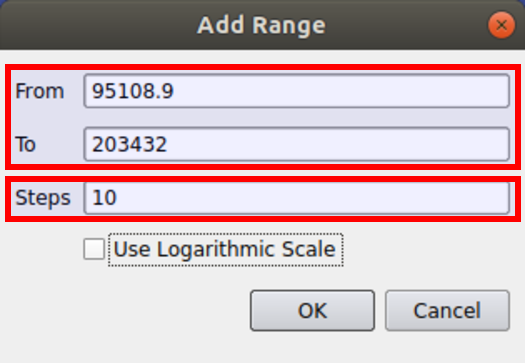
\includegraphics[width=1.0\textwidth]{tut02/addrange.pdf}
         \caption{Add range}
         \label{fig2:contourby b}
     \end{subfigure}     
    \caption{How to define a new range for the contour lines.}
    \label{fig2:contourby}
\end{figure}
Next, as it is shown in Figure \ref{fig2:colorby2}, click on the \textbf{Display} under \textbf{Properties} tab. In the \textbf{Coloring} section select \textbf{Solid Color} from the drop-down menu and choose white from \textbf{Edit}.
\begin{figure}[htbp]
    \centering
    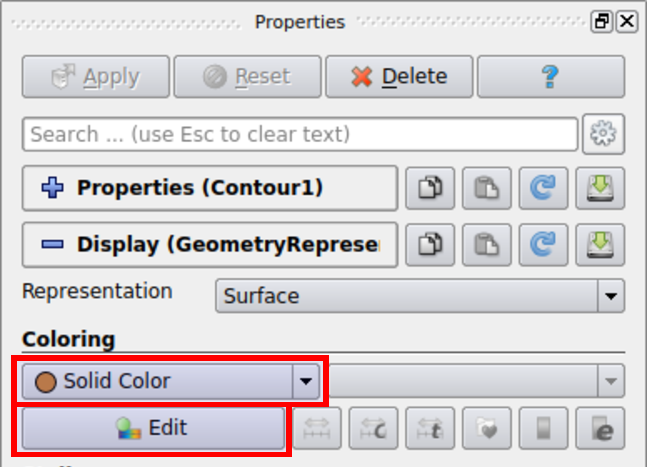
\includegraphics[width=0.4\textwidth]{tut02/contourline.pdf}
    \caption{Changing contour lines color in \textbf{Coloring} section.}
    \label{fig2:colorby2}
\end{figure}
The pressure contour lines should now be similar to Figure \ref{fig2:pressure_contour_lines}.
\begin{figure}[htbp]
    \centering
    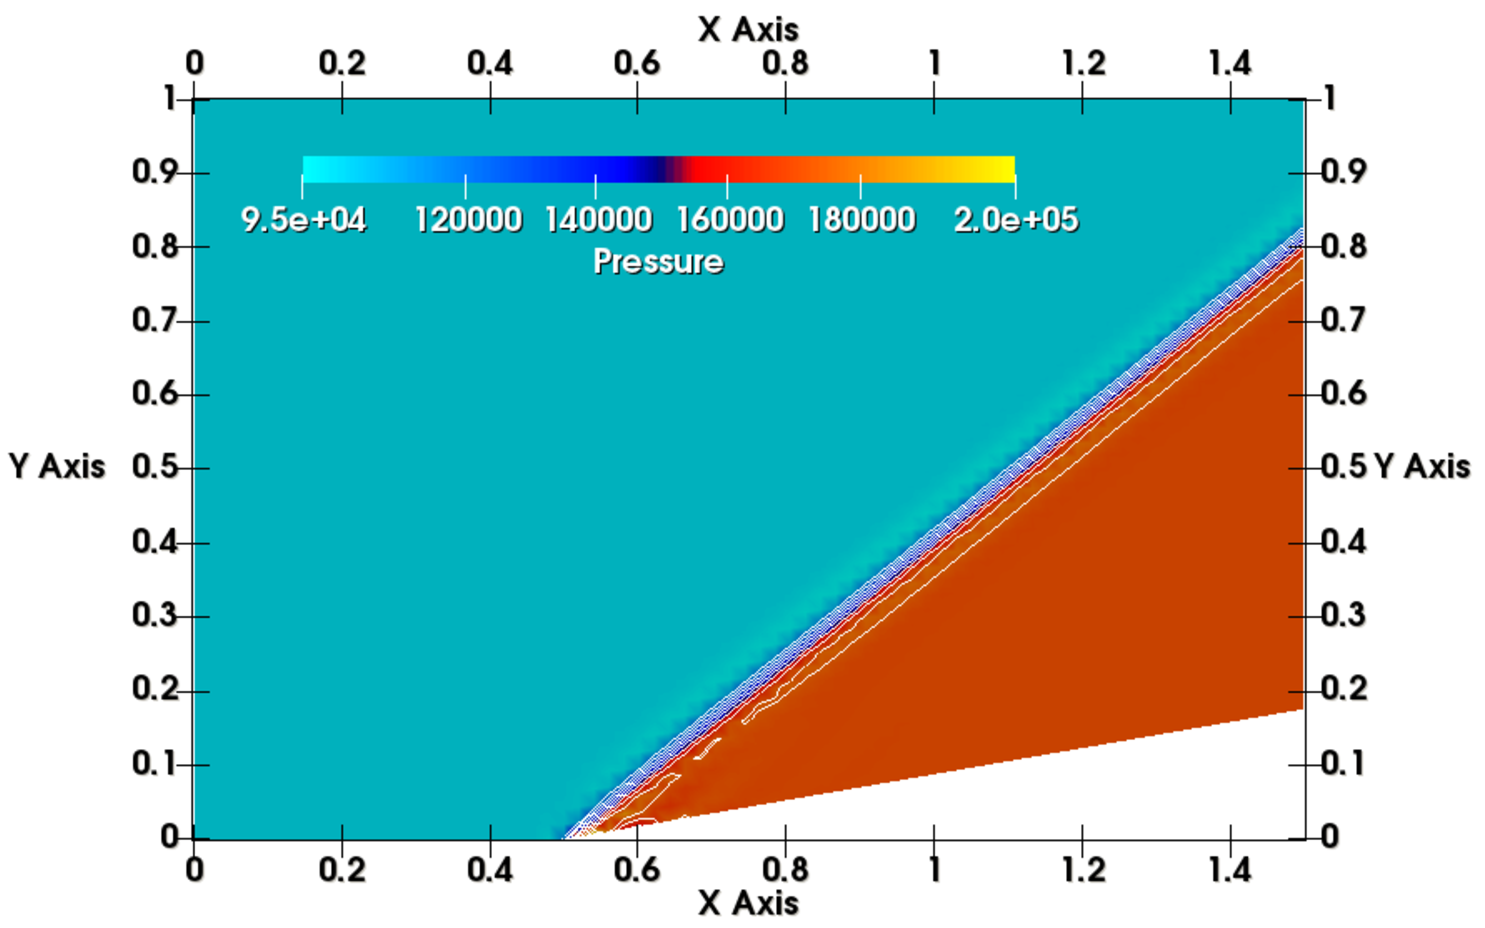
\includegraphics[width=.85\textwidth]{tut02/plot2pressurecont.pdf}
    \caption{Pressure contour superimposed by contour lines for supersonic wedge.}
    \label{fig2:pressure_contour_lines}
\end{figure}
You can zoom-in to the region at the bottom of the wedge to see the pressure gradient along the oblique
shock, as shown in Figure \ref{fig2:pressure_contour_lines_zoom}.
\begin{figure}[htbp]
    \centering
    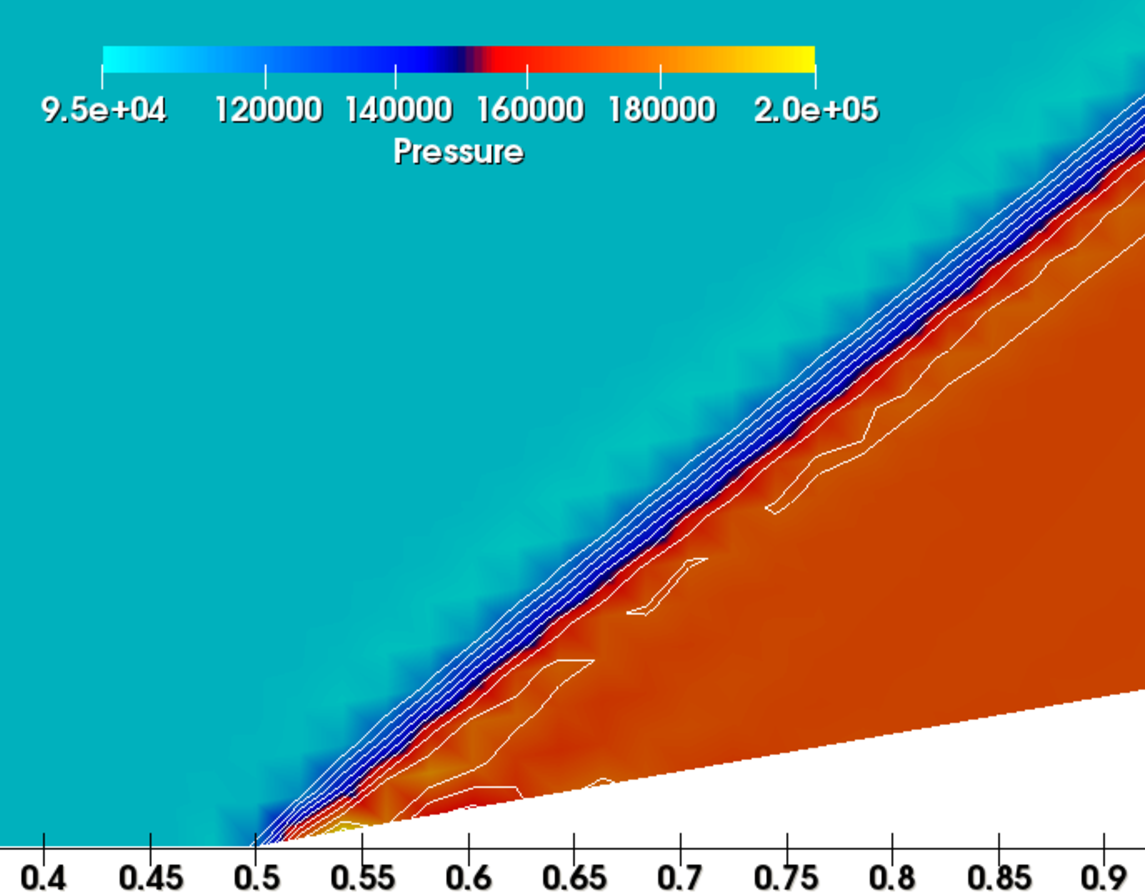
\includegraphics[width=.65\textwidth]{tut02/plot3pressurecont.pdf}
    \caption{Magnified pressure contour superimposed by contour lines for supersonic wedge.}
    \label{fig2:pressure_contour_lines_zoom}
\end{figure}

The other important plot we want to generate is related to the Mach number. To display the Mach number contours, click on \textit{flow}.vtk in the \textbf{Pipeline Browser}. Similar to Figure \ref{fig2:pressure contours setting}, under \textbf{Coloring} section, select \textit{Mach} from the drop-down menu. Next, click on \textit{Contour1} in the \textbf{Pipeline Browser}. Now, under \textbf{Properties} select \textit{Mach} from the \textbf{Contour By} drop-down menu. Since all these settings are related to the previous pressure value, we need to revise some options to display contours of \textit{Mach} number appropriately. To do this we need to delete the data range that was used for pressure, and replace it with the data range of that Mach number. Under \textbf{Isosurfaces} from \textbf{Properties}, click on the \textbf{Remove All} icon, and then click on the \textbf{Add Range} icon, as shown in Figure \ref{fig2:contourby2 a}. As you can see from Figure \ref{fig2:contourby2 b}, the max/min values for mach number has changed. Now set the \textbf{Steps} to 20 and click on \textbf{OK} to proceed to the next step.
\begin{figure}[htbp]
    \centering
     \begin{subfigure}[b]{.4\textwidth}
         \centering
         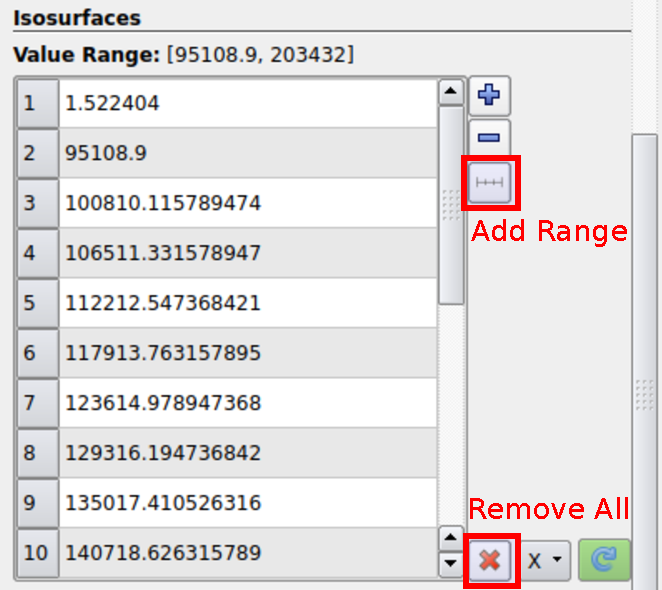
\includegraphics[width=1.0\textwidth]{tut02/deladdrange.pdf}
         \caption{Define new range}
         \label{fig2:contourby2 a}
     \end{subfigure}
     \hfill
     \begin{subfigure}[b]{.4\textwidth}
         \centering
         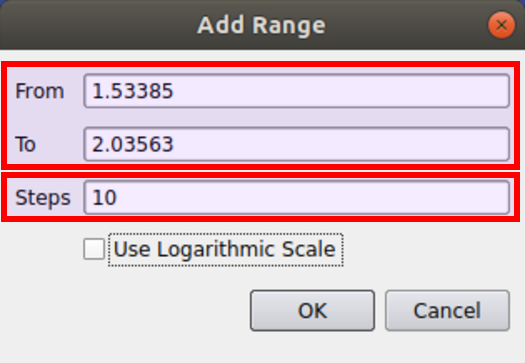
\includegraphics[width=1.0\textwidth]{tut02/addrange2.pdf}
         \caption{Add range}
         \label{fig2:contourby2 b}
     \end{subfigure}     
    \caption{How to define a new range for the contour lines.}
    \label{fig2:contourby2}
\end{figure}
Now the Mach number contour should look similar to Figure \ref{fig2:mach_contour}. Additionally, if you zoom-in the plot you will see more contour details near the wedge, similar to Figure \ref{fig2:mach_contour_zoom}.
\begin{figure}[htbp]
    \centering
    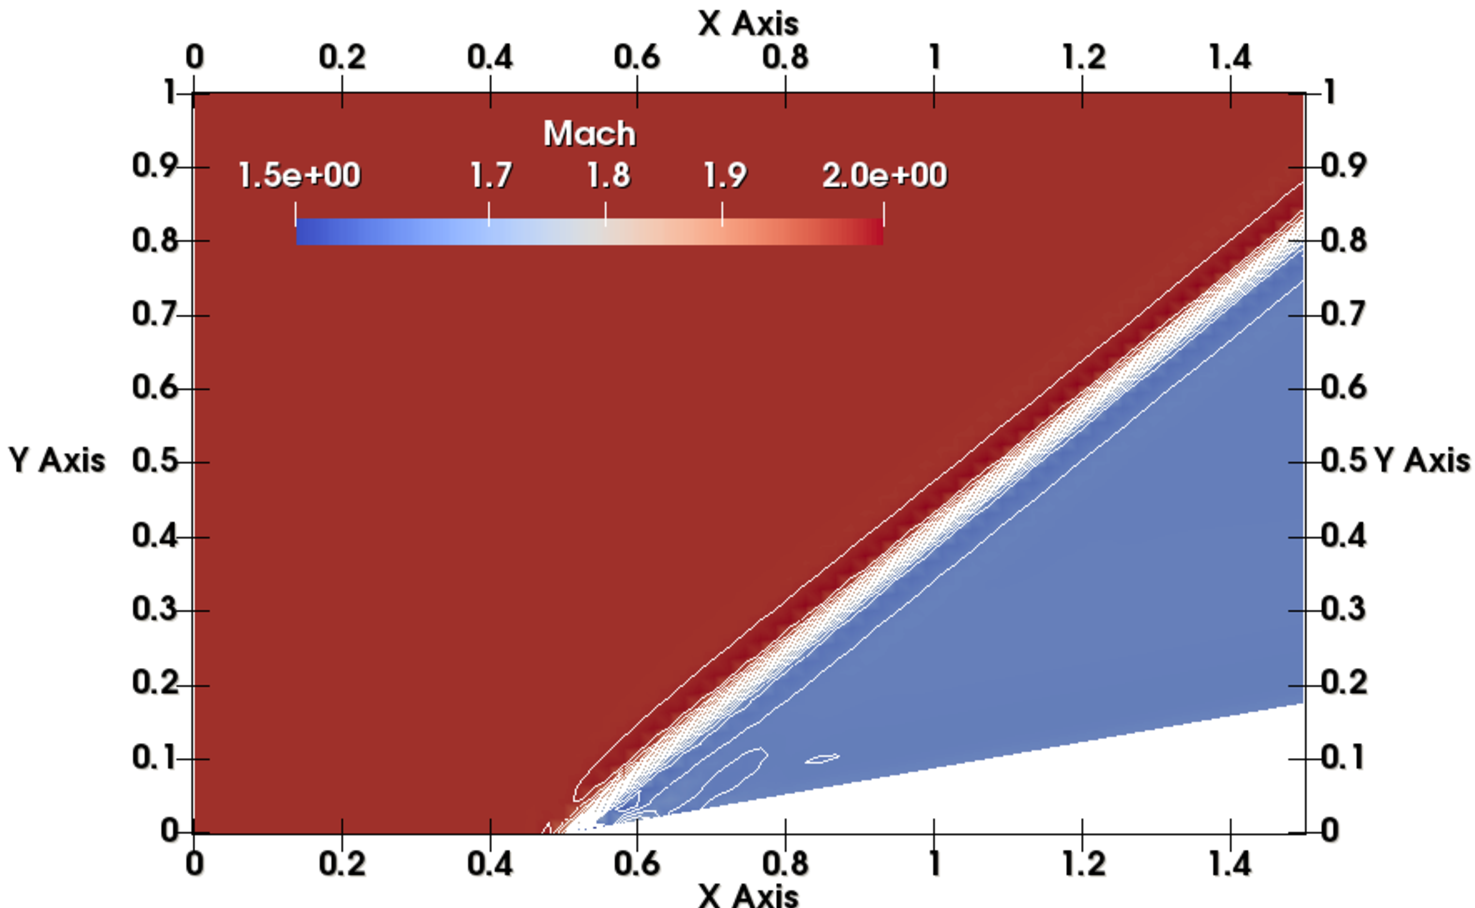
\includegraphics[width=.85\textwidth]{tut02/plot1machcont.pdf}
    \caption{Mach number contour superimposed by contour lines for supersonic wedge.}
    \label{fig2:mach_contour}
\end{figure}
\begin{figure}[htbp]
    \centering
    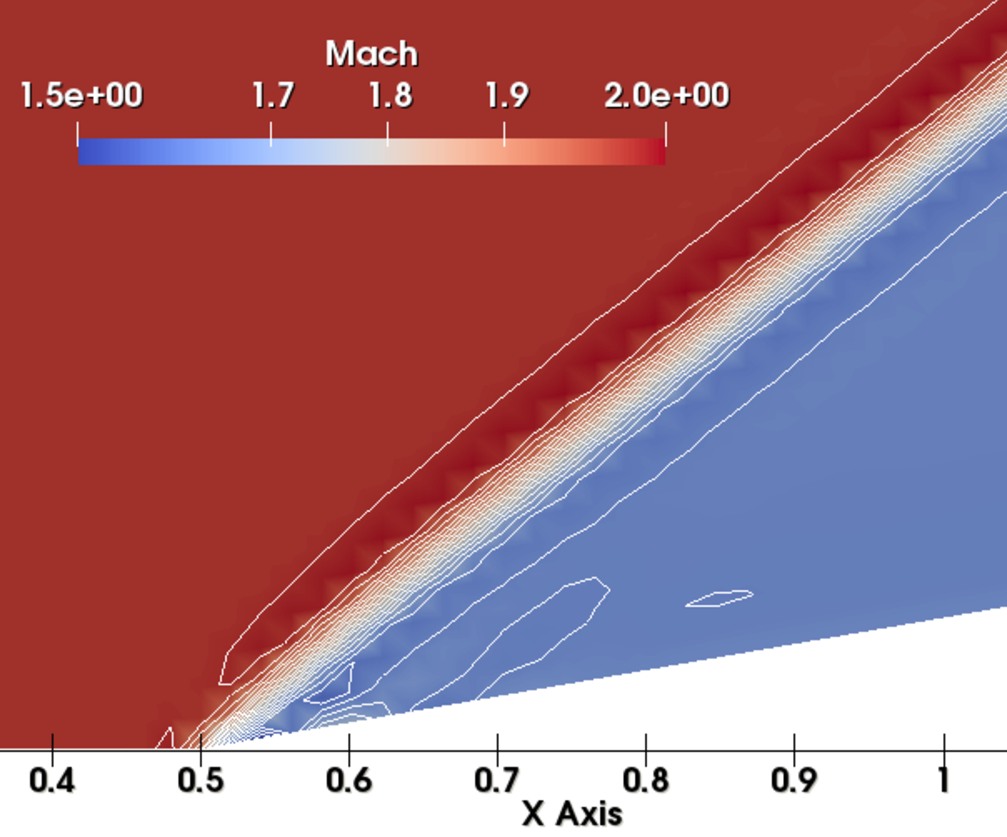
\includegraphics[width=.65\textwidth]{tut02/plot1machcont2.pdf}
    \caption{Magnified Mach number contour superimposed by contour lines for supersonic wedge.}
    \label{fig2:mach_contour_zoom}
\end{figure}
%--------------------------------------------------------------
\subsection{Plotting a variable over an arbitrary line}
To plot a variable over an arbitrary line, you can activate \textit{flow}.vtk by clicking on it in the \textbf{Pipeline Browser}. Next, as shown in Figure \ref{fig2:plot_over_line}, go to \textbf{Filters} $\rightarrow$  \textbf{Data Analysis} $\rightarrow$  \textbf{Plot Over Line}.
\begin{figure}[htbp]
    \centering
    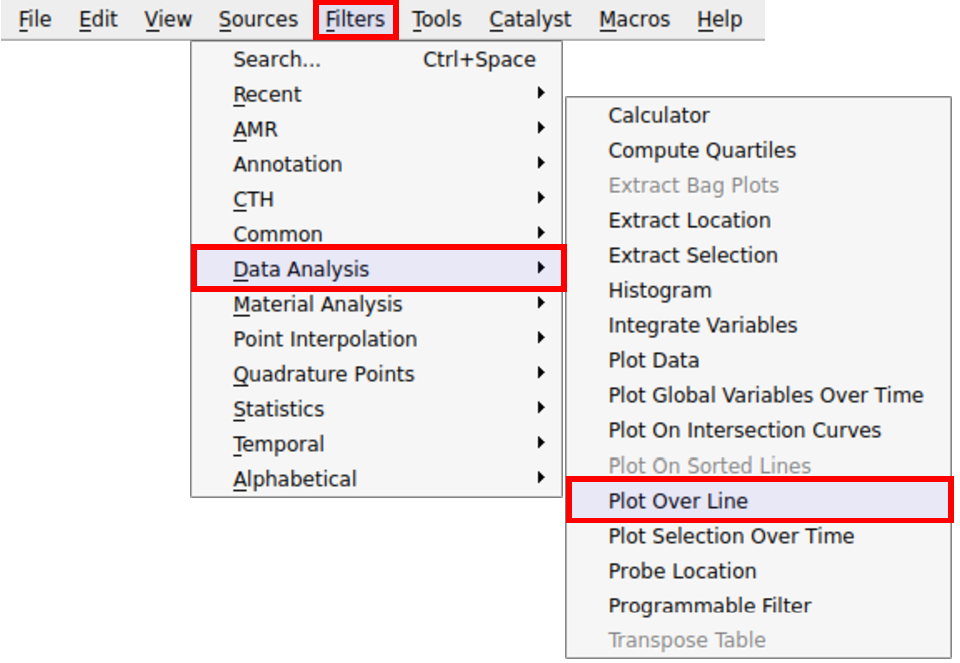
\includegraphics[width=.75\textwidth]{tut02/plotoverline.pdf}
    \caption{How to plot over an arbitrary line.}
    \label{fig2:plot_over_line}
\end{figure}
Next, as shown in Figure \ref{fig2:line_coordinate}, under \textbf{Line Parameters} in \textbf{Properties}, select the coordinates for two arbitrary points you want (i.e. \textbf{Point1} and \textbf{Point2}). In this case, plot the line from \textbf{Point1} to \textbf{Point2} with (0,0.5,0) and (1.5,0.5,0), respectively, and then click \textbf{Apply}.
\begin{figure}[htbp]
    \centering
    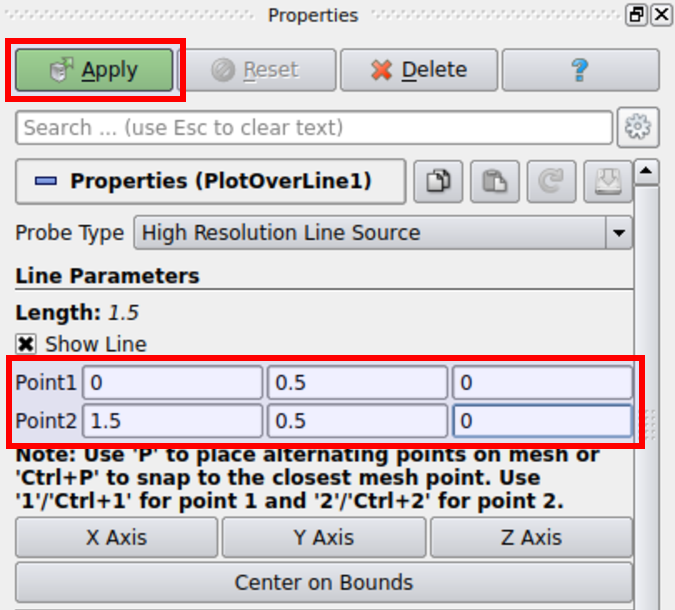
\includegraphics[width=.45\textwidth]{tut02/linecoord.pdf}
    \caption{Define the coordinates for plotting over the line.}
    \label{fig2:line_coordinate}
\end{figure}
A new line plot item will be generated. As shown in Figure \ref{fig2:plot_line_setting}, under the \textbf{X Axis Parameters} from \textbf{Display}, pick \textit{Point\_X} from the \textbf{X Array Name} drop-down menu. Now, under the \textbf{Series Parameters}, toggle the box beside \textbf{Variable} to uncheck everything, then select only the \textit{Mach} item.
\begin{figure}[htbp]
    \centering
    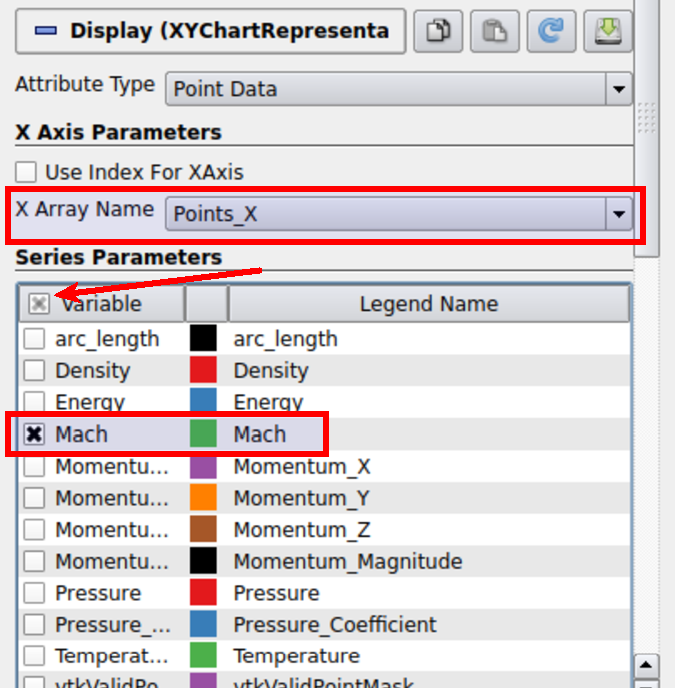
\includegraphics[width=.45\textwidth]{tut02/plotmachline.pdf}
    \caption{How to plot Mach number over a line.}
    \label{fig2:plot_line_setting}
\end{figure}
The plot of Mach number vs the \textit{x-coordinate} will be displayed in the main window as shown in Figure \ref{fig2:plot_line}.
\begin{figure}[htbp]
    \centering
    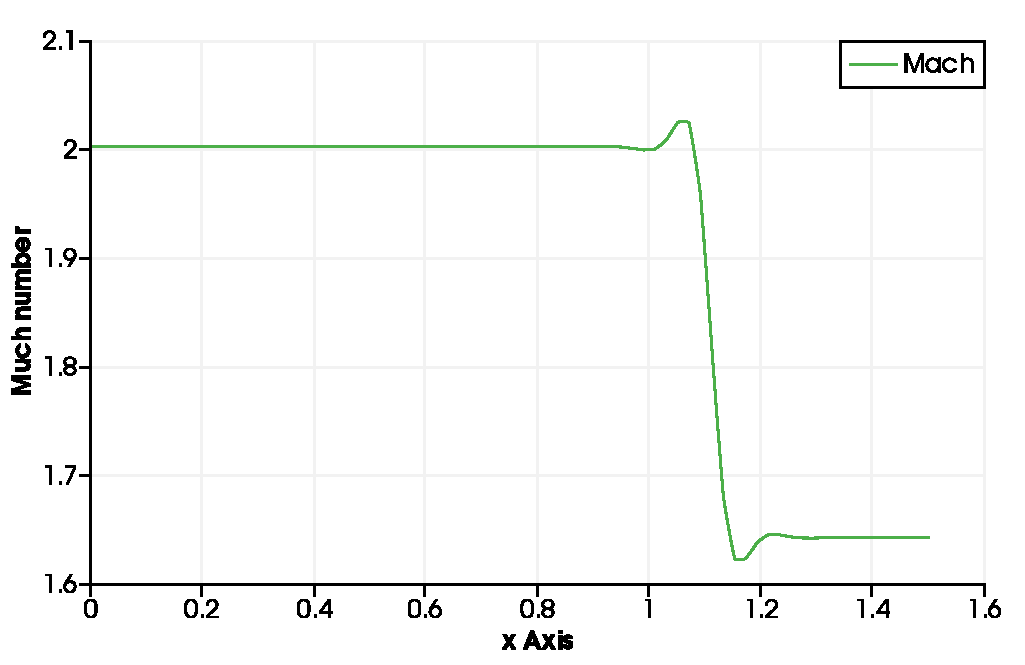
\includegraphics[width=.85\textwidth]{tut02/plot2contourline.pdf}
    \caption{Mach number plot over a specified line in \textit{x-coordinate}.}
    \label{fig2:plot_line}
\end{figure}
In order to see a spreadsheet view, click the upper right icon as shown in Figure \ref{fig2:open_spreadsheet}, then click on the \textit{Spreadsheet View} like Figure \ref{fig2:spreadsheet}.
\begin{figure}[htbp]
    \centering
    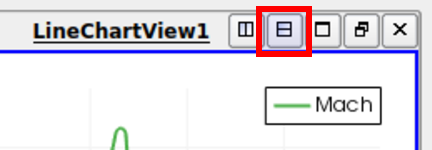
\includegraphics[width=.3\textwidth]{tut02/openspreadsheet.pdf}
    \caption{How to make spreadsheet view in a new window.}
    \label{fig2:open_spreadsheet}
\end{figure}
\begin{figure}[htbp]
    \centering
    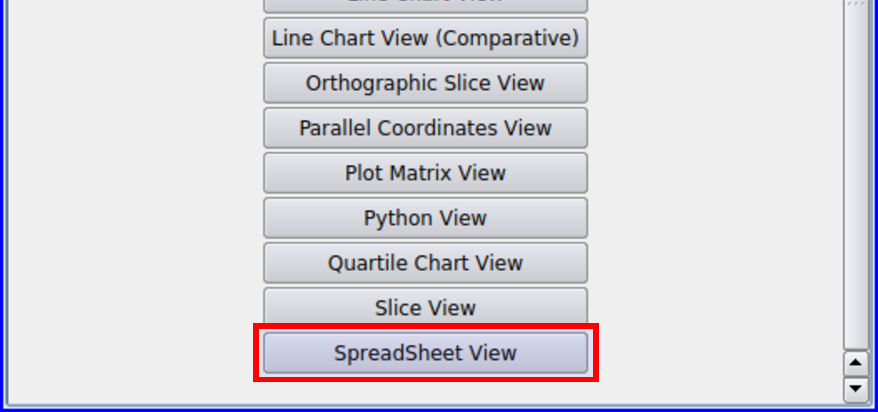
\includegraphics[width=.65\textwidth]{tut02/spreadsheet.pdf}
    \caption{Selecting \textit{Spreadsheet View} among different views.}
    \label{fig2:spreadsheet}
\end{figure}
Additionally, you can export a .csv file and plot it with any other plotting software. To export the spreadsheet as a .csv file, go to \textbf{File} $\rightarrow$ \textbf{Export}, and then \textbf{Save as} .csv.
%++++++++++++++++++++++++++++++++++++++++++++++++++++++++++++++
\clearpage
\section{Questions}
1. Run the default case as provided which uses 2ND\_ORDER and the HLLC Riemann solver.
\begin{enumerate}[label=(\alph*)]
    \item Create coloured contours of Pressure and Mach number in the entire domain.
    \item Plot Pressure from (0,0.5,0) to (1.5,0.5,0) using the \textbf{Plot Over Line}.
\end{enumerate}
2. Repeat Q.1 but switch the SPATIAL\_ORDER\_FLOW to 1ST\_ORDERs. \\
3. Repeat 1 using SPATIAL\_ORDER\_FLOW as 2ND\_ORDER but using the JST flux. \\
4. Repeat Q.1 using SPATIAL\_ORDER\_FLOW as 2ND\_ORDER but using the LAX-FRIEDRICH flux. \\
5. Repeat Q.1 using SPATIAL\_ORDER\_FLOW as 2ND\_ORDER but using the CUSP flux. \\
6. Repeat Q.1 using SPATIAL\_ORDER\_FLOW as 2ND\_ORDER but using the ROE flux. \\
7. Comment on how spatial order of accuracy and choice of Riemann solver affects the resolution of the shock and any dissipation or dispersion errors you can observe.
%++++++++++++++++++++++++++++++++++++++++++++++++++++++++++++++
%++++++++++++++++++++++++++++++++++++++++++++++++++++++++++++++
%++++++++++++++++++++++++++++++++++++++++++++++++++++++++++++++
\chapter{Inviscid ONERA M6}
\label{ch:Inviscid ONERA M6}
%++++++++++++++++++++++++++++++++++++++++++++++++++++++++++++++
\section{Problem Description}
In this tutorial, we are going to explain how to simulate external, compressible, and transonic inviscid flow past a 3D wing. The chosen wing is ONERA M6 which is a well-known CFD test case for supersonic flows. This wing was designed by ONERA Aerodynamics Department as a bench mark for experimental studies. Due to availability of experimental data and simple geometry of wing, this wing has also attracted the attention of CFD engineers. Furthermore, CFD analysis of ONERA M6 wing is notable, since some of important phenomena occurs in this case, like transonic-shock, flow separation over the wing, 3D structure of flow around the tip of the wing. In this tutorial, the computational domain with unstructured mesh consists of 582,752 tetrahedral elements and 108,396 nodes. For this example, the flow specifications are provided as follows:
\begin{itemize}
    \item Pressure = 101,325 Pa
    \item Temperature = 273.15 K
    \item Mach number = 0.8395
    \item angle of attack = 3.06 degrees
\end{itemize}

The tutorial has two parts: Flow Solution and Post-processing. In the first part, we explain how to manage prerequisite files and settings, and how to run the CFD simulation using SU2. In the second part, we explain how to use Paraview software to visualize data obtained form SU2.
%++++++++++++++++++++++++++++++++++++++++++++++++++++++++++++++
\section{Flow solution}
In the configuration file, you can specify the multi-grid parameters. For the tutorial case, you will see that \texttt{MGLEVEL=0}. However, you can choose different level for your multi-grid method by giving an integer number to \texttt{MGLEVEL}. You can also select type of multi-grid cycle by setting one of existing options in \texttt{MGCYCLE (V Cycle, W Cycle or Full MG Cycle)}. Another parameter of interest is the total number of iterations. This can be modified by changing the value in \texttt{EXT\_ITER}. For this example it will be kept at 200 for brevity; but depending on the method used, higher iteration numbers may be necessary before solution can converge. In this tutorial, we want to look at the pressure coefficient and Mach number contours, solve for the lift coefficient ($C_L$) and drag coefficient ($C_D$) of the ONERA M6 wing, as well as observe the rate of convergence. This helps you to get to know how to speed up your simulation using multi-grid technique, and how to check convergence rate to assure your results are converged.

To run the simulation, the SU2 needs two essential files: configuration file (.cfg) and mesh file (.su2). In this example, the following files are located in \textit{03InviscidOneraM6} folder:
\begin{enumerate}
\item \textit{inv\_ONERAM6}.cfg as a configuration file.
\item \textit{mesh\_ONERAM6\_inv}.su2 as a mesh file.
\end{enumerate}
The next step is to copy these two files in directory of SU2, where the execution and script files are located there. To run this simulation, open the command line terminal and enter the following commands:
\begin{table}[htbp]
    \centering
    \begin{tabular}{|l|l|}
    \hline
    Windows     & \begin{tabular}{c} \$ cd "where you saved the package" \\ \$ SU2\_CFD.exe inv\_ONERAM6.cfg \end{tabular}
    \\
    \hline
    OSX     & \begin{tabular}{c} \$ cd "where you saved the package" \\ \$ SU2\_CFD.exe inv\_ONERAM6.cfg \end{tabular}
    \\
    \hline
    \end{tabular}
\end{table}

The SU2 solver will commence calculation and print out the residuals at every iteration until the specified convergence criteria is achieved. After calculations are done, the following output files should be generated and saved in the SU2 folder:
\begin{itemize}
    \item \textit{flow}.vtk: contains the full volume flow solution.
    \item \textit{force\_breakdown}.dat: contains forces and moment on the surface of the wing.
    \item \textit{history}.vtk: contains convergence history of calculations.
    \item \textit{restart\_flow}.dat: for restarting simulation.
    \item \textit{surface\_flow}.vtk: flow solution on the surface of the wing.
    \item \textit{surface\_flow}.csv: comma separated values of flow solution on the surface of the wing (If you want to plot data in another software, like Microsoft Excel, you can use this file).
\end{itemize}
Please keep in mind that every time you run SU2, the output data will be overwritten. Hence, before launching new simulation, you could make a new folder and transfer your data from previous simulation to this folder.
%++++++++++++++++++++++++++++++++++++++++++++++++++++++++++++++
\section{Post-processing}
In this section, we explain how to use Paraview to visualize CFD data for this example. First of all, install Paraview (this tutorial uses Paraview 3.12.0) if you do not have it on your computer. Otherwise, take following steps for visualization:
%--------------------------------------------------------------
\subsection{Load Solution File:}
Launch Paraview. Go to \textbf{File} $\rightarrow$ \textbf{Open}, and then select \textit{surface\_flow}.vtk file. On the left-hand side of Paraview window you will see the file appears under \textbf{builtin} in \textbf{Pipeline Browser}. Now press \textbf{Apply} button in \textbf{Properties} tab, just right under the  \textbf{Pipeline Browser}. After taking these steps, your file is loaded by software and is ready to visualize (Fig.\ref{fig3:load}).
\begin{figure}[htbp]
    \centering
    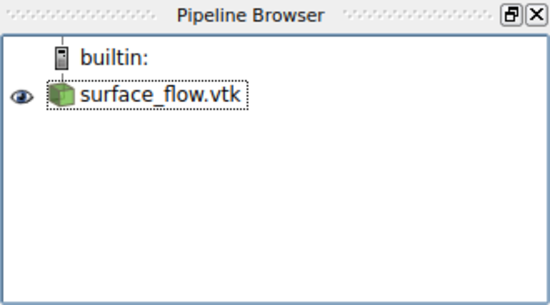
\includegraphics[width=0.4\textwidth]{tut03/surface_flow.pdf}
    \caption{Loading \textit{surface\_flow}.vtk file in the \textbf{Pipeline Browser}.}
    \label{fig3:load}
\end{figure}
%--------------------------------------------------------------
\subsection{Visualize Mesh Domain}
In order to view mesh, according to Fig.\ref{fig3:wireframe}, select \textit{Solid Color} with \textit{Wireframe} in the toolbar. As you can see from Fig.\ref{fig3:mesh}, the mesh around the ONERA M6 wing is unstructured, and the grids are clustered around the tip, leading and trailing edges of the wing. The reason for this clustering is that the changes in flow variables are high at these regions and the mesh should be fine enough at vicinity of these regions in order to solve flow accurately.
\begin{figure}[htbp]
    \centering
    \includegraphics[width=0.6\textwidth]{tut03/wireframe.pdf}
    \caption{How to display mesh in computational domain.}
    \label{fig3:wireframe}
\end{figure}
\begin{figure}[htbp]
    \centering
    \includegraphics[width=.75\textwidth]{tut03/mesh2.pdf}
    \caption{Unstructured mesh around ONERA M6 wing.}
    \label{fig3:mesh}
\end{figure}
%--------------------------------------------------------------
\subsection{Visualize Pressure Coefficient Contour and Much Number Contour}
To display the pressure contour, click on the \textit{surface\_flow}.vtk in the \textbf{Pipeline Browser}, and then click on the \textbf{Display} in \textbf{Properties} tab. Next, under \textbf{Coloring}, select \textit{Pressure\_Coefficient} from drop-down menu (Fig.\ref{fig3:pressure_coeff_1}).
\begin{figure}[htbp]
    \centering
    \includegraphics[width=0.4\textwidth]{tut03/coloring.pdf}
    \caption{Display contour by selecting variable.}
    \label{fig3:pressure_coeff_1}
\end{figure}
Eventually, the pressure coefficient contour should be similar to Fig.\ref{fig3:plot_pressure_coeff}
\begin{figure}[htbp]
    \centering
    \includegraphics[width=0.65\textwidth]{tut03/cont1_pressure_coefficient.pdf}
    \caption{Pressure coefficient contour for ONERA M6 wing.}
    \label{fig3:plot_pressure_coeff}
\end{figure}

In order to add contour lines to the plot, click again on the \textit{surface\_flow}.vtk in the \textbf{Pipeline Browser}, and then click on the \textbf{Contour} icon (Fig.\ref{fig3:contour_icon}) in toolbar.
\begin{figure}[htbp]
    \centering
    \includegraphics[width=0.5\textwidth]{tut03/contourlineicon.pdf}
    \caption{\textbf{Contour} icon in toolbar.}
    \label{fig3:contour_icon}
\end{figure}
Eventually, \textit{Contour1} appears under \textit{flow}.vtk file in the \textbf{Pipeline Browser} (Fig.\ref{fig3:contour1}). Then, click on \textbf{Apply} to proceed next step.
\begin{figure}[htbp]
    \centering
    \includegraphics[width=0.4\textwidth]{tut03/contour1.pdf}
    \caption{Adding \textit{Contour1} in \textbf{Pipeline Browser}.}
    \label{fig3:contour1}
\end{figure}
According to Fig.\ref{fig3:contourby a}, go to the \textbf{Properties}, and choose \textit{Pressure\_Coefficient} from \textbf{Contour By} drop-down menu. Then, click on the \textbf{Add Range} icon to customize the range of pressure contour. As seen from Fig.\ref{fig3:contourby b},  max/min (i.e. \textbf{From}/\textbf{To}) range of contour lines, as well as the number steps required to divide this range into the equal portions exist. So, set \textbf{Step} to 20, and click on \textbf{OK}. At the end, click on \textbf{Apply} to illustrate contour lines in display window.
\begin{figure}[htbp]
    \centering
     \begin{subfigure}[b]{.4\textwidth}
         \centering
         \includegraphics[width=1.0\textwidth]{tut03/pressure_coeff_addrange1.pdf}
         \caption{Define new range}
         \label{fig3:contourby a}
     \end{subfigure}
     \hfill
     \begin{subfigure}[b]{.4\textwidth}
         \centering
         \includegraphics[width=1.0\textwidth]{tut03/pressure_coeff_addrange2.pdf}
         \caption{Add range}
         \label{fig3:contourby b}
     \end{subfigure}     
    \caption{How to define a new range for the contour lines.}
    \label{fig3:contourby}
\end{figure}
Next, as it is shown in Fig.\ref{fig3:colorby2}, click on the \textbf{Display} under \textbf{Properties} tab. In \textbf{Coloring} section, select \textbf{Solid Color} form drop-down menu, and choose black color from \textbf{Edit}.
\begin{figure}[htbp]
    \centering
    \includegraphics[width=0.4\textwidth]{tut03/coloring2.pdf}
    \caption{Changing contour lines color in \textbf{Coloring} section.}
    \label{fig3:colorby2}
\end{figure}
Eventually, the pressure contour with black contour lines should be similar to Fig.\ref{fig3:pressure_contour_lines}.
\begin{figure}[htbp]
    \centering
    \includegraphics[width=.65\textwidth]{tut03/cont2_pressure_coefficient.pdf}
    \caption{Pressure coefficient contour superimposed by contour lines for ONERA M6 wing.}
    \label{fig3:pressure_contour_lines}
\end{figure}

To display the Mach number contour, similar to Fig.\ref{fig3:pressure_coeff_1}, click on the \textit{surface\_flow}.vtk in the \textbf{Pipeline Browser}, and under \textbf{Coloring} from \textbf{Display}, select \textit{Mach} from drop-down menu. In the next step, click on "\textit{Contour1}" in the \textbf{Pipeline Browser}. As it is shown in Fig.\ref{fig3:contourby2 a}, under \textbf{Properties}, select \textit{Mach} from \textbf{Contour By} drop-down menu. Next, click on \textbf{Remove All} icon to remove previous value range belonged to pressure coefficient. Similar to Fig.\ref{fig3:contourby2 b}, click on \textbf{Add Range} icon and set \textbf{Steps} to 20. Next, click on \textbf{OK}, and then, \textbf{Apply} to show plot.
\begin{figure}[htbp]
    \centering
     \begin{subfigure}[b]{.4\textwidth}
         \centering
         \includegraphics[width=1.0\textwidth]{tut03/del_add_range_mach.pdf}
         \caption{Define new range}
         \label{fig3:contourby2 a}
     \end{subfigure}
     \hfill
     \begin{subfigure}[b]{.4\textwidth}
         \centering
         \includegraphics[width=1.0\textwidth]{tut03/AddRangemach.pdf}
         \caption{Add range}
         \label{fig3:contourby2 b}
     \end{subfigure}     
    \caption{How to define a new range for the contour lines.}
    \label{fig3:contourby2}
\end{figure}
Now the Mach number contour of the wing surface should be similar to Fig.\ref{fig3:mach_contour}.
\begin{figure}[htbp]
    \centering
    \includegraphics[width=0.5\textwidth]{tut03/machcontour1.pdf}
    \caption{Mach number contour with superimposed by lines.}
    \label{fig3:mach_contour}
\end{figure}
%--------------------------------------------------------------
\subsection{Comparison of Convergence Rate}
Launch Microsoft Excel or any other plotting software. For Microsoft Excel, open the file \textit{history}.vtk from the tutorial folder. Then, you are asked to choose the file type that best describes your data. You should select \textbf{Delimiters}, and in the next step, Under the \textbf{Delimiters}, select only the check boxes for \textit{Tab}, \textit{Semicolon}, and \textit{Comma} (Fig.\ref{fig3:importvtkxlxs}).
\begin{figure}[htbp]
    \centering
    \includegraphics[width=0.5\textwidth]{tut03/16.png}
    \caption{Import .vtk file in Microsoft Excel.}
    \label{fig3:importvtkxlxs}
\end{figure}
As shown in Fig.\ref{fig3:columnsxlxs}, the first column shows the iteration number. The lift coefficient ($C_L$) and the drag coefficient ($C_D$) are displayed in the second and third column, respectively. Additionally, the residuals can also be examined to check convergence (Column \textit{L} to Column \textit{P} in Fig.\ref{fig3:residualxlxs}).
\begin{figure}[htbp]
    \centering
    \includegraphics[width=0.5\textwidth]{tut03/17.png}
    \caption{Columns in \textit{history}.vtk}
    \label{fig3:columnsxlxs}
\end{figure}
\begin{figure}[htbp]
    \centering
    \includegraphics[width=0.75\textwidth]{tut03/18.png}
    \caption{Residuals in \textit{history}.vtk}
    \label{fig3:residualxlxs}
\end{figure}
Now we plot the lift coefficient, drag coefficient, and density residual against the number of iterations to see how many iterations it takes to converge to a steady solution. Fig.\ref{fig3:clcdxlxs} and Fig.\ref{fig3:res_vs_itr} shows the plots for aerodynamic loads and residual versus the number of iterations, respectively, for the case of \texttt{MGLEVEL=0} on tetrahedral mesh.
\begin{figure}[htbp]
    \centering
    \includegraphics[width=0.75\textwidth]{tut03/22.png}
    \caption{Lift and Drag coefficients versus the number of iterations.}
    \label{fig3:clcdxlxs}
\end{figure}
\begin{figure}[htbp]
    \centering
    \includegraphics[width=0.75\textwidth]{tut03/21.png}
    \caption{Density residual versus the number of iterations.}
    \label{fig3:res_vs_itr}
\end{figure}
%++++++++++++++++++++++++++++++++++++++++++++++++++++++++++++++
\section{Questions}
1. Run the simulation without multi-grid scheme (\texttt{MGLEVEL=0}).
\begin{enumerate}[label=(\alph*)]
    \item Follow the procedure in the guideline document to run the simulation and record the number of iterations and wall-clock time for the simulation to complete.
    \item Record the lift and drag coefficients.
    \item Plot the surface pressure coefficient with coloured contours and contour lines.
    \item Plot the surface Mach number with coloured contours and contour lines.
    \item Plot the value of $C_L$, $C_D$ and the density residual vs. the number of iterations.
\end{enumerate}
2. Modify the configuration file in the multi-grid folder (\texttt{MGLEVEL= 3, MGCYCLE= W\_CYCLE}) and repeat Q.1 using multi-grid scheme.\\
3. Compare the results in part (a)-(e) of Q.1 and Q.2. In what way is the use of multi-grid advantageous for this test case?\\
%++++++++++++++++++++++++++++++++++++++++++++++++++++++++++++++
%++++++++++++++++++++++++++++++++++++++++++++++++++++++++++++++
%++++++++++++++++++++++++++++++++++++++++++++++++++++++++++++++
\chapter{Laminar Cylinder}
\label{ch:Laminar Cylinder}
%++++++++++++++++++++++++++++++++++++++++++++++++++++++++++++++
\section{Problem Description}
In this tutorial, we are going to explain how to simulate the external flow past a 2D cylinder. To simulate viscous flow, Navier-Stokes equations are solved in steady or unsteady format, depending at Reynolds numbers. According to observations, the flow remains symmetric and steady for Reynolds number less than around 46, while at higher Reynolds number the flow becomes unstable and asymmetric. Therefore, in this time-dependent flow,  Von-Karman Streets appear, which is a well-known phenomenon in fluid mechanics. The Von-Karman Streets correspond to pair vortex shedding behind the cylinder, where vortices are generated due to flow unsteadiness and disturbances. The computational domain for this tutorial is an O-topology domain with a cylinder in the center of the domain. The outer boundary is 15$D$ (where, $D$ is cylinder diameter) far away from the cylinder to reduce the outer boundary effect on the solution. The mesh includes 26,192 triangular elements and 13,336 points. The grids around the surface of the cylinder are fine since we want to solve the flow properly in the boundary layer. Keep in mind that since the viscous flow is solved, the flow near the wall boundaries are significantly important, and the velocity profile in the boundary layer should be captured appropriately. For this example, the flow specifications are provided as follows:
\begin{itemize}
    \item Pressure = 101,325Pa
    \item Temperature = 273.15K
    \item Mach number = 0.1
    \item angle of attack = 0 degrees
    \item Reynolds number = 40
    \item Characteristic length = 1m
\end{itemize}
The tutorial has two parts: Flow Solution and Post-processing. In the first part, we explain how to manage prerequisite files and settings, and then, how to run the CFD simulation using SU2. In the second part, we explain how to use Paraview software to visualize data obtained form SU2.
%++++++++++++++++++++++++++++++++++++++++++++++++++++++++++++++
\section{Flow solution}
To run the simulation, the SU2 needs two essential files: configuration file (.cfg) and mesh file (.su2). In this example, the following files are located in \textit{04LaminarCylinder} folder:
\begin{enumerate}
    \item lam\_cylinder.cfg as a configuration file.
    \item mesh\_cylinder\_lam.su2 as a mesh file.
\end{enumerate}
The next step is to copy these two files in directory of SU2, where the execution and script files are located there. To run this simulation, open the command line terminal and enter the following commands:
\begin{table}[htbp]
    \centering
    \begin{tabular}{|l|l|}
    \hline
    Windows     & \begin{tabular}{c} \$ cd "where you saved the package" \\ \$ SU2\_CFD.exe lam\_cylinder.cfg \end{tabular}
    \\
    \hline
    OSX     & \begin{tabular}{c} \$ cd "where you saved the package" \\ \$ SU2\_CFD.exe lam\_cylinder.cfg \end{tabular}
    \\
    \hline
    \end{tabular}
\end{table}

The SU2 solver will commence calculation and print out the residuals at every iteration until the specified convergence criteria is achieved. After calculations are done, the following output files should be generated and saved in the SU2 folder:
\begin{itemize}
    \item \textit{flow}.vtk: contains the full volume flow solution.
    \item \textit{force\_breakdown}.dat: contains forces and moment on the surface of the cylinder.
    \item \textit{history}.vtk: contains convergence history of calculations.
    \item \textit{restart\_flow}.dat: for restarting simulation.
    \item \textit{surface\_flow}.vtk: flow solution on the surface of the cylinder.
    \item \textit{surface\_flow}.csv: comma separated values of flow solution on the surface of the cylinder (If you want to plot data in another software, like Microsoft Excel, you can use this file).
\end{itemize}
Please keep in mind that every time you run SU2, the output data will be overwritten. Hence, before launching new simulation, you could make a new folder and transfer your data from previous simulation to this folder.
%++++++++++++++++++++++++++++++++++++++++++++++++++++++++++++++
\section{Post-processing}
In this section, we explain how to use Paraview to visualize CFD data for this example. First of all, install Paraview (this tutorial uses Paraview 3.12.0) if you do not have it on your computer. Otherwise, take following steps for visualization:
%--------------------------------------------------------------
\subsection{Load Solution File:}
Launch Paraview. Go to \textbf{File} $\rightarrow$ \textbf{Open}, and then select \textit{flow}.vtk file. On the left-hand side of Paraview window you will see the file appears under \textbf{builtin} in \textbf{Pipeline Browser}. Now press \textbf{Apply} button in \textbf{Properties} tab, just right under the \textbf{Pipeline Browser}. After taking these steps, your file is loaded by software and is ready to visualize (Fig.\ref{fig4:load}).
\begin{figure}[htbp]
    \centering
    \includegraphics[width=0.4\textwidth]{tut04/loadvtkfile.pdf}
    \caption{Loading \textit{flow}.vtk file in the \textbf{Pipeline Browser}.}
    \label{fig4:load}
\end{figure}
%--------------------------------------------------------------
\subsection{Visualize Mesh Domain}
In order to display mesh used as computational domain, according to Fig.\ref{fig4:wireframe_4}, select \textit{Solid Color} with \textit{Wireframe} in the toolbar. Then, you can zoom-in to see mesh around the cylinder like Fig.\ref{fig4:mesh_4}. As you can see, the mesh around the cylinder is unstructured, and the grids are clustered around the cylinder to be able to capture boundary layer and wake region properly.
\begin{figure}[htbp]
    \centering
    \includegraphics[width=0.6\textwidth]{tut04/wireframe.pdf}
    \caption{How to display mesh in computational domain.}
    \label{fig4:wireframe_4}
\end{figure}
\begin{figure}[htbp]
    \centering
    \includegraphics[width=.75\textwidth]{tut04/mesh.pdf}
    \caption{Unstructured mesh around cylinder.}
    \label{fig4:mesh_4}
\end{figure}
%--------------------------------------------------------------
\subsection{Visualize Pressure Contour and Much Number Contour}
To display the pressure contour, activate the \textit{flow}.vtk by clicking on it in the \textbf{Pipeline Browser}, and then, go to \textbf{Display} in \textbf{Properties} tab. Next, under \textbf{Coloring} section, select \textit{Pressure} from drop-down menu (Fig.\ref{fig4:pressure_coloring_4}).
\begin{figure}[htbp]
    \centering
    \includegraphics[width=0.4\textwidth]{tut04/coloring_pressure.pdf}
    \caption{How to display contour by selecting variable.}
    \label{fig4:pressure_coloring_4}
\end{figure}
Eventually, your pressure contour should be similar to Fig.\ref{fig4:pressure_plot1_4}.
\begin{figure}[htbp]
    \centering
    \includegraphics[width=0.75\textwidth]{tut04/plot1_pressure.pdf}
    \caption{Pressure coefficient contour around a cylinder.}
    \label{fig4:pressure_plot1_4}
\end{figure}
To change color range for pressure coefficient, you can also click on the \textbf{Edit} under the same \textbf{Coloring} section. In order to add contour lines to plot, click again on the \textit{flow}.vtk file in \textbf{Pipeline Browser}, and then click on the \textbf{Contour} icon (Fig.\ref{fig4:contourline1_4}). Hence, similar to Fig.\ref{fig4:contourline2_4}, you should see \textit{Contour1} under \textit{flow}.vtk file in \textbf{Pipeline Browser}. 
\begin{figure}[htbp]
    \centering
    \includegraphics[width=0.4\textwidth]{tut04/contourline.pdf}
    \caption{\textbf{Contour} icon in toolbar.}
    \label{fig4:contourline1_4}
\end{figure}
\begin{figure}[htbp]
    \centering
    \includegraphics[width=0.4\textwidth]{tut04/contourline2.pdf}
    \caption{Adding \textit{Contour1} to \textbf{Pipeline Browser}.}
    \label{fig4:contourline2_4}
\end{figure}
As it is shown in Fig.\ref{fig4:contourby_4 a}, in the \textbf{Properties}, select \textit{Pressure} from \textbf{Contour By} drop-down menu. You can use \textbf{Remove All} icon to remove default range, and then, click on the \textbf{Add Range} icon to make a new range based on your preference. Similar to Fig.\ref{fig4:contourby_4 b}, set the \textbf{Steps} to 20, and then, click on \textbf{OK} and \textbf{Apply}, respectively.
\begin{figure}[htbp]
    \centering
    \begin{subfigure}[b]{.4\textwidth}
        \centering
        \includegraphics[width=1.0\textwidth]{tut04/contourline3.pdf}
        \caption{Define new range}
        \label{fig4:contourby_4 a}
    \end{subfigure}
    \hfill
    \begin{subfigure}[b]{.4\textwidth}
        \centering
        \includegraphics[width=1.0\textwidth]{tut04/contourline4.pdf}
        \caption{Add range}
        \label{fig4:contourby_4 b}
    \end{subfigure}     
    \caption{How to define a new range for the contour lines.}
    \label{fig4:contourby_4}
\end{figure}

To change the color of contour lines, first of all, activate \textit{Contour1} by clicking on it in \textbf{Pipeline Browser}, and similar to Fig.\ref{fig4:pressure_coloring_4}, you can go to \textbf{Edit} under \textbf{Coloring} section and select white color for the contour lines. Finally, the pressure contour superimposed by contour lines should be similar to Fig.\ref{fig4:contourline6_4}
\begin{figure}[htbp]
    \centering
    \includegraphics[width=0.75\textwidth]{tut04/contourline6.pdf}.
    \caption{Pressure contour superimposed by contour lines around a cylinder.}
    \label{fig4:contourline6_4}
\end{figure}
Please keep in mind that to display both contour and contour lines, the eye beside times in \textbf{Pipeline Browser} should be activated (Fig.\ref{fig4:contourline5_4})
\begin{figure}[htbp]
    \centering
    \includegraphics[width=0.4\textwidth]{tut04/contourline5.pdf}.
    \caption{How to display contour and contourlines at the same time in plot.}
    \label{fig4:contourline5_4}
\end{figure}

Additionally, to display the Mach number contour, click on \textit{flow}.vtk again in the \textbf{Pipeline Browser}. According to Fig.\ref{fig4:mach1_4}, under \textbf{Coloring} section in the \textbf{Display}, select \textit{Mach} from drop-down menu.
\begin{figure}[htbp]
    \centering
    \includegraphics[width=0.4\textwidth]{tut04/mach1.pdf}.
    \caption{How to change color for contour lines of Mach number.}
    \label{fig4:mach1_4}
\end{figure}
Next, click on \textit{Contour1} in the \textbf{Pipeline Browser}. Similar to Fig.\ref{fig4:mach2_4 a}, in the \textbf{Properties}, select \textit{Mach} from \textbf{Contour By} drop-down menu. Next, click on \textbf{Remove All} to remove previous value range belonged to pressure. Next, click on \textbf{Add Range} and set the \textbf{Steps} to 20. Then, click \textbf{OK} and \textbf{Apply}, respectively (Fig.\ref{fig4:mach2_4 b}).
\begin{figure}[htbp]
    \centering
    \begin{subfigure}[b]{0.4\textwidth}
        \centering
        \includegraphics[width=1.0\textwidth]{tut04/mach2.pdf}
        \caption{Define new range}
        \label{fig4:mach2_4 a}
    \end{subfigure}
    \hfill
    \begin{subfigure}[b]{.4\textwidth}
        \centering
        \includegraphics[width=1.0\textwidth]{tut04/mach3.pdf}
        \caption{Add range}
        \label{fig4:mach2_4 b}
    \end{subfigure}     
    \caption{How to define a new range for the contour lines.}
    \label{fig4:mach2_4}
\end{figure}
Finally, the Mach number contour around the cylinder should be similar to Fig.\ref{fig4:mach5_4}.
\begin{figure}[htbp]
    \centering
    \includegraphics[width=0.85\textwidth]{tut04/mach5.pdf}
    \caption{Mach number contour with superimposed by lines.}
    \label{fig4:mach5_4}
\end{figure}
%--------------------------------------------------------------
\subsection{Streamlines and Separation Length}
Streamlines are the paths that show the direction of flow in computational domain. Using streamlines, it is usually possible to see flow separations, wake region behind bluff bodies, flow direction in ducts and ect. One of ways to measure the separation length behind the cylinder is to plot streamlines and detect the length of flow separation (i.e. bubble behind the cylinder). To do this, activate \textit{flow}.vtk by clicking on it in \textbf{Pipeline Browser}. As it is shown in Fig.\ref{fig4:stream1_4}, click on \textbf{Calculator} icon, which allows you to define new variables and add it to the list of variables.
\begin{figure}[htbp]
    \centering
    \includegraphics[width=0.4\textwidth]{tut04/stream1.pdf}
    \caption{How to define new variable using \textbf{Calculator}.}
    \label{fig4:stream1_4}
\end{figure}
Next, click on the \textit{Calculator1} in the \textbf{Pipeline Browser}, and according to Fig.\ref{fig4:stream3_4}, rename the \textbf{Result Array Name} as \textit{Velocity}. Furthermore, according to Fig.\ref{fig4:stream3_4}, write the velocity equation for velocity components in the equation box. Keep in mind that dividing Momentum by Density results in flow velocities in space. Then, click on \textbf{Apply} to proceed the next step.
\begin{figure}[htbp]
    \centering
    \includegraphics[width=0.4\textwidth]{tut04/stream3.pdf}
    \caption{How to use \textbf{Calculator} to define velocity.}
    \label{fig4:stream3_4}
\end{figure}
As seen from Fig.\ref{fig4:stream4_4}, the \textit{Calculator1} appears in the \textbf{Pipeline Browser} as a subset of \textit{flow}.vtk.
\begin{figure}[htbp]
    \centering
    \includegraphics[width=0.4\textwidth]{tut04/stream4.pdf}
    \caption{\textit{Calculator1} as a subset of \textit{flow}.vtk in \textbf{Pipeline Browser}.}
    \label{fig4:stream4_4}
\end{figure}
Please note that we made a new variable which contains velocity values, and we saved it in variables list. Now click again on \textit{Calculator1} in the \textbf{Pipeline Browser}, and then, click on the \textbf{Stream Tracer} icon in the toolbar (Fig.\ref{fig4:stream5_4}).
\begin{figure}[htbp]
    \centering
    \includegraphics[width=0.5\textwidth]{tut04/stream5.pdf}
    \caption{How to add streamlines using \textbf{Stream Tracer}.}
    \label{fig4:stream5_4}
\end{figure}
Next, click on the \textit{StreamTracer1} in the \textbf{Pipeline Browser}, and according to Fig.\ref{fig4:stream6_4}, in the \textbf{Properties} select \textit{Velocity} from \textbf{Vectors} drop-down menu. Additionally, select \textit{High Resolution Line Source} from \textbf{Seed Type} drop-down menu. Furthermore, under \textbf{Line Parameters}, set \textbf{Point1} and \textbf{Point2} as (-15,0,0) and (15,0,0), respectively. These two points describe a line that shows the direction of streamline movement.  
\begin{figure}[htbp]
    \centering
    \includegraphics[width=0.4\textwidth]{tut04/stream6.pdf}
    \caption{Streamline setting in \textbf{Stream Tracer} panel.}
    \label{fig4:stream6_4}
\end{figure}
Next, as it is shown in Fig.\ref{fig4:stream7_4}, under \textbf{Coloring} section in \textbf{Display}, select \textit{Solid Color} and from \textbf{Edit}, choose white color for stream lines. Additionally, click on the check-box beside \textbf{Data Axis Grid} to display axis range in plot.
\begin{figure}[htbp]
    \centering
    \includegraphics[width=0.4\textwidth]{tut04/stream7.pdf}
    \caption{Changing stream line's color in \textbf{Display} panel.}
    \label{fig4:stream7_4}
\end{figure}
Next, hide all items, except \textit{flow}.vtk and \textit{StreamTracer1}, by deactivating eye beside items (Fig.\ref{fig4:stream8_4}).
\begin{figure}[htbp]
    \centering
    \includegraphics[width=0.4\textwidth]{tut04/stream8.pdf}
    \caption{Activating both \textit{flow}.vtk and \textit{StreamTracer1} in \textbf{Pipeline Browser}.}
    \label{fig4:stream8_4}
\end{figure}
Finally, Fig.\ref{fig4:stream9_4} shows the Mach number contour with the streamlines. As mentioned before, the length of cylinder is 1m, and from Fig.\ref{fig4:stream9_4} you can approximate the separation length to be around 2m for $Re=40$.
\begin{figure}[htbp]
    \centering
    \includegraphics[width=0.75\textwidth]{tut04/stream9.pdf}
    \caption{Mach number contour superimposed with streamlines.}
    \label{fig4:stream9_4}
\end{figure}

There is also alternative way to compute separation length precisely. In this method, we try to plot the velocity along the computational domain's center-line and measure the length of reverse flow along that line. Keep in mind that in the separation zone, the velocity in $x$-coordinate (\textit{Velocity\_X}) has negative value. Therefore, the separation length can be found from cylinder to the location where the \textit{Velocity\_X} is zero. To get started, in the \textbf{Pipeline Browser}, click on \textit{Calculator1}, and then go to the \textbf{Filters} $\rightarrow$ \textbf{Data Analysis} $\rightarrow$ \textbf{Plot Over Line} (Fig.\ref{fig4:stream10_4}).
\begin{figure}[htbp]
    \centering
    \includegraphics[width=0.55\textwidth]{tut04/stream10.pdf}
    \caption{How to plot over an arbitrary line.}
    \label{fig4:stream10_4}
\end{figure}
Next, activate \textit{PlotOverLine1} by clicking on it form \textbf{Pipeline Browser}. According to Fig.\ref{fig4:stream11_4}, under \textbf{Line Parameters} in the \textbf{Properties}, set \textbf{Point1} and \textbf{Point2} as (-15,0,0) and (15,0,0), respectively. Please note that this line is different from previous line we defined for streamline. This line is the one we want to plot the \textit{Velocity\_X} along it. Additionally, set the \textbf{Resolution} to 10,000, and then click on \textbf{Apply} to proceed the next step.
\begin{figure}[htbp]
    \centering
    \includegraphics[width=0.4\textwidth]{tut04/stream11.pdf}
    \caption{Settings for \textbf{Plot Over Line}.}
    \label{fig4:stream11_4}
\end{figure}
According to Fig.\ref{fig4:stream12_4}, in the \textbf{Display} panel, choose \textit{Point\_X} form \textbf{X Array Name} drop-down menu. Next, under \textbf{Series Parameters}, unselect all variables except \textit{Velocity\_X}, which corresponds to velocity in $x$-direction.
\begin{figure}[htbp]
    \centering
    \includegraphics[width=0.4\textwidth]{tut04/stream12.pdf}
    \caption{How to Plot \textit{Velocity\_X} versus \textit{X Axis}.}
    \label{fig4:stream12_4}
\end{figure}
Eventually, Fig.\ref{fig4:stream14_4} displays velocity profile over the defined line (\textit{X Axis}). As it is shown in Fig.\ref{fig4:stream14_4}, the separation length, $L$, can be measured when \textit{Velocity\_X} is zero. Please note that there is not any velocity component inside of cylinder, and that is why the velocity line has a discontinuity in \textit{X Axis} form 0 to 1 (location of cylinder).
\begin{figure}[htbp]
    \centering
    \includegraphics[width=0.95\textwidth]{tut04/stream14.pdf}
    \caption{\textit{Velocity\_X} versus \textit{X Axis}, and the length of flow separation.}
    \label{fig4:stream14_4}
\end{figure}
%--------------------------------------------------------------
\subsection{Shedding Frequency}
When the Reynolds number is high, the flow becomes unstable since flow's inetria force is high enough to overcome flow's viscous force. When the flow past the cylinder, the separation occurs, and due to unsteadiness, the separation points on the cylinder's surface begin to vary. These changes in the location of separation points change the pressure/velocity profile around the cylinder, and hence, it affects all the flow in down-stream. Finally, this unsteadiness results in the formation of the pair vortices, and hence, vortex shedding phenomenon. The vortex shedding is a common phenomenon in fluid engineering, and there are many studies on this phenomenon since few past decades (put references here). Contribution of vortices in vortex shedding results in the oscillations in the flow properties, and this oscillations are characterized with oscillation frequency. This oscillation frequency is so-called "shedding frequency". Now let us show you how to get the vortex frequency. To get started, open the \textit{history}.vtk in Microsoft excel. As seen in Fig.\ref{fig4:time_history}, the first column in the file shows the number of iterations. Note that the physical time can be computed by multiplying the iteration with the time-step, which is $\Delta t = 0.001$s for the unsteady case. Additionally, please note that the time step for all unsteady simulations can be found in configuration file.
\begin{figure}[htbp]
    \centering
    \includegraphics[width=0.95\textwidth]{tut04/26.png}
    \caption{Time history of variables.}
    \label{fig4:time_history}
\end{figure}
After plotting Aerodynamic loads, such as $C_L$ or $C_D$, with respect to time, you figure out that these parameters change a lot at the beginning of simulation, and afterward (after taking couple of iterations) they gain a periodic pattern. In engineering applications, the shedding frequency is represented as a non-dimensional parameter, and usually it is represented as Strouhal number ($St$). The Strouhal number is calculated as $St=\frac{f D}{U}$, where $f$, $D$ and $U$ are shedding frequency, cylinder's diameter and free-stream velocity, respectively. The shedding frequency can be found from the time length between peaks in $C_L$ or $C_D$ time history, once they reached periodic pattern.
%++++++++++++++++++++++++++++++++++++++++++++++++++++++++++++++
\section{Questions}
1. Run the laminar flow on a cylinder as per the tutorial case but with $Re$ = 10, 20, and 40.
\begin{enumerate}[label=(\alph*)]
    \item Plot the Mach contour with streamlines for $Re$ = 10, 20, and 40
    \item Plot the $x$-velocity component vs the $x$-coordinate beginning at $x = 1$ (location of rear surface of cylinder)
    \item Calculate the $L/D$ (non-dimensional separation length) for the three Re cases and compare with the experimental $L/D$ values (cite). Also include the $C_D$ values for the three $Re$ cases from the simulation results. Comment on the effect of the $Re$ on the non-dimensional separation length $L/D$ and $C_D$.
\end{enumerate}
2. Run the unsteady simulation for $Re$ = 150.
\begin{enumerate}[label=(\alph*)]
    \item Plot the $C_L$ and $C_D$ versus time.
    \item Calculate the $\Delta C_L$ , $\Delta C_D$ and Strouhal number, and compare the result with experimental values (cite).
\end{enumerate}
%++++++++++++++++++++++++++++++++++++++++++++++++++++++++++++++
%++++++++++++++++++++++++++++++++++++++++++++++++++++++++++++++
%++++++++++++++++++++++++++++++++++++++++++++++++++++++++++++++
\chapter{Turbulent ONERA M6}
\label{ch:Turbulent ONERA M6}
%++++++++++++++++++++++++++++++++++++++++++++++++++++++++++++++
\section{Problem Description}
In this tutorial, we are going to explain how to simulate external, compressible, and transonic inviscid flow past a 3D wing. The chosen wing is ONERA M6 which is a well-known CFD test case for supersonic flows. Detailed information about this wing is given in previous example for inviscid ONERA M6 in Chapter\ref{ch:Inviscid ONERA M6}, but the main difference between this example and the one in Chapter\ref{ch:Inviscid ONERA M6} is that we are using viscous flow for numerical simulation in this tutorial. Therefore, 3D Navier-Stokes are solved with modeling of the turbulent flow using Reynolds-Averaged Navier-Stokes (RANS) approach. The turbulence models we use in this tutorial are Spalar-Almares (SA) and $k-\omega$ Shear Stress Transport (SST) turbulence models. In this tutorial, the computational domain with structured mesh consists of 43,008 hexahedral elements and 46,417 nodes. Please note that this mesh seems to be coarse, and eventually, there might be some discrepancies between experimental and CFD results. However, finer mesh should be taken into account for higher accuracy in results. For this example, the flow specifications are provided as follows:
\begin{itemize}
    \item Temperature = 288.15 K
    \item Mach number = 0.8395
    \item Angle of attack = 3.06 degrees
    \item Reynolds length = 0.64607 m
\end{itemize}
The tutorial has two parts: Flow Solution and Post-processing. In the first part, we explain how to manage prerequisite files and settings, and how to run the CFD simulation using SU2. In the second part, we explain how to use Paraview software to visualize data obtained form SU2.
%++++++++++++++++++++++++++++++++++++++++++++++++++++++++++++++
\section{Flow solution}
To run the simulation, the SU2 needs two essential files: configuration file (.cfg) and mesh file (.su2). In this example, the following files are located in \textit{05TurbulentONERAM6} folder:
\begin{enumerate}
\item \textit{turb\_ONERAM6}.cfg as a configuration file.
\item \textit{mesh\_ONERAM6\_turb\_hexa\_43008}.su2 as a mesh file.
\end{enumerate}
The next step is to copy these two files in directory of SU2, where the execution and script files are located there. To run this simulation, open the command line terminal and enter the following commands:
\begin{table}[htbp]
    \centering
    \begin{tabular}{|l|l|}
    \hline
    Windows     & \begin{tabular}{c} \$ cd "where you saved the package" \\ \$ SU2\_CFD.exe turb\_ONERAM6.cfg \end{tabular}
    \\
    \hline
    OSX     & \begin{tabular}{c} \$ cd "where you saved the package" \\ \$ SU2\_CFD.exe turb\_ONERAM6.cfg \end{tabular}
    \\
    \hline
    \end{tabular}
\end{table}

The SU2 solver will commence calculation and print out the residuals at every iteration until the specified convergence criteria is achieved. After calculations are done, the following output files should be generated and saved in the SU2 folder:
\begin{itemize}
    \item \textit{flow}.vtk: contains the full volume flow solution.
    \item \textit{force\_breakdown}.dat: contains forces and moment on the wing.
    \item \textit{history}.vtk: contains convergence history of calculations.
    \item \textit{restart\_flow}.dat: for restarting simulation.
    \item \textit{surface\_flow}.vtk: flow solution on the surface of the wing.
    \item \textit{surface\_flow}.csv: comma separated values of flow solution on the wing (If you want to plot data in another software, like Microsoft Excel, you can use this file).
\end{itemize}
Please keep in mind that every time you run SU2, the output data will be overwritten. Hence, before launching new simulation, you could make a new folder and transfer your data from previous simulation to this folder.
%++++++++++++++++++++++++++++++++++++++++++++++++++++++++++++++
\section{Post-processing}
In this section, we explain how to use Paraview to visualize CFD data for this example. First of all, install Paraview (this tutorial uses Paraview 3.12.0) if you do not have it on your computer. Otherwise, take following steps for visualization:
%--------------------------------------------------------------
\subsection{Load Solution File:}
Launch Paraview. Go to \textbf{File} $\rightarrow$ \textbf{Open}, and then select \textit{surface\_flow}.vtk file. On the left-hand side of Paraview window you will see the file appears under \textbf{builtin} in \textbf{Pipeline Browser}. Now press \textbf{Apply} button in \textbf{Properties} tab, under the  \textbf{Pipeline Browser}. After taking these steps, your file is loaded by software and is ready to visualize (Fig.\ref{fig5:load}).
\begin{figure}[htbp]
    \centering
    \includegraphics[width=0.4\textwidth]{tut05/loakvtk5.png}
    \caption{Loading \textit{surface\_flow}.vtk file in the \textbf{Pipeline Browser}.}
    \label{fig5:load}
\end{figure}
%--------------------------------------------------------------
\subsection{Visualize Mesh Domain}
In order to view mesh, according to Fig.\ref{fig5:wireframe}, select \textit{Solid Color} with \textit{Wireframe} in the toolbar. Then, you can zoom-in to see mesh around the airfoil like Fig.\ref{fig5:mesh}. As you can see, the mesh for ONERA M6 wing is structured, and the grids are clustered around the tip, leading and trailing edges of the wing.
\begin{figure}[htbp]
    \centering
    \includegraphics[width=0.75\textwidth]{tut05/wireframe.pdf}
    \caption{How to display mesh in computational domain.}
    \label{fig5:wireframe}
\end{figure}
\begin{figure}[htbp]
    \centering
    \includegraphics[width=.75\textwidth]{tut05/mesh.pdf}
    \caption{Structured mesh for ONERA M6 wing.}
    \label{fig5:mesh}
\end{figure}
%--------------------------------------------------------------
\subsection{Visualize Pressure Coefficient at Different Stations}
In this section, we want to explain how to plot pressure coefficient on the surface of the wing versus the chord length at different stations along the wing span. So, we need to select slices at different stations on the surface of the wing, and then, plot the pressure coefficient for each slice. To get started, activate \textit{surface\_flow}.vtk by clicking on it in \textbf{Pipeline Browser}, and click on the \textbf{Slice} icon in the toolbar, as shown in Fig.\ref{fig5:slice1}.
\begin{figure}[htbp]
    \centering
    \includegraphics[width=.6\textwidth]{tut05/slice1.pdf}
    \caption{How to slice a 3D computational domain.}
    \label{fig5:slice1}
\end{figure}
This will allow the option to slice a plane so we can observe the pressure coefficient ($C_p$) at a specific station
or location along the span-wise direction (along $y$-axis in this example). According to Fig.\ref{fig5:slice2}, click on \textit{Y Normal}, and under \textbf{Plane Parameters}, specify the $y$-coordinate location in \textbf{Origin}, where we want the slice to be taken. For this example we select (0.5705415, 0.6081815, 0) as a default values for \textbf{Origin}, where it shows the middle of the wing (Fig.\ref{fig5:slice3}). Please note that this coordinate is absolute (i.e. not a ratio of the wing span). Click on \textbf{Apply} after specifying the $y$-coordinate.
\begin{figure}[htbp]
    \centering
    \includegraphics[width=.45\textwidth]{tut05/slice2.pdf}
    \caption{Setting for \textbf{Slice} in \textbf{Properties} panel.}
    \label{fig5:slice2}
\end{figure}
\begin{figure}[htbp]
    \centering
    \includegraphics[width=.55\textwidth]{tut05/slice3.pdf}
    \caption{Determining the slice to be taken (red line shows the location where a cross-sectional slice will be taken form the wing).}
    \label{fig5:slice3}
\end{figure}
After clicking on the \textbf{Apply}, you will generate a slice of the wing span at the specified $y$-coordinate, as shown in Fig.\ref{fig5:slice4}.
\begin{figure}[htbp]
    \centering
    \includegraphics[width=.75\textwidth]{tut05/slice4.pdf}
    \caption{Slice to be taken form the wing.}
    \label{fig5:slice4}
\end{figure}
To plot $C_p$ for this slice along the chord line, the coordinate along the chord line should be non-dimensionalized. To do this, click on the upper left icon, as shown in Fig.\ref{fig5:toprighticon}.
\begin{figure}[htbp]
    \centering
    \includegraphics[width=.35\textwidth]{tut05/toprighticon.pdf}
    \caption{How to make alternative viewing options.}
    \label{fig5:toprighticon}
\end{figure}
It will create another set of viewing options. By click on the \textit{Spreadsheet View}, as it is shown in Fig.\ref{fig5:slice6}, it will generate a spreadsheet view of the data contained in that slice. As seen from Fig.\ref{fig5:slice7}, we want to pan to the right where the data set of \textbf{Points} are located. You can vary the display \textbf{Precision} when looking up the maximum and minimum values as well.
\begin{figure}[htbp]
    \centering
    \includegraphics[width=.55\textwidth]{tut05/slice6.pdf}
    \caption{How to make spreadsheet view.}
    \label{fig5:slice6}
\end{figure}
Next, double click on the \textbf{Points} to sort them by descending or ascending order. We want to get the maximum and minimum values in the array. According to Fig.\ref{fig5:slice7 a} and Fig.\ref{fig5:slice7 b}, the maximum and minimum values for this slice are 0.97631m and 0.349704m, respectively. These two values correspond to $x$-coordinate for the trailing edge and leading edge of the wing section, respectively. As you can see in Fig.\ref{fig5:slice7}, the $y$-coordinate is constant for all values, since we slice it along $y$-coordinate.
\begin{figure}[htbp]
    \centering
     \begin{subfigure}[b]{.85\textwidth}
         \centering
         \includegraphics[width=1.0\textwidth]{tut05/slice7a.pdf}
         \caption{Maximum value for $x$-component of the \textbf{Points}.}
         \label{fig5:slice7 a}
     \end{subfigure}
     \hfill
     \begin{subfigure}[b]{.85\textwidth}
         \centering
         \includegraphics[width=1.0\textwidth]{tut05/slice7b.pdf}
         \caption{Minimum value for $x$-component of the \textbf{Points}.}
         \label{fig5:slice7 b}
     \end{subfigure}     
    \caption{How to find maximum/minimum of the \textbf{Points}.}
    \label{fig5:slice7}
\end{figure}
Next, click on \textit{Slice1} in the \textbf{Pipeline Browser}, and click on the \textbf{Calculator} icon (Fig.\ref{fig5:slice8}).
\begin{figure}[htbp]
    \centering
    \includegraphics[width=.55\textwidth]{tut05/slice8.pdf}
    \caption{How to use \textbf{Calculator}.}
    \label{fig5:slice8}
\end{figure}
We want to create a new array field called \textit{Normalized chord}. We want to plot the pressure coefficient ($C_p$) along a local normalized chord length instead of the chord length at the base of the wing. Therefore, according to Fig.\ref{fig5:slice9}, type the \textit{Normalized chord} in \textbf{Result Array Name} text-box. Additionally, type the following equation in the equation-box to normalize the local chord length at that chosen station along the wing span. Please note that the variable \textit{coordsX} can be chosen from the \textbf{Scalars} drop-down menu. Then, click on the \textbf{Apply} to proceed the next step.
\begin{figure}[htbp]
    \centering
    \includegraphics[width=.55\textwidth]{tut05/slice9.pdf}
    \caption{How to make new variable using \textbf{Calculator}.}
    \label{fig5:slice9}
\end{figure}
After taking this step, the \textit{Normalized chord} is made and added to the list of variables. You can see \textit{Normalized chord} in \textit{Spreadsheet View}, as it is displayed in Fig\ref{fig5:slice10}.
\begin{figure}[htbp]
    \centering
    \includegraphics[width=.95\textwidth]{tut05/slice10.pdf}
    \caption{Normalized coordinate in \textit{Spreadsheet View}.}
    \label{fig5:slice10}
\end{figure}

In order to plot pressure coefficient, activate \textit{Calculator1} by clicking on it in \textbf{Pipeline Browser}, and then go to \textbf{Filter} $\rightarrow$ \textbf{Data Analysis} $\rightarrow$ \textbf{Plot Data} (Fig.\ref{fig5:plotdata5}).
\begin{figure}[htbp]
    \centering
    \includegraphics[width=.65\textwidth]{tut05/plotdata.pdf}
    \caption{How to plot data versus a variable list.}
    \label{fig5:plotdata5}
\end{figure}
Consequently, \textit{PlotData1} is created and added to the \textbf{Pipeline Browser} (Fig.\ref{fig5:slice11}).
\begin{figure}[htbp]
    \centering
    \includegraphics[width=.45\textwidth]{tut05/slice11.pdf}
    \caption{\textit{PlotData1} in \textbf{Pipeline Browser}.}
    \label{fig5:slice11}
\end{figure}

In the \textbf{Properties} tab, click on the \textbf{Display} panel. Next, under \textbf{X Axis Parameters}, uncheck \textbf{Use Index For XAxis}, and then, choose \textit{Normalized chord} from \textbf{X Array Name} drop-down menu. Next, unselect everything in the \textbf{Series Parameters} except for the \textit{Pressure\_Coefficient}. 
\begin{figure}[htbp]
    \centering
    \includegraphics[width=.55\textwidth]{tut05/slice13.pdf}
    \caption{How to plot pressure coefficient versus \textit{Normalized chord}.}
    \label{fig5:slice13}
\end{figure}
Additionally, at the below of the \textbf{Series Parameters}, select \textit{Diamond} for the \textbf{Marker Style}. After taking these steps, the plot for pressure coefficient should be similar to Fig.\ref{fig5:slice14}.
\begin{figure}[htbp]
    \centering
    \includegraphics[width=.95\textwidth]{tut05/slice14.pdf}
    \caption{Pressure coefficient on the surface of the airfoil versus \textit{Normalized chord}.}
    \label{fig5:slice14}
\end{figure}
Again we want to have the $C_p$ from the suction surface (lower pressure side) to be on top of the pressure side (higher pressure side). To do this, go to \textbf{Properties} tab and select \textbf{View} panel. According to Fig.\ref{fig5:slice16}, under \textbf{Left Axis Range}, you can click on the check-box beside the \textbf{Left Axis Use Custom Range}, and then switch the values for \textbf{Left Axis Range}. Furthermore, to rearrange numbers along the left axis, you can click on the check-box beside \textbf{Left Axis Use Custom Labels}, and give different numbers based on your preference.
\begin{figure}[htbp]
    \centering
    \includegraphics[width=.5\textwidth]{tut05/slice16.pdf}
    \caption{Settings for changing the range of variables in left axis of 2D plot.}
    \label{fig5:slice16}
\end{figure}
Eventually, the plot you get should be similar to Fig.\ref{fig5:slice15}.
\begin{figure}[htbp]
    \centering
    \includegraphics[width=.95\textwidth]{tut05/slice15.pdf}
    \caption{Final plot for the pressure coefficient on the surface of the airfoil versus \textit{Normalized chord}.}
    \label{fig5:slice15}
\end{figure}
%--------------------------------------------------------------
\subsection{Visualize Pressure Coefficient (Alternative Method) Exporting .csv file at Different Stations}
If you would like to try plotting in other software (i.e. Microsoft Excel), you can collect data for each station (or slice) and then export to .csv file. To get started, activate \textit{surface\_flow}.vtk by clicking on it in \textbf{Pipeline Browser}, and then go to \textbf{Filter} $\rightarrow$ \textbf{Data Analysis} $\rightarrow$ \textbf{Plot On Intersection Curves} (Fig.\ref{fig5:plotinintersectioncurve5}).
\begin{figure}[htbp]
    \centering
    \includegraphics[width=.55\textwidth]{tut05/plotintersectioncurve.pdf}
    \caption{How to extract data from an intersection of the surface curve. }
    \label{fig5:plotinintersectioncurve5}
\end{figure}
Next, according to Fig.\ref{fig5:slice17}, under \textbf{Plane Parameters} from \textbf{Properties} panel, click on the \textit{Y Normal}. Please note that the span of wing is $b=1.2$m. To get the $C_p$ curve in station at $y/b=0.2$, for the \textbf{Origin} coordinate, keep the default values of the $x$-coordinate and $z$-coordinate; set the $y$-coordinate to 0.24. This value is obtained by multiplying the wing span of 1.2 by $y/b$ of 0.2.
\begin{figure}[htbp]
    \centering
    \includegraphics[width=.55\textwidth]{tut05/slice17.pdf}
    \caption{Settings for specifying the curve intersection on the wing.}
    \label{fig5:slice17}
\end{figure}
You should see the plane to be located at $y/b = 0.2$ (Fig.\ref{fig5:slice18}), and then, click on the \textbf{Apply}.
\begin{figure}[htbp]
    \centering
    \includegraphics[width=.55\textwidth]{tut05/slice18.pdf}
    \caption{Location of intersection (red line shows the locaiton where the intersection of wing curve and normal plate to it is determined).}
    \label{fig5:slice18}
\end{figure}
You will see \textit{PlotOnIntersectionCurves1} appears as a subset of \textit{surface\_flow}.vtk in \textbf{Pipeline Browser}. In order to export .csv file for $y/b=0.2$, activate \textit{PlotOnIntersectionCurves1} by clicking on it in the \textbf{Pipeline browser}, and then go to \textbf{File} $\rightarrow$ \textbf{Export Scene...}, and save the .csv file. To obtain the .csv files for other stations, activate again \textit{PlotOnIntersectionCurves1} in the \textbf{Pipeline Browser}, and in the \textbf{Properties} panel, change the $y$-coordinate according to the desired $y/b$ value. For example, to obtain the right location for station with $y/b=0.44$, multiply this value with 1.2 to obtain the $y$-coordinate of 0.528. Then, click on the \textbf{Apply}, and proceed export procedure as before.

In the next step, launch Microsoft Excel, and open the .csv file you exported earlier. To create the $C_p$ plots, first we need to create a new
variable $x/c$, which is the normalized $x$-coordinate with respect to the chord length at that station. With the \textit{S Columns} as $x$-coordinate, enter the following equation in the equation-box in the toolbar to get $x/c$ values: \\
=(S2-MIN(S\$2:S\$90))/(MAX(S\$2:S\$90)-MIN(S\$2:S\$90)). \\
For other .csv files, edit the column variable and range accordingly. You can then plot the $C_p$ curve for each station. The .csv file does not keep the equations but only the values at each cell. Therefore, to keep the equations, you can save the file as .xlsx.

%++++++++++++++++++++++++++++++++++++++++++++++++++++++++++++++
\section{Questions}
1. Plot and comment on the mesh and compare it with the one used for the inviscid ONERA M6. \\
2. Run the Onera M6 with Spalart-Allmaras (SA) turbulence model as described in the tutorial documentation. Plot the pressure coefficient contour and contour lines of the wing surface. \\
3. Perform Q.2 again but with $k-\omega$ SST turbulence model. \\
4. Plot the pressure coefficient vs $x/c$ at the stations $y/b$ = 0.2, 0.44, 0.65, 0.8, 0.9, 0.95, 0.99 for SA and $k-\omega$ SST with the
experimental data \cite{schmitt1979pressure} for each of these stations. \\
5. Compare the $C_L$ and $C_D$ values of the SA and $k-\omega$ SST model; compare as well with the $C_L$ and $C_D$ values obtained from
the inviscid case (multigrid results). Comment on possible sources of discrepancies.
%++++++++++++++++++++++++++++++++++++++++++++++++++++++++++++++
%++++++++++++++++++++++++++++++++++++++++++++++++++++++++++++++
%++++++++++++++++++++++++++++++++++++++++++++++++++++++++++++++
\chapter{Mesh Generation Using Gmsh}
\label{ch:Mesh Generation Unisg Gmsh}
%++++++++++++++++++++++++++++++++++++++++++++++++++++++++++++++
\section{Problem Description}
In this tutorial, we are going to explain how to design and generate a mesh depending on different engineering demands and various purposes in the CFD simulation. The software we are going to use is Gmsh. As mentioned before, the Gmsh is free and open-source software (for more information, please visit http://gmsh.info). However, to design a qualified mesh using Gmsh some preparations are required. These preparations should be done before starting the Gmsh, in order to ease and accelerate the mesh design procedure. Therefore, all steps required for mesh generation using Gmsh are explained in details in following sections.
%++++++++++++++++++++++++++++++++++++++++++++++++++++++++++++++
\section{Airfoil Coordinate Preparation}
For mesh generation around an airfoil geometry, we need to have access to the coordinates of the airfoil. One of the websites that contains the coordinates for a large variety of the airfoils is the AirfoilTools (for more information, please visit www.airfoiltools.com) (Fig.\ref{fig6:gmsh1}). In this tutorial we want to generate a mesh for one of NACA series airfoils, so we can select either \textbf{NACA 4 digit generator} or \textbf{NACA 5 digit generator}. Here, we chose NACA2312 from \textbf{NACA 4 digit generator} (Fig.\ref{fig6:gmsh2}). Therefore, according to NACA2312, the \textbf{Max Camber}, \textbf{Max camber position} and \textbf{Thickness} are 2, 30 and 12, respectively. Furthermore, we select \textbf{Number of points} as 50 for simplicity, but you can increase it if you want to have more precise airfoil coordinates. At the end, click on the \textbf{Plot}, and copy the coordinates data from \textbf{Data file}. Next, make a new file using one of the text editors (i.e. Notpad) and then paste the data there. Finally, in the text editor go to \textbf{File} $\rightarrow$ \textbf{Save as} and save it as \textit{naca2312}.dat.
\begin{figure}[htbp]
    \centering
    \includegraphics[width=0.9\textwidth]{tut06/gmsh1.pdf}
    \caption{Platform of www.airfoiltools.com website.}
    \label{fig6:gmsh1}
\end{figure}
\begin{figure}[htbp]
    \centering
    \includegraphics[width=0.9\textwidth]{tut06/gmsh2.pdf}
    \caption{Settings for making NACA 4 digit airfoil coordinate.}
    \label{fig6:gmsh2}
\end{figure}
Additionally, make sure you activate the check-box beside \textbf{Cosine spacing} and \textbf{Close Trailing edge}. The \textbf{Cosine spacing} increases the number of points (or decreases the distance between points) around the leading edge and trailing edge of the airfoil in order to define precise curvatures. Additionally, \textbf{Close Trailing edge} leads to have the same starting and ending points in the coordinates list. In other words, both starting point and ending point have the same coordinate as (1, 0) in 2D space. 
%++++++++++++++++++++++++++++++++++++++++++++++++++++++++++++++
\section{Converting Coordinate to Gmsh format}
The Gmsh can not import the coordinates directly from .dat file, while it only reads data from its specific file (.geo file). All data is written in form of Gmsh-language, and then, stored in the .geo file. This .geo file allows users to modify the design variables or add commands in an open-source environment. Since programing for mesh generation in the .geo file is beyond the concept of this tutorial, we try to use Graphical User Interface (GUI) environment as much as possible. In the first step, the points in the Gmsh is defined like: \\
\texttt{Point(1)=\{1.00000000, 0.00000000, 0.00000000, 1.000\};}, \\
where, the number in \texttt{Point(1)} shows the index of corresponding point, and the first three numbers in brackets indicate the point coordinates in space ($x$, $y$, and $z$ components). Please note that the data in \textit{naca2312}.dat represent a 2D airfoil geometry ($x$ and $y$ components), while the Gmsh only interprets the data in 3D space. Therefore, we add zero as $z$ component of the coordinates for all geometry points. Additionally, the last number is the scale of mesh distribution around the corresponding point, which is 1 by default. Since typing commands one-by-one for all points in this way is time consuming, we added a Python-language script in the tutorial folder that reads coordinates for all points in the \textit{naca2312}.dat file, and converts them into the interpretable Gmsh-language data, and store them in a new .geo file. To use this converter, first of all, copy the \textit{gmshconverter}.py script file in the same directory you already saved \textit{naca2312}.dat, and then open command line terminal and enter following commands:
\begin{table}[htbp]
    \centering
    \begin{tabular}{|l|l|}
    \hline
    Windows     & \begin{tabular}{c} \$ cd "where you saved naca2312.dat and gmshconverter.py" \\ \$ python3 gmshconverter.py naca2312.dat naca2312.geo \end{tabular}
    \\
    \hline
    OSX     & \begin{tabular}{c} \$ cd "where you saved naca2312.dat and gmshconverter.py" \\ \$ python3 gmshconverter.py naca2312.dat naca2312.geo \end{tabular}
    \\
    \hline
    \end{tabular}
\end{table}
After taking these steps, the .geo file is saved in the same directory and is ready to be loaded by the Gmsh.
%++++++++++++++++++++++++++++++++++++++++++++++++++++++++++++++
\section{Mesh Design Using Gmsh}
Launch Gmsh and go to \textbf{File} $\rightarrow$ \textbf{Open}, and select \textit{naca2312}.geo file. As it is shown in Fig\ref{fig6:gmsh22}, once you load the \textit{naca2312}.geo file you will see the points in display window.
\begin{figure}[htbp]
    \centering
    \includegraphics[width=0.99\textwidth]{tut06/gmsh22.pdf}
    \caption{Points defining NACA2312 airfoil.}
    \label{fig6:gmsh22}
\end{figure}
To make surface for the airfoil, we use spline to make smooth surfaces for the upper and lower side of the airfoil. On the right-hand side of the Gmsh display window, go to \textbf{Modules} $\rightarrow$ \textbf{Geometry} $\rightarrow$ \textbf{Elementary entities} $\rightarrow$ \textbf{Add} $\rightarrow$ \textbf{Spline} (Fig.\ref{fig6:gmsh4}).
\begin{figure}[htbp]
    \centering
    \includegraphics[width=0.35\textwidth]{tut06/gmsh4.pdf}
    \caption{How to add spline to design platform.}
    \label{fig6:gmsh4}
\end{figure}
Next, start to click on points from the trailing edge (1,0,0) toward the leading edge (0,0,0) for the upper side of the airfoil. When you reach (0,0,0) press \texttt{E} button on your keyboard to apply your command (or design). Then, start again from (1,0,0) toward (0,0,0) for the lower side of the airfoil, and again when you reach (0,0,0), press \texttt{E} button. It is worth pointing out that by pressing \texttt{E} button, the Gmsh applies the commands for what you selected or designed in the display window. Additionally, the Gmsh terminates the design or commands by pressing \texttt{Q} button. Once you are done with making the upper and lower surfaces for the airfoil, press \texttt{Q} button to exit from this command. As it is shown in Fig.\ref{fig6:gmsh6}, the splines for both upper and lower surfaces of the airfoil are added to geometry.
\begin{figure}[htbp]
    \centering
    \includegraphics[width=0.9\textwidth]{tut06/gmsh6.pdf}
    \caption{Splines added to define smooth surface for NACA2312 airfoil.}
    \label{fig6:gmsh6}
\end{figure}
In order to define the outer boundaries for computational domain, according to Fig.\ref{fig6:gmsh5}, go to \textbf{Modules} $\rightarrow$ \textbf{Geometry} $\rightarrow$ \textbf{Elementary entities} $\rightarrow$ \textbf{Add} $\rightarrow$ \textbf{Point}. Another display window similar to Fig.\ref{fig6:gmsh7} will appear that you need to define the coordinates for each point and then click on the \textbf{Apply}. Here, we give four points with following coordinates as follows: (10,-10,0), (10,10,0), (-10,-10,0), and (-10,10,0). Next, press \texttt{Q} button on your keyboard to terminate the commands.
\begin{figure}[htbp]
    \centering
    \includegraphics[width=0.35\textwidth]{tut06/gmsh5.pdf}
    \caption{How to add points to design platform.}
    \label{fig6:gmsh5}
\end{figure}
\begin{figure}[htbp]
    \centering
    \includegraphics[width=0.6\textwidth]{tut06/gmsh7.pdf}
    \caption{Setting for adding point in domain.}
    \label{fig6:gmsh7}
\end{figure}
As seen form Fig.\ref{fig6:gmsh8}, four points are added in the display window.
\begin{figure}[htbp]
    \centering
    \includegraphics[width=0.75\textwidth]{tut06/gmsh8.pdf}
    \caption{Generated points in design platform at the corners of domain.}
    \label{fig6:gmsh8}
\end{figure}
The next step is to connect these four pints, and define the outer boundaries. To do this, according to Fig.\ref{fig6:gmsh10}, go to \textbf{Modules} $\rightarrow$ \textbf{Geometry} $\rightarrow$ \textbf{Elementary entities} $\rightarrow$ \textbf{Add} $\rightarrow$ \textbf{Straight line}. Next, try to connect the points by clicking on them. Once they are connected, four straight blue lines show the connection between each two points (Fig.\ref{fig6:gmsh9}). At the end, press \texttt{Q} button on your keyboard to end the commands.
\begin{figure}[htbp]
    \centering
    \includegraphics[width=0.35\textwidth]{tut06/gmsh10.pdf}
    \caption{How to add straight line to design platform.}
    \label{fig6:gmsh10}
\end{figure}
\begin{figure}[htbp]
    \centering
    \includegraphics[width=0.75\textwidth]{tut06/gmsh9.pdf}
    \caption{Straight lines added to define outer boundaries of domain.}
    \label{fig6:gmsh9}
\end{figure}
The next step is to specify the boundaries of the domain/geometry with respect to the lines/splines, and define a united computational domain. According to Fig. \ref{fig6:gmsh11}, go to \textbf{Modules} $\rightarrow$ \textbf{Geometry} $\rightarrow$ \textbf{Elementary entities} $\rightarrow$ \textbf{Add} $\rightarrow$ \textbf{Plane Surface}. Next, click on all lines and splines, and then, press \texttt{E} button on your keyboard. As it is seen from Fig.\ref{fig6:gmsh12}, the dash lines with grey color appear, which demonstrate a computational surface that contains geometry and outer boundaries. At the end, press \texttt{Q} button on your keyboard to end the commands.
\begin{figure}[htbp]
    \centering
    \includegraphics[width=0.35\textwidth]{tut06/gmsh11.pdf}
    \caption{How to add plane surface to design platform.}
    \label{fig6:gmsh11}
\end{figure}
\begin{figure}[htbp]
    \centering
    \includegraphics[width=0.75\textwidth]{tut06/gmsh12.pdf}
    \caption{Surface generated to define computational domain.}
    \label{fig6:gmsh12}
\end{figure}
After having the computational domain in Gmsh, we should determine the physical boundaries (type of boundaries) to be able to implement boundary conditions in SU2 (or any other CFD software). To get started, according to Fig.\ref{fig6:gmsh13}, go to \textbf{Modules} $\rightarrow$ \textbf{Geometry} $\rightarrow$ \textbf{Physical groups} $\rightarrow$ \textbf{Add} $\rightarrow$ \textbf{Line}.
\begin{figure}[htbp]
    \centering
    \includegraphics[width=0.35\textwidth]{tut06/gmsh13.pdf}
    \caption{How to define boundary type in design platform.}
    \label{fig6:gmsh13}
\end{figure}
To define the outer boundaries, according to Fig.\ref{fig6:gmsh14 a}, type \textit{farfield}, and then select four straight lines in display window by clicking on them. Next, press \texttt{E} button on your keyboard. This step specifies the name of these four lines as \textit{farfield}, and later in CFD software you can specify boundary conditions for the \textit{farfield}. According to Fig.\ref{fig6:gmsh14 b}, do the same for the airfoil, and then press \texttt{E} button on your keyboard. At the end, to specify the fluid for computational domain, go to \textbf{Modules} $\rightarrow$ \textbf{Geometry} $\rightarrow$ \textbf{Physical groups} $\rightarrow$ \textbf{Add} $\rightarrow$ \textbf{Surface} (Fig.\ref{fig6:gmsh15}). Then, according to Fig.\ref{fig6:gmsh14 c}, type \textit{fluid} in text-box, and then select surface of the domain in display window by clicking on one of the dash lines (which indicate the surface of the domain). Next, press \texttt{E} button, and then \texttt{Q} button on your keyboard.
\begin{figure}[htbp]
    \centering
     \begin{subfigure}[b]{.4\textwidth}
         \centering
         \includegraphics[width=1.0\textwidth]{tut06/gmsh14a.pdf}
         \caption{Define \textit{farfield} boundary for outer boundaries}
         \label{fig6:gmsh14 a}
     \end{subfigure}
     \hfill
     \begin{subfigure}[b]{.4\textwidth}
         \centering
         \includegraphics[width=1.0\textwidth]{tut06/gmsh14b.pdf}
         \caption{Defining \textit{airfoil} boundary for the surface of the airfoil}
         \label{fig6:gmsh14 b}
     \end{subfigure}  
     \hfill
     \begin{subfigure}[b]{.4\textwidth}
         \centering
         \includegraphics[width=1.0\textwidth]{tut06/gmsh14c.pdf}
         \caption{Defining \textit{fluid} for the inside of the computational domain.}
         \label{fig6:gmsh14 c}
     \end{subfigure} 
    \caption{How to define a new range for the contour lines.}
    \label{fig6:gmsh14}
\end{figure}
\begin{figure}[htbp]
    \centering
    \includegraphics[width=0.35\textwidth]{tut06/gmsh15.pdf}
    \caption{Defining different boundary type.}
    \label{fig6:gmsh15}
\end{figure}
In order to add grids to the domain, we should specify the number of grids for each line or spline, and then make the mesh for entire computational domain. Please note that we are going to generate unstructured mesh for the computational domain. To get started, go to \textbf{Modules} $\rightarrow$ \textbf{Mesh} $\rightarrow$ \textbf{Define} $\rightarrow$ \textbf{Transfinite} $\rightarrow$ \textbf{Line} (Fig.\ref{fig6:gmsh16}).
\begin{figure}[htbp]
    \centering
    \includegraphics[width=0.35\textwidth]{tut06/gmsh16.pdf}
    \caption{How to specify grids on the boundaries.}
    \label{fig6:gmsh16}
\end{figure}
According to Fig.\ref{fig6:gmsh17 a}, choose 100 grid points in \textbf{Number of points}. Also, select \textit{Bump} form \textbf{Type} drop-down menu, and set 0.3 for \textbf{Parameter}. Next, click on both splines for the upper and lower surface of the airfoil, and at the end, press \texttt{E} button on your keyboard. In this step, we selected 100 grid points for each surface of the airfoil, and with selecting \textit{Bump} with 0.3 as parameter set, we distributed the grid nodes along the spline with more concentration on the leading edge and trailing edge of the airfoil geometry. You can change the clustering rate by setting different values for \textbf{Parameter}.
\begin{figure}[htbp]
    \centering
     \begin{subfigure}[b]{.4\textwidth}
         \centering
         \includegraphics[width=1.0\textwidth]{tut06/gmsh17a.pdf}
         \caption{Grid points for the surface of the airfoil.}
         \label{fig6:gmsh17 a}
     \end{subfigure}
     \hfill
     \begin{subfigure}[b]{.4\textwidth}
         \centering
         \includegraphics[width=1.0\textwidth]{tut06/gmsh17b.pdf}
         \caption{Grid points for the outer boundaries.}
         \label{fig6:gmsh17 b}
     \end{subfigure}  
    \caption{Settings for defining different type of grid points.}
    \label{fig6:gmsh17}
\end{figure}
Next, according to Fig.\ref{fig6:gmsh17 b}, set the number of grid to 20 in \textbf{Number of points}. Then, to have equalized distribution of the grids on each line of the outer boundaries, select \textit{Progression} from \textbf{Type} drop-down menu with value of 1 as \textbf{Parameter}. Next, click on all four straight lines at outer boundaries, and then press \texttt{E} button on your keyboard. At the end, press \texttt{Q} button on your keyboard to end commands.

The next step is to generate mesh for 2D domain we already designed. To do this, according to Fig.\ref{fig6:gmsh23}, go to \textbf{Modules} $\rightarrow$ \textbf{Mesh} $\rightarrow$ \textbf{2D}. Once you select \textbf{2D}, it  automatically starts to generate unstructured mesh for the computational domain.
\begin{figure}[htbp]
    \centering
    \includegraphics[width=0.35\textwidth]{tut06/gmsh23pdf.pdf}
    \caption{How to generate 2D mesh.}
    \label{fig6:gmsh23}
\end{figure}
The mesh you get should be similar to Fig.\ref{fig6:gmsh18}. As you can see form Fig.\ref{fig6:gmsh18 a}, the mesh is coarse around the outer boundaries, while it is finer around the airfoil (Fig.\ref{fig6:gmsh18 b}), especially near the leading edge and trailing edges of the airfoil geometry.
\begin{figure}[htbp]
    \centering
     \begin{subfigure}[b]{.75\textwidth}
         \centering
         \includegraphics[width=1.0\textwidth]{tut06/gmsh18.pdf}
         \caption{Full-scale of computational domain with unstructured mesh.}
         \label{fig6:gmsh18 a}
     \end{subfigure}
     \hfill
     \begin{subfigure}[b]{.75\textwidth}
         \centering
         \includegraphics[width=1.0\textwidth]{tut06/gmsh19.pdf}
         \caption{Zoom-in view of the computational domain.}
         \label{fig6:gmsh18 b}
     \end{subfigure}  
    \caption{Mesh generated for computational domain.}
    \label{fig6:gmsh18}
\end{figure}
Eventually, the mesh generation is done, and in this step we should save it in proper format that is known by SU2 software. Fortunately, Gmsh can generate the mesh which is compatible with SU2 software (.su2 format). To do this, go to \textbf{File} $\rightarrow$ \textbf{Export}. Next, according to Fig.\ref{fig6:gmsh20}, select \textit{Mesh-SU2(*.su2)} from \textbf{Format} drop-down menu, and in the \textbf{Filename} address bar, type \textit{naca2312.su2} to create .su2 mesh file. Then, click on \textbf{OK} to proceed the next step. Afterward, a display window appears that asks about \textbf{SU2 Options}. You should ignore this option by clicking on \textbf{OK} to terminate mesh generation. Finally, the \textit{naca2312}.su2 mesh file is generated and saved in the directory you already chose.
\begin{figure}[htbp]
    \centering
    \includegraphics[width=0.6\textwidth]{tut06/gmsh20.pdf}
    \caption{How to export mesh generated for SU2 software.}
    \label{fig6:gmsh20}
\end{figure}
%++++++++++++++++++++++++++++++++++++++++++++++++++++++++++++++
\section{Run Tutorial In Chapter\ref{ch:Inviscid NACA0012} Using New Mesh}
In order to go over Chapter\ref{ch:Inviscid NACA0012} again with new mesh, just replace the new mesh with the default mesh in \textit{01QuickStart/tutorial} folder and proceed the same steps in Chapter\ref{ch:Inviscid NACA0012} to run the CFD simulation. If you want to change the name of physical boundaries in Gmsh, or choose different name for your .su2 mesh file, you can go to configuration file (.cfg) and change the related settings for mesh options. To do this, open the \textit{inv\_NACA0012}.cfg, and search for \texttt{INPUT/OUTPUT INFORMATION}. According to Fig.\ref{fig6:gmsh24}, in \texttt{MESH\_FILENAME} under \texttt{INPUT/OUTPUT INFORMATION}, you can change the name of mesh you are going to use. You can also select different types of mesh in \texttt{MESH\_FORMAT}. In this tutorial we leave it as \texttt{SU2}.
\begin{figure}[htbp]
    \centering
    \includegraphics[width=0.85\textwidth]{tut06/gmsh24.pdf}
    \caption{Settings for mesh in SU2 configuration file.}
    \label{fig6:gmsh24}
\end{figure}
Additionally, if you would like to pick different name for the physical boundaries in the Gmsh, you should change the boundary names in the configuration file as well. To do this, search for \texttt{BOUNDARY CONDITION DEFINITION} in \textit{inv\_NACA0012}.cfg. According to Fig.\ref{fig6:gmsh25}, you can change the names with those you defined in the Gmsh for the physical boundaries. In this section, \texttt{MARKER\_EULER} and \texttt{MARKER\_FAR} correspond to the wall boundary for the upper and lower surfaces of the airfoil, and the far-field boundary for the outer boundaries, respectively.
\begin{figure}[htbp]
    \centering
    \includegraphics[width=0.85\textwidth]{tut06/gmsh25.pdf}
    \caption{Settings for boundary conditions in SU2 configuration file.}
    \label{fig6:gmsh25}
\end{figure}
%++++++++++++++++++++++++++++++++++++++++++++++++++++++++++++++
\section{Questions}
1. Run the provided default NACA2312 test case at the provided Ma = 0.8.
\begin{enumerate}[label=(\alph*)]
    \item Plot and comment on the mesh.
    \item Plot and comment on the pressure contours around the airfoil.
    \item Plot and comment on the pressure coefficient on the surface of the airfoil.
\end{enumerate}
2. Re-run the default NACA2312 case but change the Mach number to Ma = 0.3 and run several simulations using alpha = 0, 2, 4, 6, 8, 10, 12, 14, 16 degrees.
\begin{enumerate}[label=(\alph*)]
    \item Plots Cl vs alpha alongside the provided experimental data \cite{ladson1988effects} in the test case folder.
    \item Repeat 1.b with Ma = 0.3 for the alpha = 0, 8, 16 degree cases.
    \item Repeat 1.c with for the alpha = 0, 8, 16 degree cases.
\end{enumerate}
3. Discuss the differences exist between the results of this tutorial and the results of Chapter\ref{ch:Inviscid NACA0012}. What is the major difference and what could be the reason for that?
%++++++++++++++++++++++++++++++++++++++++++++++++++++++++++++++
%++++++++++++++++++++++++++++++++++++++++++++++++++++++++++++++
%++++++++++++++++++++++++++++++++++++++++++++++++++++++++++++++

